\documentclass[a4paper, 10pt]{scrartcl}\usepackage[]{graphicx}\usepackage[]{xcolor}
% maxwidth is the original width if it is less than linewidth
% otherwise use linewidth (to make sure the graphics do not exceed the margin)
\makeatletter
\def\maxwidth{ %
  \ifdim\Gin@nat@width>\linewidth
    \linewidth
  \else
    \Gin@nat@width
  \fi
}
\makeatother

\definecolor{fgcolor}{rgb}{0.345, 0.345, 0.345}
\newcommand{\hlnum}[1]{\textcolor[rgb]{0.686,0.059,0.569}{#1}}%
\newcommand{\hlstr}[1]{\textcolor[rgb]{0.192,0.494,0.8}{#1}}%
\newcommand{\hlcom}[1]{\textcolor[rgb]{0.678,0.584,0.686}{\textit{#1}}}%
\newcommand{\hlopt}[1]{\textcolor[rgb]{0,0,0}{#1}}%
\newcommand{\hlstd}[1]{\textcolor[rgb]{0.345,0.345,0.345}{#1}}%
\newcommand{\hlkwa}[1]{\textcolor[rgb]{0.161,0.373,0.58}{\textbf{#1}}}%
\newcommand{\hlkwb}[1]{\textcolor[rgb]{0.69,0.353,0.396}{#1}}%
\newcommand{\hlkwc}[1]{\textcolor[rgb]{0.333,0.667,0.333}{#1}}%
\newcommand{\hlkwd}[1]{\textcolor[rgb]{0.737,0.353,0.396}{\textbf{#1}}}%
\let\hlipl\hlkwb

\usepackage{framed}
\makeatletter
\newenvironment{kframe}{%
 \def\at@end@of@kframe{}%
 \ifinner\ifhmode%
  \def\at@end@of@kframe{\end{minipage}}%
  \begin{minipage}{\columnwidth}%
 \fi\fi%
 \def\FrameCommand##1{\hskip\@totalleftmargin \hskip-\fboxsep
 \colorbox{shadecolor}{##1}\hskip-\fboxsep
     % There is no \\@totalrightmargin, so:
     \hskip-\linewidth \hskip-\@totalleftmargin \hskip\columnwidth}%
 \MakeFramed {\advance\hsize-\width
   \@totalleftmargin\z@ \linewidth\hsize
   \@setminipage}}%
 {\par\unskip\endMakeFramed%
 \at@end@of@kframe}
\makeatother

\definecolor{shadecolor}{rgb}{.97, .97, .97}
\definecolor{messagecolor}{rgb}{0, 0, 0}
\definecolor{warningcolor}{rgb}{1, 0, 1}
\definecolor{errorcolor}{rgb}{1, 0, 0}
\newenvironment{knitrout}{}{} % an empty environment to be redefined in TeX

\usepackage{alltt}
\usepackage[ngerman]{babel}
% -----------------------------------------------------------------------

% -----------------------------------------------------------------------
%% ------------------------------------------------------------
%% by J.Kruppa on Friday, February 11, 2022 (11:31)
%% \def\mainDir{\Sexpr{exam_path}}
\def\source{/Users/jokruppa/source/tex}
\usepackage[margin=2cm, includefoot]{geometry}
\setlength{\parindent}{0cm}
\usepackage{booktabs}
\usepackage{amsmath}
\usepackage{scalerel,amssymb}
\usepackage{setspace}
\def\csquare{{\Large $\boxtimes$}}
\def\msquare{{\Large $\square$}}
\usepackage[normalem]{ulem}
\usepackage{array}
\usepackage{xcolor}
\usepackage{float}
\usepackage{currfile}
\usepackage{tikz}
\usepackage[nomessages]{fp}

%% beamer defs
\def\lecture{Klausurfragen der Bio Data Science}

%% exam defs
\def\examtitle{\lecture}
\def\exammodule{
\vspace{-1.75cm}  
\begin{graybox}{}
\vspace{2Ex}
\textbf{\large Name:} \rule[0ex]{16.75em}{.4pt}
\hfill \textnormal{\textit{Nicht bestanden:}} \msquare \\[2.5Ex]
\textbf{\large Vorname:} \rule[0ex]{15em}{.4pt} \\[2.5Ex]
\textbf{\large Matrikelnummer:} \rule[0ex]{10.8em}{.4pt}
\hfill Endnote: \rule[0ex]{7em}{.4pt} 
\end{graybox}
\vspace{3Ex}
\phantom{text}
}
\def\examsemester{Sommersemester \& Wintersemester}
\def\examdate{\today}
%% ------------------------------------------------------------
\definecolor{darkblue}{rgb}{0,0,.5}
\definecolor{darkpurple}{rgb}{0.4117, 0.2, 0.4117}
\definecolor{uni}{rgb}{0,0.3137,0.6078}
\definecolor{gray}{gray}{0.7}

\usepackage{tcolorbox}
\definecolor{logo1}{RGB}{0, 158, 227}
\definecolor{gray5}{RGB}{247, 247, 247}
\definecolor{gray2}{RGB}{102, 102, 102}

\newtcolorbox{graybox}[1]{
  colback=gray5,%%red!5!white,
  colframe=gray2,%%red!75!black,
  fonttitle=\bfseries\Large,
  %%valign=center,
  fontupper=\large,
  before skip=10pt plus 2pt,
  after skip=20pt plus 4pt,
  title=#1}

\newtcolorbox{takehomebox}[1]{
  colback=gray5,%%red!5!white,
  colframe=logo1,%%red!75!black,
  fonttitle=\bfseries\Large,
  %%valign=center,
  fontupper=\large,
  before skip=10pt plus 2pt,
  after skip=10pt plus 2pt,
  title=#1}

\def\Rlogo{
\includegraphics[width = 0.5cm]{\string~/Documents/GitHub/exam/img/Rlogo}\;}

\usepackage[scaled=.90]{helvet} 
\usepackage{fancyhdr}
\usepackage{lastpage}
\usepackage{hyperref}
\hypersetup{
    colorlinks=true,       % false: boxed links; true: colored links
    linkcolor=black,          % color of internal links 
    urlcolor=magenta           % color of external links
}
\renewcommand{\familydefault}{\sfdefault}

\title{
\large \exammodule \\[5Ex]
\Huge \examtitle \\[2Ex] 
\Large Hochschule Osnabr{\"u}ck
}
\author{Pr{\"u}fer: Prof. Dr. Jochen Kruppa \\
Fakult{\"a}t f{\"u}r Agrarwissenschaften und Landschaftsarchitektur \\ 
j.kruppa@hs-osnabrueck.de}
\date{Version vom \examdate}

%% ------------------------------------------------------------
%% by J.Kruppa on Tuesday, September 23, 2014 (12:50)
%% Header
\renewcommand{\headrulewidth}{0pt}
\renewcommand{\footrulewidth}{0pt}
\pagestyle{fancy}

\fancyhf{}
\fancyhead[L]{}
\fancyhead[R]{}
\fancyfoot[R]{\thepage}
\fancyfoot[L]{\footnotesize \examtitle}

\fancypagestyle{empty}{
 \fancyhf{}
 \fancyhead[L]{}
 \fancyhead[R]{}
 \fancyfoot[R]{\thepage}
 \fancyfoot[L]{\footnotesize \examtitle}
}

\usepackage{arevtext,arevmath}

\newcommand\Tstrut{\rule{0pt}{2.6ex}}         % = `top' strut
\newcommand\Bstrut{\rule[-0.9ex]{0pt}{0pt}}   % = `bottom' strut
\def\strut{\Tstrut\Bstrut}

\def\textpoints{60}
\FPeval{\overallpoints}{clip(\textpoints + 20)}
% -----------------------------------------------------------------------

% -----------------------------------------------------------------------
\IfFileExists{upquote.sty}{\usepackage{upquote}}{}
\begin{document}
% -----------------------------------------------------------------------
\begin{graybox}{Checkbox für die Version vom \today}
  \Large Die gesamte Klausur beinhaltet aktuell in Summe
  \textbf{109}
  Fragen.\\[1Ex]
  Davon sind \textbf{50} Multiple
  Choice Fragen sowie \textbf{59} Rechen- und
  Textaufgaben.
\end{graybox}

\vfill

\begin{takehomebox}{Frequently asked questions (FAQ)}
  \paragraph{Was ist das hier?} Im Folgenden findet sich die Sammlung
  \textit{aller} Klausurfragen der Bio Data Science über \textit{alle}
  Veranstaltungen, die ich an der Fakultät für Agrarwissenschaften und
  Landschaftsarchitektur anbiete.
  \vspace{1Ex}
  \paragraph{Sind aber ein bisschen \textit{viele} Fragen...} Ja, das
  stimmt. Die Sortierung und Überlegung welche Fragen zur Veranstaltung
  passen obliegt dem Studierenden. Gerne stehe ich für Rückfragen
  bereit. Teilweise sind Fragen auch ähnlich.
  \vspace{1Ex}
  \paragraph{Sind die Fragen fix?} Ein klares Jein. Die Zahlen und die
  \textit{Reihenfolge} der Aufgaben - auch im Multiple Choice Teil - werden
  sich ändern, da die Klausurfragen zufällig erstellt werden. Die
  Aufgaben\textit{fragen} hindoch werden die gleichen Fragen bleiben.
  \vspace{1Ex}
  \paragraph{Okay, aber woher weiß ich jetzt welche Fragen zu meiner
    Veranstaltung gehören?} Das ist der Trick. Durch das Durchlesen und das
  selbstständige Sortieren der Fragen zu Themen und Inhalten merkt man
  ziemlich schnell, welche Inhalte zu der Veranstaltung gehören und welche
  nicht. Ist also alles Teil des Lernprozesses. \textit{Und} wenn
  Unsicherheiten da sind, gerne in der Wiederholungsveranstaltung - letzte
  Vorlesung - einfach mich fragen.
  \vspace{1Ex}
  \paragraph{Wie sieht denn die finale Klausur aus?} Die Klausur hat am
  Ende 10 Multiple Choice Fragen mit jeweils 2 Punkten sowie Rechen- und
  Textaufgaben mit in Summe ca. 60 Punkten. Ich peile daher eine Klausur
  mit 80 Punkten an, wobei 40 Punkte zum Bestehen der Klausur notwendig
  sind. \textcolor{red}{Bei geteilten Veranstaltungen
    mit mehr als einem Dozenten ändert sich die Zusammensetzung der
    endgültigen Punkteanzahl!}
  \vspace{1Ex}
  \paragraph{Sind aber mehr als \textit{zehn} Multiple Choice Fragen...} Ja,
  aber es werden in der finalen Klausur nur zehn Multiple Choice Fragen
  sein. Ich wähle die Fragen dann zufällig aus. Ich berücksichtige
  natürlich die Veranstaltung und das Lernniveau.
  \vspace{1Ex}
  \paragraph{Solange kann ich nicht warten...} Dann einfach eine Mail an
  mich schreiben:
  \begin{center}
    \url{j.kruppa@hs-onsabrueck.de}
  \end{center}
  Ich versuche dann die Frage kurzfristig zu beantworten oder
  aber in der Vorlesung nochmal (anonym) aufzugreifen.
\end{takehomebox}

% -----------------------------------------------------------------------
\maketitle
\thispagestyle{empty}
\clearpage
% -----------------------------------------------------------------------

\begin{graybox}{Erlaubte Hilfsmittel für die Klausur}
  \vspace{1Ex}
  \begin{itemize}
  \item Normaler Taschenrechner ohne Möglichkeit der Kommunikation mit anderen
    Geräten - also ausdrücklich kein Handy!
  \item Eine DIN A4-Seite als beidseitig, selbstgeschriebene,
    handschriftliche Formelsammlung - keine digitalen Ausdrucke. 
  \end{itemize}
\end{graybox}
\vfill

\begin{graybox}{Ergebnis der Klausur}
  \vspace{1Ex}
  \begin{itemize}
  \item[] \rule[0ex]{3em}{.4pt}\, von 20\, Punkten sind aus dem Multiple
    Choice Teil erreicht.
  \item[] \rule[0ex]{3em}{.4pt}\, von \textpoints\, Punkten sind aus dem Rechen- und
    Textteil erreicht. 
  \item[] \rule[0ex]{3em}{.4pt}\, von \overallpoints\, Punkten in Summe.
  \item[] Es wird folgender Notenschlüssel angewendet.   
  \end{itemize}
  \vspace{1ex}
\begin{center}
  \begin{tabular}[c]{cc}
    \toprule
    \textbf{Punkte}	&	\textbf{Note}	\\
    \midrule
    78 - \overallpoints	&	1,0	\\
    75 - 77	&	1,3	\\
    70 - 74	&	1,7	\\
    65 - 69	&	2,0	\\
    59 - 64	&	2,3	\\
    54 - 58	&	2,7	\\
    49 - 53	&	3,0	\\
    44 - 48	&	3,3	\\
    41 - 43	&	3,7	\\
    40	&	4,0	\\
    \bottomrule
  \end{tabular}
\end{center}
  \vspace{1ex}
\begin{itemize}
\item[] Es ergibt sich eine Endnote von \rule[0ex]{4em}{.4pt}.
\end{itemize}
  \vspace{1Ex}
\end{graybox}

% -----------------------------------------------------------------------
\newpage
% -----------------------------------------------------------------------

\begin{graybox}{Multiple Choice Aufgaben}
  \begin{itemize}
  \item Pro Multipe Choice Frage ist \emph{genau} eine Antwort richtig.
  \item \textbf{Übertragen Sie Ihre Kreuze in die Tabelle auf
      dieser Seite.}
  \item Es werden nur Antworten berücksichtigt, die in dieser Tabelle
    angekreuzt sind!
  \end{itemize}

\begin{center}
  \large
  \begin{tabular}{|r|c|c|c|c|c||c|}
    \hline
    & \textbf{A} & \textbf{B} & \textbf{C} & \textbf{D} & \textbf{E} & $\boldsymbol{\checkmark}$\strut\\
    \hline
    1 Aufgabe &   &   &   &   &   & \strut\\
    \hline
    2 Aufgabe &   &   &   &   &   & \strut\\
    \hline
    3 Aufgabe &   &   &   &   &   & \strut\\
    \hline
    4 Aufgabe &   &   &   &   &   & \strut\\
    \hline
    5 Aufgabe &   &   &   &   &   & \strut\\
    \hline
    6 Aufgabe &   &   &   &   &   & \strut\\
    \hline
    7 Aufgabe &   &   &   &   &   & \strut\\
    \hline
    8 Aufgabe &   &   &   &   &   & \strut\\
    \hline
    9 Aufgabe &   &   &   &   &   & \strut\\
    \hline
    10 Aufgabe &   &   &   &   &   & \strut\\
    \hline
  \end{tabular}
\end{center}

\begin{itemize}
\item Es sind \rule[0ex]{2em}{.4pt}\, von 20 Punkten erreicht worden.
\end{itemize}
\end{graybox}

\vfill

\begin{graybox}{Rechen- und Textaufgaben}
  \begin{itemize}
  \item Die Tabelle wird vom Dozenten ausgefüllt.
  \end{itemize}
  \begin{center}
    \large
    \begin{tabular}{|l|c|c|c|c|c|c|c|}
      \hline
      \textbf{Aufgabe} & 11 & 12 & 13 & 14 & 15 & 16 & 17 \strut\\
      \hline
      \textbf{Punkte} & \phantom{1111}  & \phantom{1212}  & \phantom{1313}  & \phantom{1414}  & \phantom{1515}  & \phantom{1616}  & \phantom{1717}
                                                                                                                                    \strut\\
      \hline
  \end{tabular}
\end{center}
\begin{itemize}
\item Es sind \rule[0ex]{2em}{.4pt}\, von \textpoints\, Punkten erreicht worden.
\end{itemize}
\end{graybox}

% -----------------------------------------------------------------------
\clearpage
% -----------------------------------------------------------------------
\begin{graybox}{Multiple Choice Aufgaben}
  \begin{itemize}
  \item Es wird nie mehr als fünfzig Multiple Choice Fragen geben.
  \item Im Laufe der Zeit werden einzelne Fragen durch andere Fragen \textit{ersetzt}, bitte beachten Sie diesen Sachstand, wenn Sie eine \textit{Wiederholungsklausur} im nächsten Semester schreiben. 
  \end{itemize}
\end{graybox}
    

\section{Aufgabe \hfill (2 Punkte)}



Welche Aussage {\"u}ber die \textbf{$\alpha$} Adjustierung ist richtig?



\begin{enumerate}
\item [\textbf{A} \msquare] Die $\alpha$ Adjustierung wird durchgef{"u}hrt um den Effekt von Interesse, meist die Behandlung, von anderen Effekten zu trennen. Daher eine Adjustierung auf den $\beta$-Werten einer Regression.
\item [\textbf{B} \msquare] Die $\alpha$ Adjustierung wird durchgef{"u}hrt um bei multiplen Vergleichen den Fehler 1. Art zu kontrollieren. Es wird die Irrtumswahrscheinlichkeit adjustiert, daher das $\alpha$-Niveau.
\item [\textbf{C} \msquare] Die $\alpha$ Adjustierung wird meist ignoriert. Wenn die Annahmen an den statistischen Test richtig sind, kann auf eine Adjustierung verzichtet werden.
\item [\textbf{D} \msquare] Die $\alpha$ Adjustierung wird durchgef{"u}hrt um den Fehler 2. Art zu kontrollieren. Ohne diese Adjustierung w{"u}rde der Fehler 2. Art nicht bei 80\% liegen sondern sehr schnell gegen 0 laufen.
\item [\textbf{E} \msquare] Die $\alpha$ ist notwendig um Effekte gegeneinander aufzurechnen. Ohne diese Adjustierung w{"u}rde der eigentliche Effekt nicht richtig gesch{"a}tzt. Daher handelt es sich um eine Adjustierung der Fehlerwahrscheinlichkeiten.
\end{enumerate} 

\section{Aufgabe \hfill (2 Punkte)}



Sie haben folgende unadjustierten p-Werte gegeben: 0.02, 0.001, 0.42, 0.21, 0.89 und 0.34. Sie adjustieren die p-Werte nach
Bonferroni. Welche Aussage ist richtig?



\begin{enumerate}
\item [\textbf{A} \msquare] Nach der Bonferroni-Adjustierung ergeben sich die adjustierten p-Werte von 0.0033, 0.0002, 0.07, 0.035, 0.1483 und 0.0567. Die adjustierten p-Werte werden zu einem $\alpha$-Niveau von 5\% verglichen.
\item [\textbf{B} \msquare] Nach der Bonferroni-Adjustierung ergeben sich die adjustierten p-Werte von 0.12, 0.006, 1, 1, 1 und 1. Die adjustierten p-Werte werden zu einem $\alpha$-Niveau von 5\% verglichen.
\item [\textbf{C} \msquare] Nach der Bonferroni-Adjustierung ergeben sich die adjustierten p-Werte von 0.0033, 0.0002, 0.07, 0.035, 0.1483 und 0.0567. Die adjustierten p-Werte werden zu einem $\alpha$-Niveau von 0.83\% verglichen.
\item [\textbf{D} \msquare] Nach der Bonferroni-Adjustierung ergeben sich die adjustierten p-Werte von 0.12, 0.006, 2.52, 1.26, 5.34 und 2.04. Die adjustierten p-Werte werden zu einem $\alpha$-Niveau von 5\% verglichen.
\item [\textbf{E} \msquare] Nach der Bonferroni-Adjustierung ergeben sich die adjustierten p-Werte von 0.12, 0.006, 1, 1, 1 und 1. Die adjustierten p-Werte werden zu einem $\alpha$-Niveau von 0.83\% verglichen.
\end{enumerate} 

\section{Aufgabe \hfill (2 Punkte)}



Der Datensatz \texttt{PlantGrowth} enth{\"a}lt das Gewicht von Pflanzen, die
unter einer Kontrolle und zwei verschiedenen Behandlungsbedingungen erzielt
wurden. Nach der Berechnung einer einfaktoriellen ANOVA ergibt sich ein
$\eta^2 = 0.19$. Welche Aussage ist richtig?



\begin{enumerate}
\item [\textbf{A} \msquare] Das $\eta^2$ ist die Korrelation der ANOVA. Mit der Ausnahme, dass 0 der beste Wert ist.
\item [\textbf{B} \msquare] Das $\eta^2$ beschreibt den Anteil der Varianz, der von den Behandlungsbedingungen erkl{"a}rt wird. Das $\eta^2$ ist damit mit dem $R^2$ aus der linearen Regression zu vergleichen.
\item [\textbf{C} \msquare] Die Berechnung von $\eta^2$ ist ein Wert f{"u}r die Interaktion.
\item [\textbf{D} \msquare] Das $\eta^2$ beschreibt den Anteil der Varianz, der von den Behandlungsbedingungen nicht erkl{"a}rt wird. Somit der Rest an nicht erkl{"a}rbarer Varianz.
\item [\textbf{E} \msquare] Das $\eta^2$ ist ein Wert f{"u}r die G{"u}te der ANOVA. Je kleiner desto besser. Ein $\eta^2$ von 0 bedeutet ein perfektes Modell mit keiner Abweichung. Die Varianz ist null.
\end{enumerate} 

\section{Aufgabe \hfill (2 Punkte)}

Die folgende Abbildung enth{\"a}lt die Daten aus einer Studie zur
Bewertung der Wirkung von Vitamin C auf das Zahnwachstum bei
Meerschweinchen. Der Versuch wurde an 60 Schweinen durchgef{\"u}hrt, wobei
jedes Tier eine von drei Vitamin-C-Dosen (0.5, 1 und 1.5 mg/Tag) {\"u}ber eine
von zwei Verabreichungsmethoden mit Orangensaft (OJ)  oder
Ascorbins{\"a}ure (VC) erhielt. 



{\centering 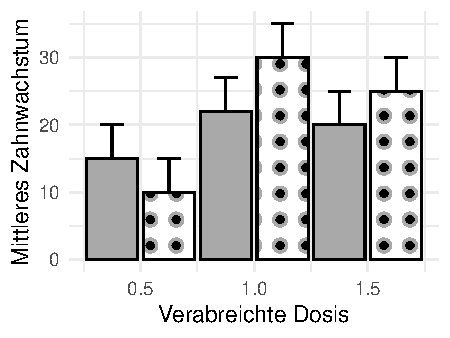
\includegraphics[width=\maxwidth]{img/mc-anova-02-a-1} 

}




Welche Aussage ist richtig im Bezug auf eine zweifaktorielle ANOVA?



\begin{enumerate}
\item [\textbf{A} \msquare] Eine starke Interaktion ist zu erwarten. Die Geraden schneiden sich und die Abst{"a}nde sind nicht gleichbleibend.
\item [\textbf{B} \msquare] Keine Interaktion liegt vor. Die Geraden scheiden sich und laufen nicht parallel.
\item [\textbf{C} \msquare] Eine leichte Interaktion ist zu erwarten. Die Geraen schneiden sich noch nicht, aber die Abst{"a}nde unterscheiden sich stark.
\item [\textbf{D} \msquare] Eine starke Interaktion liegt vor. Die Geraden laufen parallel und schneiden sich nicht.
\item [\textbf{E} \msquare] Keine Interaktion ist zu erwatzen. Die Geraden der Verabreichungsmethode laufen parallel und mit {"a}hnlichen Abst{"a}nden.
\end{enumerate} 

\section{Aufgabe \hfill (2 Punkte)}

Eine einfaktorielle ANOVA berechnet eine Teststatistik um zu die Nullhypothese abzulehnen. Welche Aussage {\"u}ber die Teststatistik der ANOVA ist richtig?



\begin{enumerate}
\item [\textbf{A} \msquare] Die ANOVA berechnet die T-Statistik indem den Mittelwertsunterschied der Gruppen simultan durch die Standardabweichung der Gruppen teilt. Wenn die T-Statistik h{"o}her als 1.96 ist, kann die Nullhypothese abgelehnt werden.
\item [\textbf{B} \msquare] Die ANOVA berechnet die F-Statistik indem die MS der Behandlung durch die MS des Fehlers geteilt werden. Wenn die F-Statistik sich der 0 ann{"a}hert kann die Nullhypothese nicht abgelehnt werden.
\item [\textbf{C} \msquare] Die ANOVA berechnet die F-Statistik indem die MS des Fehlers durch die MS der Behandlung geteilt werden. Wenn die F-Statistik sich der 1 ann{"a}hert kann die Nullhypothese nicht abgelehnt werden.
\item [\textbf{D} \msquare] Die ANOVA berechnet die T-Statistik aus der Multiplikation der MS Behandlung mit der MS der Fehler. Wenn die F-Statistik 0 ist, kann die Nullhypothese abgelehnt werden.
\item [\textbf{E} \msquare] Die ANOVA berechnt die F-Statistik aus den SS Behandlung geteilt durch die SS Fehler.
\end{enumerate} 

\section{Aufgabe \hfill (2 Punkte)}




Sie haben das abstrakte Modell $Y \sim X$ mit $X$ als Faktor mit zwei
Leveln vorliegen. Welche Aussage {\"u}ber $s^2_1 \neq s^2_2$ ist richtig?



\begin{enumerate}
\item [\textbf{A} \msquare] Es liegt Varianzhomogenit{"a}t vor.
\item [\textbf{B} \msquare] Es handelt sich um ein balanciertes Design.
\item [\textbf{C} \msquare] Es handelt sich um ein unbalanciertes Design
\item [\textbf{D} \msquare] Es handelt sich um abh{"a}ngige Beobachtungen.
\item [\textbf{E} \msquare] Es liegt Varianzhetrogenit{"a}t vor.
\end{enumerate} 

\section{Aufgabe \hfill (2 Punkte)}

Die Mindestanzahl an Beobachtungen f{\"u}r eine Zelle der Vierfeldertafel bei
der Nutzung eines Chi-Quadrat-Testes ist...



\begin{enumerate}
\item [\textbf{A} \msquare] 10 Beobachtungen
\item [\textbf{B} \msquare] 1 Beobachtung
\item [\textbf{C} \msquare] 5 Beobachtungen
\item [\textbf{D} \msquare] 2 Beobachtungen
\item [\textbf{E} \msquare] 0 Beobachtungen
\end{enumerate} 

\section{Aufgabe \hfill (2 Punkte)}




Berechnen Sie die Korrelation \textit{r} zwischen $x$ mit 7, 15, 8, 14 und 14 sowie $y$ mit 8, 4, 9, 17 und 7.  Nutzen Sie folgende Formel:

\begin{equation*}
  r_{x,y} = \cfrac{s_{x,y}}{s_x \cdot s_y}
\end{equation*}



\begin{enumerate}
\item [\textbf{A} \msquare] Es ergibt sich eine Korrelation von 0
\item [\textbf{B} \msquare] Es ergibt sich eine Korrelation von 1.03
\item [\textbf{C} \msquare] Es ergibt sich eine Korrelation von 0.03
\item [\textbf{D} \msquare] Es ergibt sich eine Korrelation von -0.03
\item [\textbf{E} \msquare] Es ergibt sich eine Korrelation von 0
\end{enumerate} 

\section{Aufgabe \hfill (2 Punkte)}




Berechnen Sie die Kovarianz $s_{x,y}$ und die Korrelation
\textit{r} zwischen $x$ mit 7, 13, 10, 0 und 13 sowie $y$ mit 14, 19, 14, 16 und 19.
\begin{equation*}
  r_{x,y} = \cfrac{s_{x,y}}{s_x \cdot s_y}
\end{equation*}



\begin{enumerate}
\item [\textbf{A} \msquare] Es ergibt sich eine Kovarianz von 300.76 sowie eine Korrelation von -0.49
\item [\textbf{B} \msquare] Es ergibt sich eine Kovarianz von -6.7 sowie eine Korrelation von 0.24
\item [\textbf{C} \msquare] Es ergibt sich eine Kovarianz von 6.7 sowie eine Korrelation von 0.49
\item [\textbf{D} \msquare] Es ergibt sich eine Kovarianz von 6.7 sowie eine Korrelation von -0.49
\item [\textbf{E} \msquare] Es ergibt sich eine Kovarianz von 44.89 sowie eine Korrelation von 0.24
\end{enumerate} 

\section{Aufgabe \hfill (2 Punkte)}




Berechnen Sie den Mittelwert und Standardabweichung von $y$ mit 15, 10, 11, 9 und 10.



\begin{enumerate}
\item [\textbf{A} \msquare] Es ergibt sich 12 +/- 1.175
\item [\textbf{B} \msquare] Es ergibt sich 10 +/- 2.75
\item [\textbf{C} \msquare] Es ergibt sich 11 +/- 5.5
\item [\textbf{D} \msquare] Es ergibt sich 11 +/- 1.175
\item [\textbf{E} \msquare] Es ergibt sich 11 +/- 2.35
\end{enumerate}

\section{Aufgabe \hfill (2 Punkte)}




Berechnen Sie den Median und das IQR von $x$ mit 12, 20, 19, 29, 27, 28 und 51.



\begin{enumerate}
\item [\textbf{A} \msquare] Es ergibt sich 27 +/- 29
\item [\textbf{B} \msquare] Es ergibt sich 27 +/- 19
\item [\textbf{C} \msquare] Es ergibt sich 27 [19, 29]
\item [\textbf{D} \msquare] Es ergibt sich 27 [19, 29]
\item [\textbf{E} \msquare] Es ergibt sich 27 +/- 19
\end{enumerate} 

\section{Aufgabe \hfill (2 Punkte)}

Eine der g{\"a}ngigsten Methode der Statistik um einen Fehler zu bestimmen ist...



\begin{enumerate}
\item [\textbf{A} \msquare] ... die Methode des absoluten Abstands.
\item [\textbf{B} \msquare] ... die Methode des absoluten, quadrierten Abstands.
\item [\textbf{C} \msquare] ... die Methode der aufaddierten, absoluten Abst{"a}nde.
\item [\textbf{D} \msquare] ... die kleinste Quadrate Methode oder auch least square method genannt.
\item [\textbf{E} \msquare] ... das Produkt der kleinsten Quadrate.
\end{enumerate} 

\section{Aufgabe \hfill (2 Punkte)}

Welche Aussage {\"u}ber \textit{ordinary mean} und \textit{marginal mean} ist richtig? 



\begin{enumerate}
\item [\textbf{A} \msquare] Der Begriff \textit{ordinary mean} beschreibt die einzelnen Mittelwerte der Level eines Faktors wohingegen der \textit{marginal mean} den Mittelwert {"u}ber alle Level des Faktors wiedergibt.
\item [\textbf{B} \msquare] Der Begriff \textit{ordinary mean} beschreibt einen unbedeutenden Mittelwert und \textit{marginal mean} einen Randmittelwert.
\item [\textbf{C} \msquare] Der Begriff \textit{ordinary mean} beschreibt die Mittelwerte eines Faktors wohingegen der \textit{marginal mean} die einzelnen Level betrachtet.
\item [\textbf{D} \msquare] Der Begriff \textit{ordinary mean} beschreibt einen einzelnen Mittelwert eines Levels eines Faktors wohingegen der \textit{marginal mean} die unbedeutenden Mittelwerte beschreibt.
\item [\textbf{E} \msquare] Der Begriff \textit{ordinary mean} beschreibt gew{"o}hnliche Mittelwerte und wohingegen \textit{marginal mean} kleine Mittelwerte beschreibt.
\end{enumerate} 

\section{Aufgabe \hfill (2 Punkte)}



Die empfohlene Mindestanzahl an Beobachtungen f{\"u}r einen Dotplot sind...



\begin{enumerate}
\item [\textbf{A} \msquare] 2-5 Beobachtungen.
\item [\textbf{B} \msquare] 1 Beobachtung.
\item [\textbf{C} \msquare] 5 und mehr Beobachtungen.
\item [\textbf{D} \msquare] mindestens 20 Beobachtungen.
\item [\textbf{E} \msquare] 10 Beobachtungen.
\end{enumerate} 

\section{Aufgabe \hfill (2 Punkte)}



Mit einem Boxplot wird Folgendes in der Statistik und der explorativen Datenanalyse haupts{\"a}chlich dargestellt.



\begin{enumerate}
\item [\textbf{A} \msquare] Die Eigenschaften von Daten aufgeteilt nach zwei Gruppen eines Faktors $x$.
\item [\textbf{B} \msquare] Die Verteilung von Daten. Meistens dem Outcome oder auch $y$ genannt. Hierbei ist eine hohe Fallzahl notwendig mit mehr als 20 Beoabchtungen.
\item [\textbf{C} \msquare] Die Verteilung von Daten. Meistens dem Outcome oder auch $y$ genannt. Die Darstellung ist auch mit einer kleinen Fallzahl von Minimum 5 Beoabchtungen m{"o}glich.
\item [\textbf{D} \msquare] Die Verteilung von Daten. Auch 2 bis 5 Beonachtungen k{"o}nnen noch dargestellt werden.
\item [\textbf{E} \msquare] Die Eigenschaften von Daten anhand der fehlenden Werte und den Leveln eines Faktors $x$.
\end{enumerate}

\section{Aufgabe \hfill (2 Punkte)}

Price et al. (2016) untersuchte die Auswirkungen des Bergbaus und der
Talauff{\"u}llung auf den Bestand und die H{\"a}ufigkeit von Bachsalamandern. Um
den Effekt zu Berechnen nutze Price et al. (2016) eine Possion-Regression
auf die Anzahl an aufgefundenen Bachsalamandern an den jeweiligen
Suchorten. Welche Aussage zur Possion-Regression auf Z{\"a}hldaten ist richtig?






\begin{enumerate}
\item [\textbf{A} \msquare] Die Possion-Regression sch{"a}tzt nur einen Verteilungsparameter. Deshalb muss {"u}berpr{"u}ft werden, ob Overdispersion vorliegt. Mit einer gesch{"a}tzen Overdispersion von 3.05 liegt Overdispersion vor. Damit kann keine Possion-Regression gerechnet werden. Die L{"o}sung ist eine Gaussian Regression mit Nullanpassung.
\item [\textbf{B} \msquare] Die Possion-Regression sch{"a}tzt zwei Verteilungsparameter. Deshalb muss {"u}berpr{"u}ft werden, ob Overdispersion vorliegt. Mit einer gesch{"a}tzen Overdispersion von 3.05 liegt keine Overdispersion vor.
\item [\textbf{C} \msquare] Die Possion-Regression sch{"a}tzt drei Verteilungsparameter. Deshalb muss {"u}berpr{"u}ft werden, ob Overdispersion vorliegt. Mit einer gesch{"a}tzen Overdispersion von 3.05 liegt Overdispersion vor. Die L{"o}sung ist die Nutzung von nur zwei der drei Verteilungsparameter: $\gamma_1$ und $\gamma_3$.
\item [\textbf{D} \msquare] Die Possion-Regression sch{"a}tzt nur einen Verteilungsparameter. Deshalb muss {"u}berpr{"u}ft werden, ob Overdispersion vorliegt. Mit einer gesch{"a}tzen Overdispersion von 3.05 liegt keine Overdispersion vor. Overdispersion liegt vor, wenn die gesch{"a}tzte Overdispersion unter 1 liegt.
\item [\textbf{E} \msquare] Die Possion-Regression sch{"a}tzt nur einen Verteilungsparameter. Deshalb muss {"u}berpr{"u}ft werden, ob Overdispersion vorliegt. Mit einer gesch{"a}tzen Overdispersion von 3.05 liegt Overdispersion vor. Die L{"o}sung ist die Nutzung einer anderen Verteilungsfamilie wie die Quasipossion Verteilung.
\end{enumerate}

\section{Aufgabe \hfill (2 Punkte)}

In dem folgenden Histogramm von $n = 200$ Pflanzen ist welche Verteilung
mit welchen korrekten Verteilungsparametern dargestellt?



{\centering 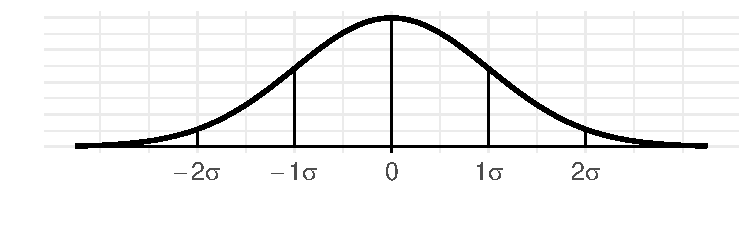
\includegraphics[width=\maxwidth]{img/mc-distribution-02-a-1} 

}







\begin{enumerate}
\item [\textbf{A} \msquare] Eine rechtsschiefe, multivariate Normalverteilung.
\item [\textbf{B} \msquare] Eine Standardnormalverteilung mit N(0,1).
\item [\textbf{C} \msquare] Es handelt sich um eine Poisson-Verteilung mit Pois(15).
\item [\textbf{D} \msquare] Es handelt sich um eine Normalverteilung mit N(15, 5).
\item [\textbf{E} \msquare] Es handelt sich um eine Binomial-Verteilung mit Binom(10).
\end{enumerate}

\section{Aufgabe \hfill (2 Punkte)}




Price et al. (2016) untersuchte die Auswirkungen des Bergbaus und der
Talauff{\"u}llung auf den Bestand und die H{\"a}ufigkeit von Bachsalamandern. Um
den Effekt zu Berechnen nutze Price et al. (2016) eine Possion-Regression
auf die Anzahl an aufgefundenen Bachsalamandern an den jeweiligen
Suchorten. Nach einer statistischen Beratung wurde Ihm nahegelegt auf
Overdispersion zu achten, wenn er statistische Aussagen zur Signifikanz
treffen will. Price et al. (2016) sch{\"a}tzt zwei Modelle. Modell 1 mit einer
Possion Verteilung und Modell 2 mit einer Quasi-Poisson Verteilung. Welche
Aussage zu einer gesch{\"a}tzen Overdispersion von 3.02 ist
richtig?




\begin{enumerate}
\item [\textbf{A} \msquare] Bei einer gesch{"a}tzen Overdispersion h{"o}her als 1.5 ist von keiner Overdispersion in den Daten auszugehen. Dennoch sind die p-Werte zu klein, dass diese p-Werte nat{"u}rlich entstanden sein k{"o}nnten. Die p-Werte m{"u}ssen adjustiert werden.
\item [\textbf{B} \msquare] Bei einer gesch{"a}tzen Overdispersion h{"o}her als 1.5 ist von Overdispersion in den Daten auszugehen. Daher wird die Varianz systematisch untersch{"a}tzt, was zu h{"o}heren p-Werten f{"u}hrt. Daher gibt es weniger signifikante Ergebnisse als es in Wirklichkeit gibt. Daher ist das Modell 1 die bessere Wahl.
\item [\textbf{C} \msquare] Bei einer gesch{"a}tzen Overdispersion h{"o}her als 1.5 ist von Overdispersion in den Daten auszugehen. Daher wird die Varianz systematisch untersch{"a}tzt, was zu kleineren p-Werten f{"u}hrt. Daher gibt es mehr signifikante Ergebnisse als es in Wirklichkeit gibt. Daher ist das Modell 2 die bessere Wahl.
\item [\textbf{D} \msquare] Bei einer gesch{"a}tzen Overdispersion h{"o}her als 1.5 ist von Overdispersion in den Daten auszugehen. Daher wird die Varianz systematisch {"u}bersch{"a}tzt, was zu h{"o}heren p-Werten f{"u}hrt. Daher gibt es mehr signifikante Ergebnisse als es in Wirklichkeit gibt. Daher ist das Modell 1 die bessere Wahl
\item [\textbf{E} \msquare] Das vergleichen von verschiedenen Modellen muss erst {"u}ber ein AIC Kriterium erfolgen. Die Absch{"a}tzung {"u}ber die Overdispersion ist nicht notwendig. Die Varianzen werden sp{"a}ter in einer ANOVA adjustiert. Die Confounder Adjustierung.
\end{enumerate}

\section{Aufgabe \hfill (2 Punkte)}

In einem Zuchtexperiment messen wir die Ferkel verschiedener Sauen. Die
Ferkel einer Muttersau sind daher im statistischen Sinne... 



\begin{enumerate}
\item [\textbf{A} \msquare] Untereinander unabh{"a}ngig. Sollten die M{"u}tter verwandt sein, so ist die Varianzstruktur {"a}hnlich und muss modelliert werden.
\item [\textbf{B} \msquare] Untereinander unabh{"a}ngig. Die Ferkel sind eigenst{"a}ndig und ben{"o}tigen keine zus{"a}tzliche Behandlung.
\item [\textbf{C} \msquare] Untereinander stark korreliert. Die Ferkel sind von einer Mutter und sommit miteinander korreliert. Dies wird in der Statistik jedoch meist nicht modelliert.
\item [\textbf{D} \msquare] Untereinander abh{"a}ngig. Die Ferkel stammen von einem Muttertier und haben vermutliche eine {"a}hnliche Varianzstruktur.
\item [\textbf{E} \msquare] Untereinander abh{"a}ngig, wenn die M{"u}tter ebenfalls miteinander verwandt sind. Erst die Abh{"a}ngigkeit 2. Grades wird in der Statistik modelliert.
\end{enumerate}

\section{Aufgabe \hfill (2 Punkte)}




Sie haben das abstrakte Modell $y \sim x_1 + x_2$ vorliegen. Welche Aussage {\"u}ber
X ist richtig?



\begin{enumerate}
\item [\textbf{A} \msquare] X beinhaltet mehrere Spalten. Die Spalten geben die Verteilungsfamilie vor.
\item [\textbf{B} \msquare] X beinhaltet mehrere Spalten. Die Spalten enthalten die Behandlung und weitere potenzielle Einflussvariablen
\item [\textbf{C} \msquare] X beinhaltet die Zeilen. Die Zeilen geben die Verteilungsfamilie vor.
\item [\textbf{D} \msquare] X beinhaltet eine Spalte. Die Spalte gibt nicht die Verteilungsfamilie vor.
\item [\textbf{E} \msquare] X beinhaltet eine Spalte. Die Spalte gibt die Verteilungsfamilie vor.
\end{enumerate}

\section{Aufgabe \hfill (2 Punkte)}




Sie haben das Modell $Y \sim X$ vorliegen und wollen nun ein
pr{"a}diktives Modell rechnen. Welche Aussage ist richtig?



\begin{enumerate}
\item [\textbf{A} \msquare] Ein pr{"a}diktives Modell m{"o}chte die Zusammenh{"a}nge von X auf Y modellieren. Hierbei geht es um die Effekte von X auf Y. Man sagt, wenn X um 1 ansteigt {"a}ndert sich Y um einen Betrag $\beta$.
\item [\textbf{B} \msquare] Ein pr{"a}diktives Modell ben{"o}tigt mindestens eine Fallzahl von {"u}ber 100 Beobachtungen und darf keine fehlenden Werte beinhalten. Die Varianzkomponenten m{"u}ssen homogen sein.
\item [\textbf{C} \msquare] Ein pr{"a}diktives Modell wird auf einem Trainingsdatensatz trainiert und anschliessend {"u}ber eine explorative Datenanalyse validiert. Signifikanzen {"u}ber $\beta_i$ k{"o}nnen hier nicht festgestellt werden.
\item [\textbf{D} \msquare] Ein pr{"a}diktives Modell basiert auf einem Traingsdatensatz und einem Testdatensatz. Auf dem Trainingsdatensatz wird das Modell trainiert und auf dem Testdatensatz validiert.
\item [\textbf{E} \msquare] Ein pr{"a}diktives Modell schliesst grunds{"a}tzlich lineare Modell aus. Es muss ein Graph gefunden werden, der alle Punkte beinhaltet. Erst dann kann das $R^2$ berechnet werden.
\end{enumerate}

\section{Aufgabe \hfill (2 Punkte)}



In der folgenden Abbildung ist der Zusammenhang vom Modell zu der linearen
Regression und der ANOVA skizziert.

\begin{center}
  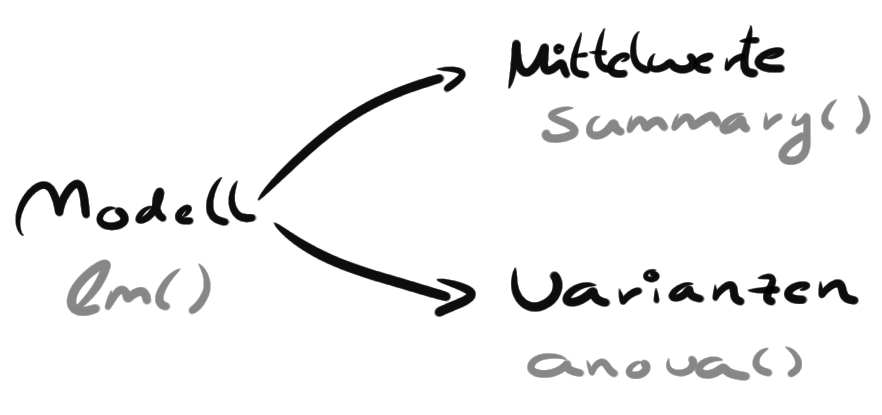
\includegraphics[width = 9cm]{/Users/kruppajo/Documents/GitHub/exam/question/img/mc-modeling-03}
\end{center}

Welche der folgenden Aussagen ist richtig?



\begin{enumerate}
\item [\textbf{A} \msquare] Die Effektsch{"a}tzer aus einem Modell, erlauben es nur einen Mittelwertsvergleich zu rechnen.
\item [\textbf{B} \msquare] Die Effektsch{"a}tzer aus einem Modell, in diesem Fall ein lineares Modell, erlauben es sowohl eine ANOVA zurechnen sowie auch eine Zusammenfassung der Mittelwerte zu betrachten.
\item [\textbf{C} \msquare] Die Effektsch{"a}tzer aus einem Modell, erlauben es nur eine ANOVA zu rechnen. 
\item [\textbf{D} \msquare] Die Effektsch{"a}tzer aus einem Modell, in diesem Fall ein lineares Modell, erlauben es nur eine ANOVA zurechnen oder eine Zusammenfassung der Mittelwerte zu betrachten. Beides ist nicht m{"o}glich.
\item [\textbf{E} \msquare] Die Effektsch{"a}tzer aus einem Modell, in diesem Fall ein polynomes Modell, erlauben es sowohl eine ANOVA zurechnen sowie auch eine Zusammenfassung der Mittelwerte zu betrachten.
\end{enumerate}

\section{Aufgabe \hfill (2 Punkte)}

In der Statistik werden die Daten D modelliert in dem ein Modell der Form
$Y \sim X$ aufgestellt wird. Welche statistische Kenngr{\"o}sse wird modelliert? 



\begin{enumerate}
\item [\textbf{A} \msquare] Die Varianzstruktur wird modelliert.
\item [\textbf{B} \msquare] Die Mittelwerte werden modelliert.
\item [\textbf{C} \msquare] Die Varianz der X unabh{"a}ngig vom Y wird modelliert.
\item [\textbf{D} \msquare] Die X werden modelliert.
\item [\textbf{E} \msquare] Die Y werden modelliert.
\end{enumerate}

\section{Aufgabe \hfill (2 Punkte)}



Sie f{\"u}hren ein Experiment zur Behandlung von Klaueninfektionen bei K{\"u}hen
durch. Bei 4 Tieren finden Sie eine Erkrankung der Klauen vor und
12 Tiere sind gesund. Welche Aussage {\"u}ber den Risk ratio
Effektsch{\"a}tzer ist richtig?



\begin{enumerate}
\item [\textbf{A} \msquare] Es ergibt sich ein Risk ratio von 0.25, da es sich um ein Anteil handelt.
\item [\textbf{B} \msquare] Es ergibt sich ein Risk ratio von 0.33, da es sich um eine Chancenverh{"a}ltnis handelt.
\item [\textbf{C} \msquare] Es ergibt sich ein Risk ratio von 3, da es sich um ein Anteil handelt.
\item [\textbf{D} \msquare] Es ergibt sich ein Risk ratio von 0.33, da es sich um ein Anteil handelt.
\item [\textbf{E} \msquare] Es ergibt sich ein Risk ratio von 0.25, da es sich um eine Chancenverh{"a}ltnis handelt.
\end{enumerate}

\section{Aufgabe \hfill (2 Punkte)}




Welche Aussage {\"u}ber die nicht-parametrische Statistik ist richtig?



\begin{enumerate}
\item [\textbf{A} \msquare] Die nicht-parametrische Statistik basiert auf dem Sch{"a}tzen von Parametern aus einer festgelegten Verteilung. Daher gibt es auch direkt zu interpretierenden Effektsch{"a}tzer.
\item [\textbf{B} \msquare] Die nicht-parametrische Statistik ist ein Vorg{"a}nger der parametrischen Statistik und wurde wegen dem Mangel an Effektsch{"a}tzern nicht mehr ab 1960 genutzt.
\item [\textbf{C} \msquare] Die nicht-parametrische Statistik basiert auf R{"a}ngen. Daher gibt es auch direkt zu interpretierenden Effektsch{"a}tzer.
\item [\textbf{D} \msquare] Die nicht-parametrische Statistik basiert auf dem Sch{"a}tzen von Parametern aus einer a priori festgelegten Verteilung. Daher gibt es auch direkt zu interpretierenden Effektsch{"a}tzer.
\item [\textbf{E} \msquare] Die nicht-parametrische Statistik basiert auf R{"a}ngen. Daher wird jeder Zahl ein Rang zugeteilt. Nur auf den R{"a}ngen wird die Auswertung gerechnet. Daher gibt es auch keinen direkt zu interpretierenden Effektsch{"a}tzer.
\end{enumerate}

\section{Aufgabe \hfill (2 Punkte)}

Die Randomisierung von Beobachtungen bzw. Samples zu den Versuchseinheiten
ist bedeutend in der Versuchsplanung. Welche der folgenden Aussagen ist richtig?



\begin{enumerate}
\item [\textbf{A} \msquare] Randomisierung sorgt f{"u}r Strukturgleichheit und erlaubt erst von der Stichprobe auf die Grundgesamtheit zur{"u}ckzuschliessen.
\item [\textbf{B} \msquare] Randomisierung war bis 1952 bedeutend, wurde dann aber in Folge besserer Rechnerleistung nicht mehr verwendet. Aktuelle Statistik nutzt keine Randomisierung mehr.
\item [\textbf{C} \msquare] Randomisierung bringt starke Unstrukturiertheit in das Experiment und erlaubt erst von der Stichprobe auf die Grundgesamtheit zur{"u}ckzuschliessen.
\item [\textbf{D} \msquare] Randomisierung erlaubt erst die Mittelwerte zu sch{"a}tzen. Ohne Randomisierung keine Mittelwerte.
\item [\textbf{E} \msquare] Randomisierung erlaubt erst die Varianzen zu sch{"a}tzen. Ohne eine Randomisierung ist die Berechnung von Mittelwerten und Varianzen nicht m{"o}glich.
\end{enumerate}

\section{Aufgabe \hfill (2 Punkte)}

Wenn Sie einen Datensatz erstellen, dann ist es ratsam die Spalten und die
Eintr{\"a}ge in englischer Sprache zu verfassen, wenn Sie sp{\"a}ter die Daten in
\Rlogo auswerten wollen. Welcher folgende Grund ist richtig?



\begin{enumerate}
\item [\textbf{A} \msquare] Es gibt keinen Grund nicht auch deutsche W{"o}rter zu verwenden. Es ist ein Stilmittel.
\item [\textbf{B} \msquare] Programmiersprachen k{"o}nnen nur englische Begriffe verarbeiten. Zus{"a}tzliche Pakete k{"o}nnen zwar geladen werden, aber meist funktionieren diese Pakete nicht richtig. Deutsch ist International nicht bedeutend genug.
\item [\textbf{C} \msquare] Alle Funktionen und auch Anwendungen sind in \Rlogo in englischer Sprache. Die Nutzung von deutschen W{"o}rtern ist nicht schick und das ist zu vermeiden.
\item [\textbf{D} \msquare] Im Allgemeinen haben Programmiersprachen Probleme mit Umlauten und Sonderzeichen, die in der deutschen Sprache vorkommen. Eine Nutzung der englischen Sprache umgeht dieses Problem auf einfache Art.
\item [\textbf{E} \msquare] Die Spracherkennung von \Rlogo ist nicht in der Lage Deutsch zu verstehen.
\end{enumerate}

\section{Aufgabe \hfill (2 Punkte)}

Bei der explorativen Datenanalyse (EDA) in \Rlogo gibt es eine richtige Abfolge von Prozessschritten, auch \textit{Circle of life} genannt. Wie lautet die richtige Reihenfolge f{\"u}r die Erstellung einer EDA?



\begin{enumerate}
\item [\textbf{A} \msquare] Wir lesen die Daten ein und mutieren die Daten. Dabei ist wichtig, dass wir nicht das Paket \texttt{tidyverse} nutzen, da dieses Paket veraltet ist. {"U}ber die Funktion \texttt{library(tidyverse)} entfernen wir das Paket von der Analyse.
\item [\textbf{B} \msquare] Wir transformieren die Spalten {"u}ber \texttt{mutate()} in ein \texttt{tibble} und k{"o}nnen dann {"u}ber \text{ggplot()} uns die Abbildungen erstellen lassen. Dabei beachten wir das wir keine Faktoren in den Daten haben.
\item [\textbf{C} \msquare] Wir lesen als erstes die Daten {"u}ber \texttt{read\_excel()} ein, transformieren die Spalten {"u}ber \texttt{mutate()} in die richtige Form und k{"o}nnen dann {"u}ber \text{ggplot()} uns die Abbildungen erstellen lassen.
\item [\textbf{D} \msquare] Wir lesen als erstes die Daten {"u}ber \texttt{read\_excel()} ein, transformieren die Spalten {"u}ber \texttt{mutate()} in die richtige Form und k{"o}nnen dann  {"u}ber \text{ggplot()} uns die Abbildungen erstellen lassen. Wichtig ist, dass wir keine Faktoren sondern nur numerische Variablen vorliegen haben.
\item [\textbf{E} \msquare] Wir lesen die Daten {"u}ber eine generische Funktion \texttt{read()} ein und m{"u}ssen dann die Funktion \texttt{ggplot()} nur noch installieren. Dann haben wir die Abbildungen als \texttt{*.png} vorliegen.
\end{enumerate}

\section{Aufgabe \hfill (2 Punkte)}



In einem Stallexperiment mit $n = 104$ Ferkeln wurden verschiedene
Outcomes gemessen: der Gewichtszuwachs, {\"U}berleben nach 21 Tagen sowie
Anzahl Verletzungen pro 7 Tagen. Zwei Lichtregime wurden als
Einflussfaktor gemessen. Sie erhalten den \Rlogo Output der Funktion
\texttt{tidy()} einer simplen $possion$ linearen
Regression. Welche Aussage {\"u}ber den \textbf{Effekt} ist richtig?

\begin{table}[!h]
\centering
\begin{tabular}{ccc}
\toprule
term & estimate & std.error\\
\midrule
(Intercept) & 0.88 & 0.08\\
light\_binhigh & -0.15 & 0.14\\
\bottomrule
\end{tabular}
\end{table}





\begin{enumerate}
\item [\textbf{A} \msquare] In einer possion Regression wird die Mittelwertsdifferenz betrachtet. Daher ist der Effekt zwischen den beiden Lichtregimen eine Gewichts{"a}nderung von -0.15
\item [\textbf{B} \msquare] In einer possion Regression muss f{"u}r die Interpretation des Effektes das $\beta_1$ quadriert werden. Somit liegt das OR bei 0.02
\item [\textbf{C} \msquare] In einer possion Regression berechnet man das RR. Daher muss der Sch{"a}tzer des Effektes $\beta_1$ noch quadriert werden. Somit liegt das RR bei 0.02
\item [\textbf{D} \msquare] Eine possion Regression basiert auf dem maximum Likelihood Prinzip. Hierbei kann kein Effekt beschrieben werden. Im Zweifel hilft aber eine Quadrierung der Fehlerqudrate $\epsilon$.
\item [\textbf{E} \msquare] In einer possion Regression kann kein Effekt roh interpretiert werden. Es muss erst eine Confounderadjustierung durchgef{"u}hrt werden.
\end{enumerate}

\section{Aufgabe \hfill (2 Punkte)}

In einer linearen Regression werden die $\epsilon$ oder Residuen
gesch{\"a}tzt. Welcher Verteilung folgen die Residuen bei einer optimalen
Modellierung? 



\begin{enumerate}
\item [\textbf{A} \msquare] Die Residuen sind binomialverteilt.
\item [\textbf{B} \msquare] Die Residuen folgen einer Poissonverteilung mit Pois(0).
\item [\textbf{C} \msquare] Die Residuen sind normalverteilt mit $\mathcal{N}(\bar{y}, s^2)$.
\item [\textbf{D} \msquare] Die Residuen sind normalverteilt mit $\mathcal{N}(0, s^2)$.
\item [\textbf{E} \msquare] Die Residuen sind normalverteilt mit $\mathcal{N}(0, 1)$.
\end{enumerate}

\section{Aufgabe \hfill (2 Punkte)}

Welche Aussage {\"u}ber das \textit{generalisierte lineare Modell (GLM)} ist richtig?  



\begin{enumerate}
\item [\textbf{A} \msquare] Das GLM erlaubt auch nicht normalverteilte Residuen in der Sch{"a}tzung der Regressionsgrade.
\item [\textbf{B} \msquare] Das GLM ist ein faktisch maschineller Lernalgorithmus, der selstst{"a}ndig die Verteilungsfamilie f{"u}r Y w{"a}hlt.
\item [\textbf{C} \msquare] Das GLM ist eine allgemeine Erweiterung der linearen Regression auf die Normalverteilung.
\item [\textbf{D} \msquare] Das GLM ist eine Vereinfachung des LM in R. Mit dem GLM lassen polygonale Regressionen rechnen.
\item [\textbf{E} \msquare] Das GLM erlaubt auch weitere Verteilungsfamilien f{"u}r das Y bzw. das Outcome in einer linearen Regression zu w{"a}hlen.
\end{enumerate}

\section{Aufgabe \hfill (2 Punkte)}



Sie rechnen in einer linearen Regression das Modell A und das Modell B. Nun
stellt sich die Frage, welches der beiden Modelle das bessere Modell
ist. Um die Modelle bewerten zu k{\"o}nnen berechnen Sie daf{\"u}r das AIC$_A$ f{\"u}r
Modell A mit 653 und f{\"u}r das Modell B das AIC$_B$ von
287. Welche Aussage {\"u}ber die beiden Modelle ist richtig?



\begin{enumerate}
\item [\textbf{A} \msquare] Da AIC$_A$ > AIC$_B$ ist das Modell A das bessere Modell.
\item [\textbf{B} \msquare] Da AIC$_A$ > 0 ist das Modell A das bessere Modell. Der AIC Wert f{"u}r B wird verworfen.
\item [\textbf{C} \msquare] Da AIC$_A$ < AIC$_B$ ist das Modell A das bessere Modell.
\item [\textbf{D} \msquare] Da AIC$_A$ < AIC$_B$ ist das Modell B das bessere Modell.
\item [\textbf{E} \msquare] Da AIC$_A$ > AIC$_B$ ist das Modell B das bessere Modell.
\end{enumerate}

\section{Aufgabe \hfill (2 Punkte)}

Sie rechnen in eine linearen Regression und erhalten folgenden QQ
Plot. Welche Aussage ist richtig?




{\centering 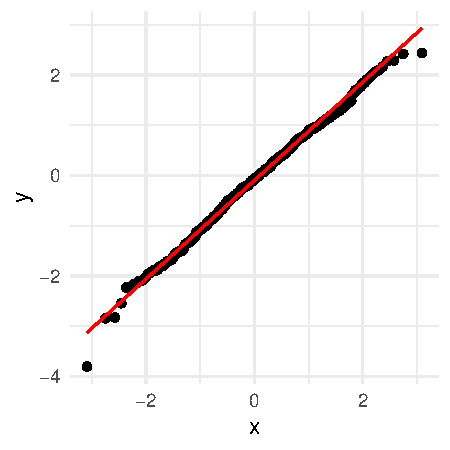
\includegraphics[width=\maxwidth]{img/mc-regression-05-a-1} 

}







\begin{enumerate}
\item [\textbf{A} \msquare] Die Annahme der normalverteilten Residuen ist erf{"u}llt. Die Punkte liegen zum {"u}berwiegenden Teil nicht auf der Geraden und Korrelation ist negativ.
\item [\textbf{B} \msquare] Die Annahme der normalverteilten Residuen ist nicht erf{"u}llt. Die Punkte liegen zum {"u}berwiegenden Teil nicht auf der Geraden.
\item [\textbf{C} \msquare] Die Annahme der normalverteilten Residuen ist nicht erf{"u}llt. Die Punkte liegen zum {"u}berwiegenden Teil auf der Geraden.
\item [\textbf{D} \msquare] Die Annahme der normalverteilten Residuen ist erf{"u}llt. Die Punkte liegen zum {"u}berwiegenden Teil auf der Geraden.
\item [\textbf{E} \msquare] Die Annahme der normalverteilten Residuen ist erf{"u}llt. Die Punkte liegen zum {"u}berwiegenden Teil nicht auf der Geraden.
\end{enumerate}

\section{Aufgabe \hfill (2 Punkte)}

Sie rechnen eine linearen Regression und erhalten folgenden Residual
Plot. Welche Aussage ist richtig?




{\centering 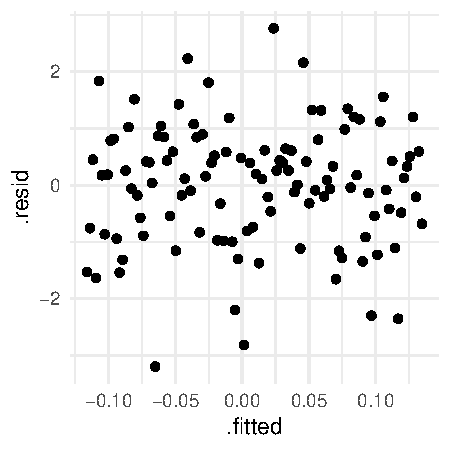
\includegraphics[width=\maxwidth]{img/mc-regression-06-a-1} 

}







\begin{enumerate}
\item [\textbf{A} \msquare] Die Annahme der normalverteilten Residuen ist nicht erf{"u}llt. Es ist kein Muster zu erkennen.
\item [\textbf{B} \msquare] Die Annahme der normalverteilten Residuen ist erf{"u}llt. Kein Muster ist zu erkennen und keine Outlier zu beobachten.
\item [\textbf{C} \msquare] Die Annahme der normalverteilten Residuen ist erf{"u}llt. Die Punkte liegen zum {"u}berwiegenden Teil auf der Diagonalen.
\item [\textbf{D} \msquare] Die Annahme der normalverteilten Residuen ist nicht erf{"u}llt. Vereinzelte Punkte liegen oberhalb bzw. unterhalb der Geraden um die 0 Linie weiter entfernt. Ein klares Muster ist zu erkennen.
\item [\textbf{E} \msquare] Die Annahme der normalverteilten Residuen ist erf{"u}llt. Es ist ein Muster zu erkennen.
\end{enumerate}

\section{Aufgabe \hfill (2 Punkte)}




Sie wollen ein Feldexperiment mit zwei D{\"u}ngestufen durchf{\"u}hren. Berechnen
Sie die ben{\"o}tigte Fallzahl mit $t_{1-\alpha/2} = 1.645$ und
$t_{1-\beta} = 1.282$ sowie $s = 2$ und
$\delta_0 = 1$. Es ergibt sich somit folgende Fallzahl.



\begin{enumerate}
\item [\textbf{A} \msquare] Es ergibt sich eine Fallzahl von 35
\item [\textbf{B} \msquare] Es ergibt sich eine Fallzahl von 138
\item [\textbf{C} \msquare] Es ergibt sich eine Fallzahl von 136
\item [\textbf{D} \msquare] Es ergibt sich eine Fallzahl von 69
\item [\textbf{E} \msquare] Es ergibt sich eine Fallzahl von 68
\end{enumerate}

\section{Aufgabe \hfill (2 Punkte)}

Welche Aussage zum mathematische Ausdruck $Pr(D|H_0)$ ist richtig? 



\begin{enumerate}
\item [\textbf{A} \msquare] Die Wahrscheinlichkeit f{"u}r die Nullhypothese, wenn die Daten wahr sind.
\item [\textbf{B} \msquare] Die Inverse der Wahrscheinlichkeit unter der die Nullhypothese nicht mehr die Alternativehypothese {"u}berdeckt.
\item [\textbf{C} \msquare] $Pr(D|H_0)$ ist die Wahrscheinlichkeit der Alternativehypothese und somit $1 - Pr(H_A)$
\item [\textbf{D} \msquare] $Pr(D|H_0)$ ist die Wahrscheinlichkeit die Daten D zu beobachten wenn die Nullhypothese wahr ist.
\item [\textbf{E} \msquare] Die Wahrscheinlichkeit der Daten unter der Nullhypothese in der Grundgesamtheit.
\end{enumerate}

\section{Aufgabe \hfill (2 Punkte)}

Das Falsifikationsprinzip besagt... 



\begin{enumerate}
\item [\textbf{A} \msquare] ... dass in der Wissenschaft immer etwas falsch sein muss. Sonst gebe es keinen Fortschritt.
\item [\textbf{B} \msquare] ... dass Modelle meist falsch sind und selten richtig.
\item [\textbf{C} \msquare] ... dass Fehlerterme in statistischen Modellen nicht verifiziert werden k{"o}nnen.
\item [\textbf{D} \msquare] ... dass Annahmen an statistische Modelle meist falsch sind.
\item [\textbf{E} \msquare] ... dass ein schlechtes Modell durch ein weniger schlechtes Modell ersetzt wird. Die Wissenschaft lehnt ab und verifiziert nicht.
\end{enumerate}

\section{Aufgabe \hfill (2 Punkte)}

Der Fehler 1. Art oder auch Signifikanzniveau $\alpha$ genannt, liegt bei
5\%. Welcher der folgenden Gr{\"u}nde f{\"u}r diese Festlegeung auf 5\% ist richtig?



\begin{enumerate}
\item [\textbf{A} \msquare] Im Rahmen eines langen Disputs zwischen Neyman und Fischer wurde $\alpha = 5\%$ festgelegt. Leider werden die Randbedingungen und Voraussetzungen an statistsiche Modelle heute immer wieder ignoriert.
\item [\textbf{B} \msquare] Der Begr{"u}nder der modernen Statistik, R. Fischer, hat die Grenze simuliert und berechnet. Dadurch ergibt sich dieser optimale Cut-Off.
\item [\textbf{C} \msquare] Der Wert ergab sich aus einer Auswertung von 1042 wissenschaftlichen Ver{"o}ffentlichungen zwischen 1914 und 1948. Der Wert $5\%$ wurde in $28\%$ der Ver{"o}ffentlichungen genutzt. Daher legte man sich auf diese Zahl fest.
\item [\textbf{D} \msquare] Auf einer Statistikkonferenz in Genf im Jahre 1942 wurde dieser Cut-Off nach langen Diskussionen festgelegt. Bis heute ist der Cut Off aber umstritten, da wegen dem 2. Weltkrieg viele Wissenschaftler nicht teilnehmen konnten.
\item [\textbf{E} \msquare] Die Festlegung von $\alpha = 5\%$ ist eine Kulturkonstante. Wissenschaftler ben{"o}tigt eine Schwelle f{"u}r eine statistische Testentscheidung, der Wert von $\alpha$ wurde aber historisch mehr zuf{"a}llig gew{"a}hlt.
\end{enumerate}

\section{Aufgabe \hfill (2 Punkte)}

Welche Aussage {\"u}ber die Power ist richtig?



\begin{enumerate}
\item [\textbf{A} \msquare] Die Power $1-\beta$ wird auf 80\% gesetzt. Damit liegt die Wahrscheinlichkeit f{"u}r die $H_0$ bei 20\%.
\item [\textbf{B} \msquare] Die Power $1-\beta$ wird auf 80\% gesetzt. Alle statistischen Tests sind so konstruiert, dass die $H_A$ mit 80\% "bewiesen wird".
\item [\textbf{C} \msquare] Die Power ist nicht in der aktuellen Testthorie mehr vertreten. Wir rechnen nur noch mit dem Fehler 1. Art.
\item [\textbf{D} \msquare] Die Power beschreibt die Wahrscheinlichkeit die $H_A$ abzulehnen. Wir testen die Power jedoch nicht.
\item [\textbf{E} \msquare] Es gilt $\alpha + \beta = 1$ und somit liegt $\beta$ meist bei 95\%.
\end{enumerate}

\section{Aufgabe \hfill (2 Punkte)}

Beim statistischen Testen wird \texttt{signal} mit \texttt{noise} zur
Teststatistik T verrechnet. Welche der Formel berechnet korrekt die
Teststatistik T?



\begin{enumerate}
\item [\textbf{A} \msquare] Es gilt $T = \cfrac{noise}{signal}$
\item [\textbf{B} \msquare] Es gilt $T = \cfrac{signal}{noise}$
\item [\textbf{C} \msquare] Es gilt $T = (signal \cdot noise)^2$
\item [\textbf{D} \msquare] Es gilt $T = \cfrac{signal}{noise^2}$
\item [\textbf{E} \msquare] Es gilt $T = signal \cdot noise$
\end{enumerate}

%% ------------------------------------------------------------

\section{Aufgabe \hfill (2 Punkte)}



In der Theorie zur statistischen Testentscheidung kann "`$H_0$ beibehalten obwohl die $H_0$ falsch ist"'
in welche richtige Analogie gesetzt werden?



\begin{enumerate}
\item [\textbf{A} \msquare] In die Analogie eines Rauchmelders: \textit{Alarm with fire}.
\item [\textbf{B} \msquare] In die Analogie eines brennenden Hauses ohne Rauchmelder: \textit{House without noise}.
\item [\textbf{C} \msquare] In die Analogie eines Rauchmelders: \textit{Fire without alarm}, dem $\beta$-Fehler.
\item [\textbf{D} \msquare] In die Analogie eines Feuerwehrautos: \textit{Car without noise}.
\item [\textbf{E} \msquare] In die Analogie eines Rauchmelders: \textit{Alarm without fire}, dem $\alpha$-Fehler.
\end{enumerate}

\section{Aufgabe \hfill (2 Punkte)}



Sie rechnen eine simple Poisson Regression. Welche Aussage bestreffend der
Konfidenzintervalle ist f{\"u}r die Poisson Regression richtig?



\begin{enumerate}
\item [\textbf{A} \msquare] Wenn die 0 im Konfidenzinterval enthalten ist, kann die Nullhypothese nicht abgelehnt werden.
\item [\textbf{B} \msquare] Wenn die Relevanzschwelle mit enthalten ist, kann die Nullhypothese abgelehnt werden.
\item [\textbf{C} \msquare] Wenn die 0 im Konfidenzinterval enthalten ist, kann die Nullhypothese abgelehnt werden.
\item [\textbf{D} \msquare] Wenn die Konfidenzintervalle den p-Wert der Regression enthalten, kann die Nullhypothese abgelehnt werden.
\item [\textbf{E} \msquare] Wenn die 1 im Konfidenzinterval enthalten ist, kann die Nullhypothese nicht abgelehnt werden.
\end{enumerate}

\section{Aufgabe \hfill (2 Punkte)}

In der Bio Data Science wird h{\"a}ufig mit sehr gro{\ss}en Datens{\"a}tzen
gerechnet. Historisch ergibt sich nun ein Problem bei der Auswertung der
Daten und deren Bewertung hinsichtlich der Signifikanz. Welche Aussage ist richtig?



\begin{enumerate}
\item [\textbf{A} \msquare] Relevanz und Signifikanz haben nichts miteinander zu tun. Daher gibt es auch keinen Zusammenhang zwischen hoher Fahlzahl (n > 10000) und einem signifikanten Test. Ein Effekt ist immer relevant und somit signifikant.
\item [\textbf{B} \msquare] Aktuell werden zu grosse Datens{"a}tze f{"u}r die g{"a}nigige Statistik gemessen. Daher wendet man maschinelle Lernverfahren f{"u}r kausale Modelle an. Hier ist die Relevanz gleich Signifikanz.
\item [\textbf{C} \msquare] Big Data ist ein Problem der parametrischen Statistik. Parameter lassen sich nur auf kleinen Datens{"a}tzen berechnen, da es sich sonst nicht mehr um eine Stichprobe im engen Sinne der Statistik handelt.
\item [\textbf{D} \msquare] Aktuell werden immer gr{"o}ssere Datens{"a}tze erhoben. Eine erh{"o}hte Fallzahl f{"u}hrt automatisch auch zu mehr signifikanten Ergebnissen, selbst wenn die eigentlichen Effekte nicht relevant sind.
\item [\textbf{E} \msquare] Aktuell werden immer gr{"o}ssere Datens{"a}tze erhoben. Dadurch wird auch die Varianz immer h{"o}her was automatisch zu mehr signifikanten Ergebnissen f{"u}hrt.
\end{enumerate}

\section{Aufgabe \hfill (2 Punkte)}

Welche statistische Masszahl erlaubt es \textit{Relevanz} mit
\textit{Signifikanz} zuverbinden? Welche Aussage ist richtig?



\begin{enumerate}
\item [\textbf{A} \msquare] Das OR. Als Chancenverh{"a}ltnis gibt es das Verh{"a}ltnis von Relevanz und Signifikanz wieder.
\item [\textbf{B} \msquare] Der p-Wert. Durch den Vergleich mit $\alpha$ l{"a}sst sich {"u}ber die Signifikanz entscheiden und der $\beta$-Fehler erlaubt {"u}ber die Power eine Einsch{"a}tzung der Relevanz.
\item [\textbf{C} \msquare] Die Teststatistik. Durch den Vergleich von $T_c$ zu $T_k$ ist es m{"o}glich die $H_0$ abzulehnen. Die Relevanz ergibt sich aus der Fl{"a}che rechts vom dem $T_c$-Wert.
\item [\textbf{D} \msquare] Das Konfidenzintervall. Durch die Visualizierung des Konfidenzintervals kann eine Relevanzschwelle vom Anwender definiert werden. Zus{"a}tzlich erlaubt das Konfidenzinterval auch eine Entscheidung {"u}ber die Signifikanz.
\item [\textbf{E} \msquare] Das $\Delta$. Durch die Effektst{"a}rke haben wir einen Wert f{"u}r die Relevanz, die vom Anwender bewertet werden muss. Da $\Delta$ antiproportional zum p-Wert ist, bedeutet auch ein hohes $\Delta$ ein sehr kleinen p-Wert.
\end{enumerate}

\section{Aufgabe \hfill (2 Punkte)}



Welche Aussage über die frequentistischen Testtheorie ist richtig?



\begin{enumerate}
\item [\textbf{A} \msquare] Wir machen Aussagen über die individuelle Wahrscheinlichkeit eines Effektes!
\item [\textbf{B} \msquare] Wir machen keine Aussagen über Wahrscheinlichkeiten!
\item [\textbf{C} \msquare] Wir machen Aussagen über den Effekt!
\item [\textbf{D} \msquare] Wir machen Aussagen über Wahrscheinlichkeiten!
\item [\textbf{E} \msquare] Wir machen Aussagen über Individuen!
\end{enumerate}

\section{Aufgabe \hfill (2 Punkte)}

Welche Aussage über den $p$-Wert und dem Signifikanzniveau $\alpha$ gleich 5\% ist richtig?



\begin{enumerate}
\item [\textbf{A} \msquare] Wir vergleichen die Effekte des $p$-Wertes mit den Effekten der Signifiaknzschwelle unter der Annahme der Nullhypothese.
\item [\textbf{B} \msquare] Wir vergleichen mit dem $p$-Wert und dem Signifikanzniveau $\alpha$ Wahrscheinlichkeiten und damit die absoluten Werte auf einem Zahlenstrahl, wenn die $H_0$ gilt.
\item [\textbf{C} \msquare] Wir vergleichen mit dem $p$-Wert und dem Signifikanzniveau $\alpha$ absolute Werte auf einem Zahlenstrahl und damit den Unterschied der Teststatistiken, wenn die $H_0$ gilt.
\item [\textbf{D} \msquare] Wir machen eine Aussage über die indivduelle Wahrscheinlichkeit des Eintretens der Nullhypothese $H_0$.
\item [\textbf{E} \msquare] Wir vergleichen mit dem $p$-Wert und dem Signifikanzniveau $\alpha$ Wahrscheinlichkeiten und damit die Flächen unter der Kurve der Teststatistik, wenn die $H_0$ gilt.
\end{enumerate}

\section{Aufgabe \hfill (2 Punkte)}

Welche Aussage {\"u}ber den t-Test ist richtig?



\begin{enumerate}
\item [\textbf{A} \msquare] Der t-Test vergleicht die Mittelwerte von zwei Gruppen unter der strikten Annahme von Varianzhomogenit{"a}t. Sollte keine Varianzhomogenit{"a}t vorliegen, so gibt es keine M{"o}glichkeit den t-Test in einer Variante anzuwenden.
\item [\textbf{B} \msquare] Der t-Test vergleicht die Mittelwerte von zwei Gruppen.
\item [\textbf{C} \msquare] Der t-Test ist ein Vortest der ANOVA und basiert daher auf dem Vergleich von Streuungsparametern
\item [\textbf{D} \msquare] Der t-Test vergleicht die Varianzen von mindestens zwei oder mehr Gruppen
\item [\textbf{E} \msquare] Der t-Test testet generell zu einem erh{"o}hten $\alpha$-Niveau von 20\%.
\end{enumerate}    

\section{Aufgabe \hfill (2 Punkte)}

Welche Aussage {\"u}ber den Welch t-Test ist richtig?



\begin{enumerate}
\item [\textbf{A} \msquare] Der Welch t-Test ist ein Post-hoc Test der ANOVA und basiert daher auf dem Vergleich der Varianz.
\item [\textbf{B} \msquare] Der Welch t-Test vergleicht die Mittelwerte von zwei Gruppen unter der strikten Annahme von Varianzhomogenit{"a}t.
\item [\textbf{C} \msquare] Der Welch t-Test ist die veraltete Form des Student t-Test und wird somit nicht mehr verwendet.
\item [\textbf{D} \msquare] Der Welch t-Test vergleicht die Varianz von zwei Gruppen.
\item [\textbf{E} \msquare] Der Welch t-Test wird angewendet, wenn Varianzheterogenit{"a}t zwischen den beiden zu vergleichenden Gruppen vorliegt.
\end{enumerate}  

\section{Aufgabe \hfill (2 Punkte)}

Nach einem Experiment mit f{\"u}nf Weizensorten ergibt eine ANOVA ($p = 0.041$)
einen signifikanten Unterschied f{\"u}r den Ertrag. Sie f{\"u}hren anschlie{\ss}end die
paarweisen t-Tests f{\"u}r alle Vergleiche der verschiedenen Weizensorten
durch. Nach der Adjustierung f{\"u}r multiples Testen ist kein p-Wert unter der
$\alpha$-Schwelle. Sie schauen sich auch die rohen, unadjustierten p-Werte
an und finden hier als niedrigsten p-Wert $p_{3-2} = 0.053$. Welche Aussage
ist richtig? 



\begin{enumerate}
\item [\textbf{A} \msquare] Die ANOVA testet auf der gesamten Fallzahl. Die einzelnen t-Tests immer nur auf einer kleineren Subgruppe. Da mit weniger Fallzahl weniger signifikante Ergebnisse zu erwarten sind, kann eine Diskrepenz zwischen der ANOVA und den paarweisen t-Tests auftreten.
\item [\textbf{B} \msquare] Die ANOVA testet auf der gesamten Fallzahl. Es w{"a}re besser die ANOVA auf der gleichen Fallzahl wie die einzelnen t-Tests zu rechnen.
\item [\textbf{C} \msquare] Der Fehler liegt in den t-Tests. Wenn eine ANOVA signifikant ist, dann muss zwangsweise auch ein t-Test signifikant sein.
\item [\textbf{D} \msquare] Die adjustierten p-Werte deuten in die richtige Richtung. Zusammen mit den nicht signifikanten rohen p-Werten ist von einem Fehler in der ANOVA auszugehen.
\item [\textbf{E} \msquare] Es gibt einen Fehler in der Varianzstruktur. Daher kann die ANOVA nicht richtig sein und paarweise t-Tests liefern das richtige Ergebnis.
\end{enumerate} 

\section{Aufgabe \hfill (2 Punkte)}

Welche Aussage {\"u}ber den gepaarten t-Test f{\"u}r verbundene Stichproben ist richtig?



\begin{enumerate}
\item [\textbf{A} \msquare] Der gepaarte t-Test nutzt die Varianz der Beobachtungen jeweils paarweise und bildet daf{"u}r eine verbundene Stichprobe. Dieser Datensatz $d$ dient dann zur Differenzbildung.
\item [\textbf{B} \msquare] Der gepaarte t-Test wird genutzt, wenn die Differenzen der Beobachtungen verbunden sind und wir dadurch die Unabh{"a}{"a}ngigkeit nicht mehr vorliegen haben.
\item [\textbf{C} \msquare] Der gepaarte t-Test wird gerechnet, wenn die Beobachtungen abh{"a}ngig voneinander sind. Wir messen jede Beobachtung nur einmal und berechnen dann die Differenz zu dem Mittel der anderen Beobachtungen.
\item [\textbf{D} \msquare] Der gepaarte t-Test wird gerechnet, wenn die Beobachtungen nicht unabh{"a}ngig voneinander sind. Wir messen wiederholt an dem gleichen Probanden oder Tier oder Pflanze. Wir bilden die Differenzen um den gepaarten t-Test rechnen zu k{"o}nnen.
\item [\textbf{E} \msquare] Beim gepaarten t-Test kombinieren wir die Vorteile des Student t-Test f{"u}r Varianzhomogenit{"a}t mit den Vorteilen des Welch t-Test f{"u}r Varianzheterogenit{"a}t. Wir bilden daf{"u}r die Differenz der Einzelbeobachtungen.
\end{enumerate}   
% -----------------------------------------------------------------------
\clearpage
\begin{graybox}{Rechen- und Textaufgaben}
  \begin{itemize}
  \item Die Zahlen und Abbildungen werden in \textit{jeder} Version dieses
    Dokuments neu erstellt.
  \item Es kann daher sein, dass \textit{seltsame} Ergebnisse oder
    Abbildungen entstehen. Im Falle der Klausur werde ich das nochmal
    korrigieren --- hier lasse ich es so stehen.  
  \end{itemize}
\end{graybox}
\clearpage
% -----------------------------------------------------------------------

\section{Aufgabe \hfill (8 Punkte)}

In einem Experiment wurde der Ertrag von Erbsen unter drei verschiedenen
Pestizid-Dosen 0.5 g/l, 1.5 g/l und 2.5 g/l gemessen. Unten stehenden sehen
Sie die Visualisierung des Datensatzes.

\begin{knitrout}
\definecolor{shadecolor}{rgb}{0.969, 0.969, 0.969}\color{fgcolor}

{\centering 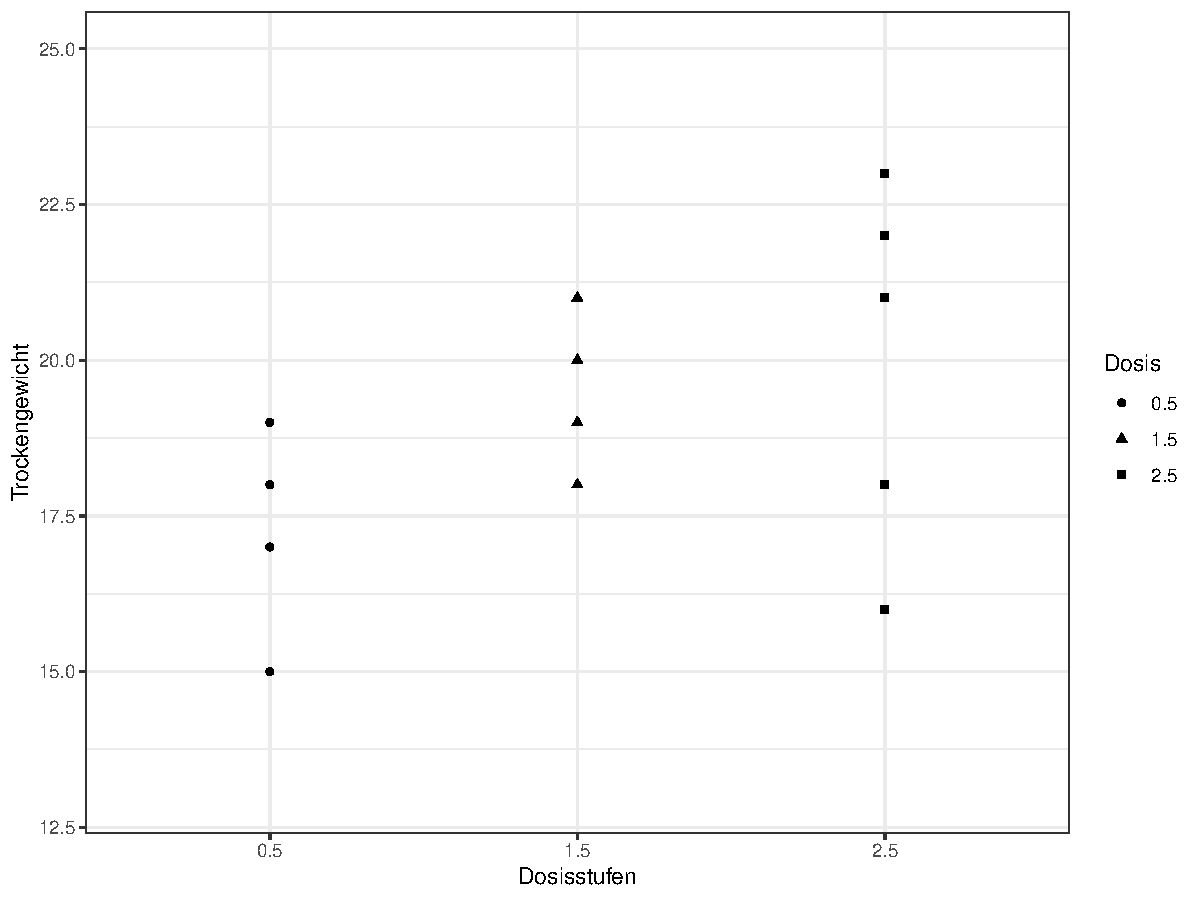
\includegraphics[width=\maxwidth]{img/anova-01-a-1} 

}


\end{knitrout}

\begin{enumerate}
\item Zeichnen Sie folgende statistischen Masszahlen in die Abildung ein! \textbf{(6 Punkte)}
  \begin{itemize}
  \item Total (grand) mean: $\beta_0$
  \item Mittelwerte der Dosen: $\bar{y}_{0.5}$, $\bar{y}_{1.5}$ und $\bar{y}_{2.5}$
  \item Effekt der einzelnen Level der Dosen: $\beta_{0.5}$, $\beta_{1.5}$,
    und $\beta_{2.5}$
  \item Residuen oder Fehler: $\epsilon$
  \end{itemize}
\item Sch{\"a}tzen Sie den p-Wert einer einfaktoriellen ANOVA ab. Liegt ein
  \textit{vermutlicher} signifikanter Unterschied zwischen den Dosisstufen
  vor? Begr{\"u}nden Sie Ihre Antwort! \textbf{(2 Punkte)}
\end{enumerate}
 
\clearpage
% -----------------------------------------------------------------------

\section{Aufgabe \hfill (13 Punkte)}


Der Datensatz \texttt{PlantGrowth} enth{\"a}lt das Gewicht der Pflanzen
(\textit{weight}), die unter einer Kontrolle und zwei verschiedenen
Behandlungsbedingungen erzielt wurden -- dem Faktor \textit{group} mit den
Faktorstufen \textit{ctrl}, \textit{trt1}, \textit{trt2}.



\begin{enumerate}
\item F{\"u}llen Sie die unterstehende einfaktorielle ANOVA Ergebnistabelle aus
  mit den gegebenen Informationen von \texttt{Df} und \texttt{Sum Sq}!
  \textbf{(4 Punkte)}
\item Sch{\"a}tzen Sie den p-Wert der Tabelle mit der Information von
  $F_{\alpha = 5\%} = 3.35$ ab. Begr{\"u}nden Sie Ihre
  Antwort! \textbf{(2 Punkte)}
\end{enumerate}

\vspace{1Ex}

\begin{center}
  \Large
  \begin{tabular}{l|c|c|c|c|c}
     & \textbf{Df} & \textbf{Sum Sq} & \textbf{Mean Sq} & \textbf{F value} & \textbf{Pr(>F)} \strut\\
    \hline
   \textbf{group}  & 2 & 3.84 &  &  &  \strut\\
    \hline
   \textbf{Residuals}  & 27 & 10.03 &  &  &  \strut\\
  \end{tabular}
\end{center}

\vspace{1Ex}

\begin{enumerate}
  \setcounter{enumi}{2}
\item Was bedeutet ein signifikantes Ergebnis in einer einfaktoriellen
  ANOVA im Bezug auf die m{\"o}glichen Unterschiede zwischen den Gruppen? Beziehen Sie sich auf den obigen Fragetext bei Ihrer Antwort!
  \textbf{(2 Punkte)}
\item Berechnen Sie \textit{einen} Student t-Test mit f{\"u}r den \textit{vermutlich}
  signifikantesten Gruppenvergleich anhand der untenstehenden Tabelle mit
  $T_{\alpha = 5\%} = 2.03$. Begr{\"u}nden Sie Ihre Auswahl! \textbf{(3 Punkte)}
\end{enumerate}

\begin{knitrout}
\definecolor{shadecolor}{rgb}{0.969, 0.969, 0.969}\color{fgcolor}\begin{table}[!h]
\centering
\begin{tabular}{cccc}
\toprule
group & n & mean & sd\\
\midrule
ctrl & 10 & 4.98 & 0.57\\
trt1 & 10 & 4.69 & 0.73\\
trt2 & 10 & 5.55 & 0.50\\
\bottomrule
\end{tabular}
\end{table}

\end{knitrout}

\begin{enumerate}
  \setcounter{enumi}{4}
\item Gegebenen der ANOVA Tabelle war das Ergebnis des t-Tests zu erwarten?
  Begr{\"u}nden Sie Ihre Antwort! \textbf{(2 Punkte)}
\end{enumerate}

 
\clearpage
% -----------------------------------------------------------------------

\section{Aufgabe \hfill (12 Punkte)}

Der Datensatz \textit{ToothGrowth} enth{\"a}lt Daten aus einer Studie zur
Bewertung der Wirkung von Vitamin C auf das Zahnwachstum bei
Meerschweinchen. Der Versuch wurde an 60 Schweinen durchgef{\"u}hrt, wobei
jedes Tier eine von drei Vitamin-C-Dosen \textit{dose} (0.5 mg/Tag, 1
mg/Tag und 2 mg/Tag) {\"u}ber eine von zwei Verabreichungsmethoden
\textit{supp} erhielt (Orangensaft oder Ascorbins{\"a}ure). Die Zahnl{\"a}nge wurde
als normalverteiltes Outcome gemessen.



\begin{enumerate}
\item F{\"u}llen Sie die unterstehende zweifaktorielle ANOVA Ergebnistabelle aus
  mit den gegebenen Informationen von \texttt{Df} und \texttt{Sum Sq}!
  \textbf{(4 Punkte)}
\item Sch{\"a}tzen Sie den p-Wert der Tabelle mit der Information von den
  kritischen F-Werten mit
  $F_{supp} = 4.02$ und
  $F_{dose} = 3.17$ sowie
  $F_{supp:dose} = 3.17$ ab. Begr{\"u}nden Sie Ihre
  Antwort! \textbf{(4 Punkte)}
\end{enumerate}

\vspace{1Ex}

\begin{center}
  \Large
  \begin{tabular}{l|c|c|c|c|c}
     & \textbf{Df} & \textbf{Sum Sq} & \textbf{Mean Sq} & \textbf{F value} & \textbf{Pr(>F)} \strut\\
    \hline
   \textbf{supp}  & 1 & 202.42 &  &  &  \strut\\
    \hline
    \textbf{dose}  & 2 & 2433.63 &  &  &  \strut\\
    \hline
    \textbf{supp:dose}  & 2 & 109.03 &  &  &  \strut\\
    \hline
   \textbf{Residuals}  & 54 & 713.5 &  &  &  \strut\\
  \end{tabular}
\end{center}

\vspace{1Ex}

\begin{enumerate}
  \setcounter{enumi}{2}
\item Was bedeutet ein signifikantes Ergebnis in einer zweifaktoriellen
  ANOVA im Bezug auf die m{\"o}glichen Unterschiede zwischen den Gruppen?
  Beziehen Sie sich dabei einmal auf den Faktor \textit{supp} und einmal
  auf den Faktor \textit{dose}! \textbf{(2 Punkte)}
\item Was sagt der Term \textit{supp:dose} aus? Interpretieren Sie das
  Ergebnis des abgesch{\"a}tzten p-Wertes! \textbf{(2 Punkte)}
\end{enumerate}
 
\clearpage
% -----------------------------------------------------------------------

\section{Aufgabe \hfill (8 Punkte)}


Der Datensatz \textit{Crop} enth{\"a}lt das Trockengewicht der
Maispflanzen (\textit{drymatter}), die unter drei 
verschiedenen D{\"u}ngerbedingungen erzielt wurden -- dem Faktor
\textit{trt} mit den Faktorstufen \textit{low}, \textit{mid},
\textit{high}. Sie erhalten folgenden Output in \Rlogo.

\begin{knitrout}
\definecolor{shadecolor}{rgb}{0.969, 0.969, 0.969}\color{fgcolor}\begin{kframe}
\begin{verbatim}
## Analysis of Variance Table
## 
## Response: drymatter
##           Df   Sum Sq  Mean Sq F value   Pr(>F)  
## trt        2  3.67455 1.837276 4.40437 0.022109 *
## Residuals 27 11.26301 0.417149                   
## ---
## Signif. codes:  0 '***' 0.001 '**' 0.01 '*' 0.05 '.' 0.1 ' ' 1
\end{verbatim}
\end{kframe}
\end{knitrout}

\begin{enumerate}
\item Stellen Sie die statistische $H_0$ und $H_A$ Hypothese f{\"u}r die obige
  einfaktorielle ANOVA auf! \textbf{(2 Punkte)}
\item Interpretieren Sie das Ergebnis der einfaktoriellen ANOVA! \textbf{(2 Punkt)} 
\item Berechen Sie den Effektsch{\"a}tzer $\eta^2$. Was sagt Ihnen der Wert von
  $\eta^2$ aus? \textbf{(2 Punkte)}
\item Skizieren Sie eine Abbildung, der dem obigen Ergebnis der
  einfaktoriellen ANOVA n{\"a}herungsweise entspricht! \textbf{(2 Punkte)}
\end{enumerate}

 
\clearpage
% -----------------------------------------------------------------------

\section{Aufgabe \hfill (8 Punkte)}



Der Datensatz \textit{PigGain} enth{\"a}lt Daten aus einer Studie zur Bewertung
der Wirkung vom Vitamin Selen auf das Wachstum bei Mastschweinen. Der
Versuch wurde an 64 Mastschweinen durchgef{\"u}hrt, wobei
jedes Tier eine von drei Selen-Dosen (0.5 ng/Tag, 1 ng/Tag und 5 ng/Tag)
{\"u}ber eine von zwei Verabreichungsmethoden erhielt (Wasser oder
Festnahrung). Sie erhalten folgenden Output in \Rlogo.

\begin{knitrout}
\definecolor{shadecolor}{rgb}{0.969, 0.969, 0.969}\color{fgcolor}\begin{kframe}
\begin{verbatim}
## Analysis of Variance Table
## 
## Response: len
##           Df   Sum Sq Mean Sq  F value                 Pr(>F)    
## supp       1  190.092 190.092 16.20122             0.00016724 ***
## dose       2 1878.817 939.408 80.06411 < 0.000000000000000222 ***
## supp:dose  2   83.583  41.791  3.56181             0.03475327 *  
## Residuals 58  680.526  11.733                                    
## ---
## Signif. codes:  0 '***' 0.001 '**' 0.01 '*' 0.05 '.' 0.1 ' ' 1
\end{verbatim}
\end{kframe}
\end{knitrout}

\begin{enumerate}
\item Stellen Sie die statistische $H_0$ und $H_A$ Hypothese f{\"u}r die obige
  zweifaktorielle ANOVA f{\"u}r den Faktor supp
  auf! \textbf{(2 Punkte)}
\item Interpretieren Sie das Ergebnis der zweifaktoriellen ANOVA. Gehen Sie
  im besonderen auf den Term $supp:dose$ ein! \textbf{(2 Punkte)}
\item Zeichnen Sie eine Abbildung, der dem obigen Ergebnis der
  zweifaktoriellen ANOVA n{\"a}herungsweise entspricht! \textbf{(4 Punkte)}
\end{enumerate}
 
\clearpage
% -----------------------------------------------------------------------

\section{Aufgabe \hfill (8 Punkte)}

In der untenstehenden Tabelle ist die Formel f{\"u}r den F-Test aus der ANOVA
und die Formel f{\"u}r den t-Test dargestellt. In der ANOVA berechnen Sie die
F-Statistik  $F_{calc}$ und in dem t-Test die T-Statistik  $T_{calc}$.

\begin{center}
  \begin{tabular}{cc}
    $F_{calc} = \cfrac{MS_{treatment}}{MS_{error}}$ & $T_{calc} = \cfrac{\bar{y}_1 - \bar{y}_2}{s_p \cdot \sqrt{2/n_g}}$\\
  \end{tabular}
\end{center}


\begin{enumerate}
\item Erkl{\"a}ren Sie den konzeptionellen Zusammenhang zwischen der $F_{calc}$
  Statistik und $T_{calc}$ Statistik! \textbf{(2 Punkte)}
\item Visualisieren Sie eine nicht signifikante $F_{calc}$ Statistik sowie
  eine signifikante $F_{calc}$ Statistik anhand von $MS_{treatment}$ und
  $MS_{error}$! Beschriften Sie die Abbildung! \textbf{(2 Punkte)}
\item Erkl{\"a}ren Sie an der Formel des F-Tests sowie an der Abbildung warum
  das Minimum der F-Statistik 0 ist! \textbf{(2 Punkte)}
\item Wenn die F-Statistik 0 ist, spricht dies eher f{\"u}r oder gegen die
  Nullhypothese? Beg{\"u}nden Sie Ihre Antwort! \textbf{(2 Punkte)}
\end{enumerate}

 
\clearpage
% -----------------------------------------------------------------------

\section{Aufgabe \hfill (6 Punkte)}

Sie rechnen eine zweifaktorielle ANOVA und erhalten einen signifikanten
Interaktionseffekt zwischen den beiden Faktoren $f_1$ und $f_2$. Der Faktor
$f_1$ hat drei Level. Der Faktor $f_2$ hat dagegen nur zwei Level.




\begin{enumerate}
\item Visualisieren Sie in zwei getrennten Abbildungen eine
  keine und eine schwache Interaktion zwischen
  den Faktoren $f_1$ und $f_2$! \textbf{(2 Punkte)}
\item Erkl{\"a}ren Sie den Unterschied zwischen den beiden St{\"a}rken der Interaktion!
  \textbf{(2 Punkte)}
\item Wenn eine signifikante Interaktion in den Daten vorliegt, wie ist
  dann das weitere Vorgehen bei einem Posthoc-Test?
  \textbf{(2 Punkte)}
\end{enumerate}

 
\clearpage
% -----------------------------------------------------------------------

\section{Aufgabe \hfill (7 Punkte)}



Sie rechnen eine einfaktorielle ANOVA mit einem Faktor $f_1$ mit
f{"u}nf Leveln. Nachdem Sie die einfaktorielle ANOVA gerechnet
haben, erhalten Sie einen p-Wert von $0.078$ und eine F Statistik mit
$F_{calc} = 1.2$. Als Sie sich die Boxplots der Behandlungen anschauen,
stellen Sie fest, dass es eigentlich einen Mittelwertsunterschied zwischen
dem zweiten und dritten Level geben m{\"u}sste. Die
$IQR$-Bereiche {\"u}berlappen sich nicht und die Mediane liegen auch weit vom
globalen Mittel entfernt.


\begin{enumerate}
\item Erkl{\"a}ren Sie die Annahme der Normalverteilung und die Annahme der
  Varianzhomogenit{\"a}t f{\"u}r eine ANOVA an einer passenden Abbildung! \textbf{(2 Punkte)}
\item Visualisieren Sie die Berechnung von $F_{calc}$ am obigen Beispiel!
  \textbf{(2 Punkte)}
\item Erkl{\"a}ren Sie das Ergebnis der obigen einfaktoriellen ANOVA unter der
  Ber{\"u}cksichtigung der Annahmen an eine ANOVA! \textbf{(3 Punkte)}
\end{enumerate}

 
\clearpage
% -----------------------------------------------------------------------

\section{Aufgabe \hfill (7 Punkte)}

Nach einem Gew{\"a}chshausexperiment mit drei Bew{\"a}sserungstypen ($low$, $mid$
und $high$) ergibt sich die folgende Datentabelle mit dem gemessenen
Frischgewicht (\textit{freshmatter}).

\begin{table}[!h]
\centering
\begin{tabular}{cc}
\toprule
water\_type & freshmatter\\
\midrule
low & 17\\
mid & 13\\
high & 19\\
high & 17\\
high & 19\\
\addlinespace
mid & 17\\
low & 19\\
low & 21\\
low & 20\\
high & 17\\
\addlinespace
mid & 21\\
low & 19\\
\bottomrule
\end{tabular}
\end{table}



\begin{enumerate}
\item Zeichnen Sie in \textit{einer} Abbildung die Barplots f{\"u}r die
  Bew{\"a}sserungstypen! Beschriften Sie die Achsen entsprechend!  \textbf{(4
    Punkte)}
\item Beschriften Sie \textit{einen} Barplot mit den g{\"a}ngigen
  statistischen Ma{\ss}zahlen! \textbf{(2 Punkte)}
\item Wenn Sie \textit{keinen Effekt} zwischen der Bew{\"a}sserungstypen
  erwarten w{\"u}rden, wie sehen dann die Barplots aus? \textbf{(1 Punkt)}
\end{enumerate} 
\clearpage
% -----------------------------------------------------------------------

\section{Aufgabe \hfill (9 Punkte)}

Nach einem Feldexperiment mit zwei D{\"u}ngestufen (A und B) ergibt sich die
folgende Datentabelle mit dem gemessenen Trockengewicht (\textit{drymatter}). 

\begin{table}[!h]
\centering
\begin{tabular}{cc}
\toprule
trt & drymatter\\
\midrule
B & 17.1\\
B & 18.3\\
B & 22.3\\
B & 3.6\\
A & 10.6\\
\addlinespace
A & 5.7\\
A & 9.1\\
A & 15.0\\
B & 15.1\\
A & 12.2\\
\addlinespace
B & 14.9\\
B & 11.9\\
A & 14.6\\
A & 12.2\\
B & 12.9\\
\addlinespace
A & 11.1\\
B & 20.0\\
B & 12.3\\
A & 6.9\\
A & 11.3\\
\addlinespace
A & 13.4\\
B & 18.6\\
\bottomrule
\end{tabular}
\end{table}



\begin{enumerate}
\item Zeichnen Sie in \textit{einer} Abbildung die beiden Boxplots f{\"u}r die
  zwei D{\"u}ngestufen A und B! Beschriften Sie die Achsen entsprechend!
  \textbf{(6 Punkte)}
\item Beschriften Sie \textit{einen} der beiden Boxplots mit den g{\"a}ngigen
  statistischen Ma{\ss}zahlen! \textbf{(2 Punkte)}
\item Wenn Sie \textit{keinen Effekt} zwischen den D{\"u}ngestufen erwarten
  w{\"u}rden, wie sehen dann die beiden Boxplots aus? \textbf{(1 Punkt)}
\end{enumerate} 
\clearpage
% -----------------------------------------------------------------------

\section{Aufgabe \hfill (9 Punkte)}

Nach einem Feldexperiment mit mehreren D{\"u}ngestufen stellt sich die Frage,
ob die D{\"u}ngestufe \textit{low} im Bezug auf das Trockengewicht
normalverteilt sei. Sie erhalten folgende Datentabelle.

\begin{table}[!h]
\centering
\begin{tabular}{cc}
\toprule
fertilizer & drymatter\\
\midrule
low & 14\\
low & 16\\
low & 11\\
low & 22\\
low & 19\\
\addlinespace
low & 16\\
low & 16\\
\bottomrule
\end{tabular}
\end{table}



\begin{enumerate}
\item Zeichnen Sie eine passende Abbildung in der Sie visuell {\"u}berpr{\"u}fen
  k{\"o}nnen, ob eine Normalverteilung des Trockengewichts vorliegt! \textbf{(4
    Punkte)}
\item Beschriften Sie die Achsen und erg{\"a}nzen Sie die statistischen
  Ma{\ss}zahlen. \textbf{(3 Punkte)}
\item Entscheiden Sie, ob eine Normalveteilung vorliegt. Begr{\"u}nden Sie Ihre
  Antwort. \textbf{(2 Punkte)}
\end{enumerate} 
\clearpage
% -----------------------------------------------------------------------

\section{Aufgabe \hfill (4 Punkte)}



\begin{enumerate}
\item Zeichnen Sie {\"u}ber den untenstehenden Boxplot die entsprechende
  zugeh{\"o}rige Verteilung! \textbf{(2 Punkte)} 
\item Zeichnen Sie unter den untenstehenden Boxplot die entsprechende
  zugeh{\"o}rige Beobachtungen! \textbf{(2 Punkte)}
\end{enumerate}

\vspace*{8cm}

\begin{center}
  
\includegraphics[width=10cm]{/Users/kruppajo/Documents/GitHub/exam/question/img/boxplot-03-b.png}
\end{center}



 
\clearpage
% -----------------------------------------------------------------------

\section{Aufgabe \hfill (10 Punkte)}



Nach einem Experiment ergibt sich die folgende 2x2 Datentabelle mit einem
Pestizid (ja/nein), dargestellt in den Zeilen. Im Weiteren mit dem
infizierten Pflanzenstatus (ja/nein) in den Spalten. Insgesamt wurden
$n = 114$ Pflanzen untersucht.
\vspace{5Ex}

\begin{center}
  \Large
  \begin{tabular}{c|c|c|c}
     & \textbf{Erkrankt (ja)} & \textbf{Erkrankt (nein)} &  \strut\\
    \hline
    \textbf{Pestizid (ja)} & 24  & 11  &     \strut\\
    \hline
    \textbf{Pestizid (nein)} & 27  & 52  &      \strut\\
    \hline
     \phantom{100} & \phantom{100}  & \phantom{100}  &  \phantom{100}  \strut\\
  \end{tabular}
\end{center}

\vspace{5Ex}

\begin{enumerate}
\item Erg{\"a}nzen Sie die Tabelle um die Randsummen! \textbf{(1 Punkt)} 
\item Formulieren Sie die Fragestellung! \textbf{(1 Punkt)}
\item Formulieren Sie das Hypothesenpaar! \textbf{(2 Punkte)}
\item Berechnen Sie die Teststatistik eines Chi-Quadrat-Test auf der 2x2
  Tafel. Geben Sie Formeln und Rechenweg mit an! \textbf{(4 Punkte)}
\item Treffen Sie eine Entscheidung im Bezug zu der Nullhypothese gegeben
  einem $T_k = 3.841$! \textbf{(1 Punkt)}
\item Skizzieren Sie eine 2x2 Tabelle mit
  $n = 30$ Pflanzen in dem \textit{vermutlich}
  die Nullhypothese nicht abgelehnt werden kann! \textbf{(1 Punkt)}
\end{enumerate} 
\clearpage
% -----------------------------------------------------------------------

\section{Aufgabe \hfill (7 Punkte)}



Gegeben sind folgende Randsummen in einer 2x2 Kreuztabelle aus einem
Experiment mit $n = 153$ Sauen. In dem Experiment wurde gemessen,
ob eine Sau nach einer Behandlung mit einem Medikament (ja/nein)
mehr als 30 Ferkel pro Jahr bekommen konnte (ja/nein).

\vspace{5Ex}

\begin{center}
  \Large
  \begin{tabular}{c|c|c|c}
     & \textbf{>30 Ferkel (ja)} & \textbf{$\leq$30 Ferkel (nein)} &  \strut\\
    \hline
    \textbf{Medikament (ja)} & \phantom{100}  & \phantom{100}  &   68  \strut\\
    \hline
    \textbf{Medikament (nein)} & \phantom{100}  & \phantom{100}  &   85   \strut\\
    \hline
     &  96 &  57 &  153  \strut\\
  \end{tabular}
\end{center}



\vspace{5Ex}

\begin{enumerate}
\item Erg{\"a}nzen Sie die Felder innerhalb der 2x2 Kreuztabelle in dem Sinne,
  dass \textit{kein} signifikanter Effekt zu erwarten w{\"a}re!
  \textbf{(2 Punkte)}
\item Erkl{\"a}ren und Begr{\"u}nden Sie Ihr Vorgehen an der Formel des
  Chi-Quadrat-Tests mit
  \begin{equation*}
  \mathcal{X}^2 = \sum\tfrac{(O - E)^2}{E}.  
  \end{equation*}
  Sie k{\"o}nnen dies an einem Beispiel erkl{\"a}ren! \textbf{(2 Punkte)}
\item Was ist die Mindestanzahl an Beobachtungen je Zelle? Wenn in einer
  der Zellen weniger Beobachtungen auftreten, welchen Test k{\"o}nnen Sie
  anstatt des "`normalen"' Chi-Quadrat-Tests anwenden? \textbf{(2 Punkte)}
\item Warum hat die obige Vierfeldertafel einen Freiheitsgrad von $df=1$?
  \textbf{(1 Punkt)}
\end{enumerate} 
\clearpage
% -----------------------------------------------------------------------

\section{Aufgabe \hfill (9 Punkte)}

Im folgenden sehen Sie drei leere Scatterplots. F{\"u}llen Sie diese
Scatterplots nach folgenden Anweisungen.

\begin{enumerate}
\item Zeichnen Sie f{\"u}r die angegebene $\rho$-Werte eine Gerade in die
  entsprechende Abbildung! \textbf{(3 Punkte)}
\item Zeichnen Sie f{\"u}r die angegebenen $R^2$-Werte die entsprechende
  Punktewolke um die Gerade. \textbf{(3 Punkte)}
\item Sie rechnen ein statistisches Modell. Was sagen Ihnen die $R^2$-Werte
  {\"u}ber das jeweilige Modell? \textbf{(3 Punkte)}
\end{enumerate}




{\centering 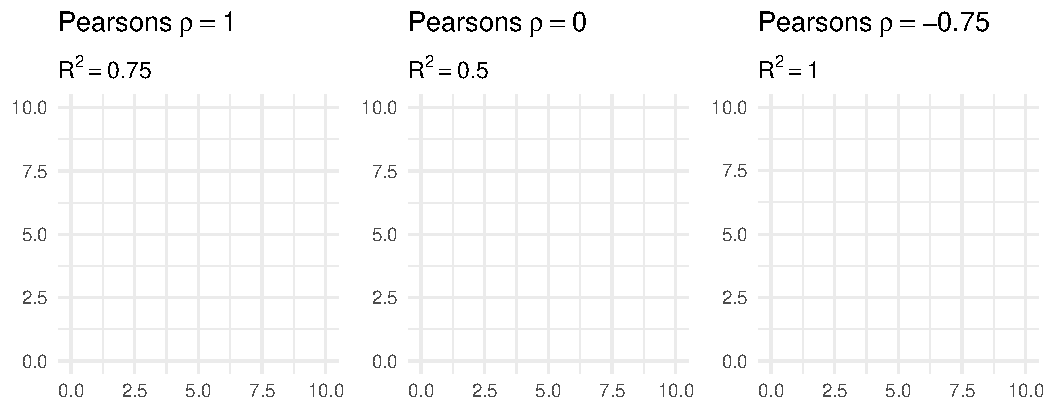
\includegraphics[width=\maxwidth]{img/correlation-01-1} 

}



 
\clearpage
% -----------------------------------------------------------------------

\section{Aufgabe \hfill (10 Punkte)}

Im folgenden sehen Sie vier Scatterplots. Erg{\"a}nzen Sie die {\"U}berschriften
der jeweiligen Scatterplots.


\begin{enumerate}
\item Sch{\"a}tzen Sie die $\rho$-Werte in der entsprechenden
  Abbildung! \textbf{(4 Punkte)}
\item Sch{\"a}tzen Sie die $R^2$-Werte in der entsprechenden
  Punktewolke um die Gerade! \textbf{(4 Punkte)}
\item Sie rechnen ein statistisches Modell. Was sagen Ihnen die $R^2$-Werte
  {\"u}ber das jeweilige Modell? \textbf{(2 Punkte)}
\end{enumerate}




{\centering 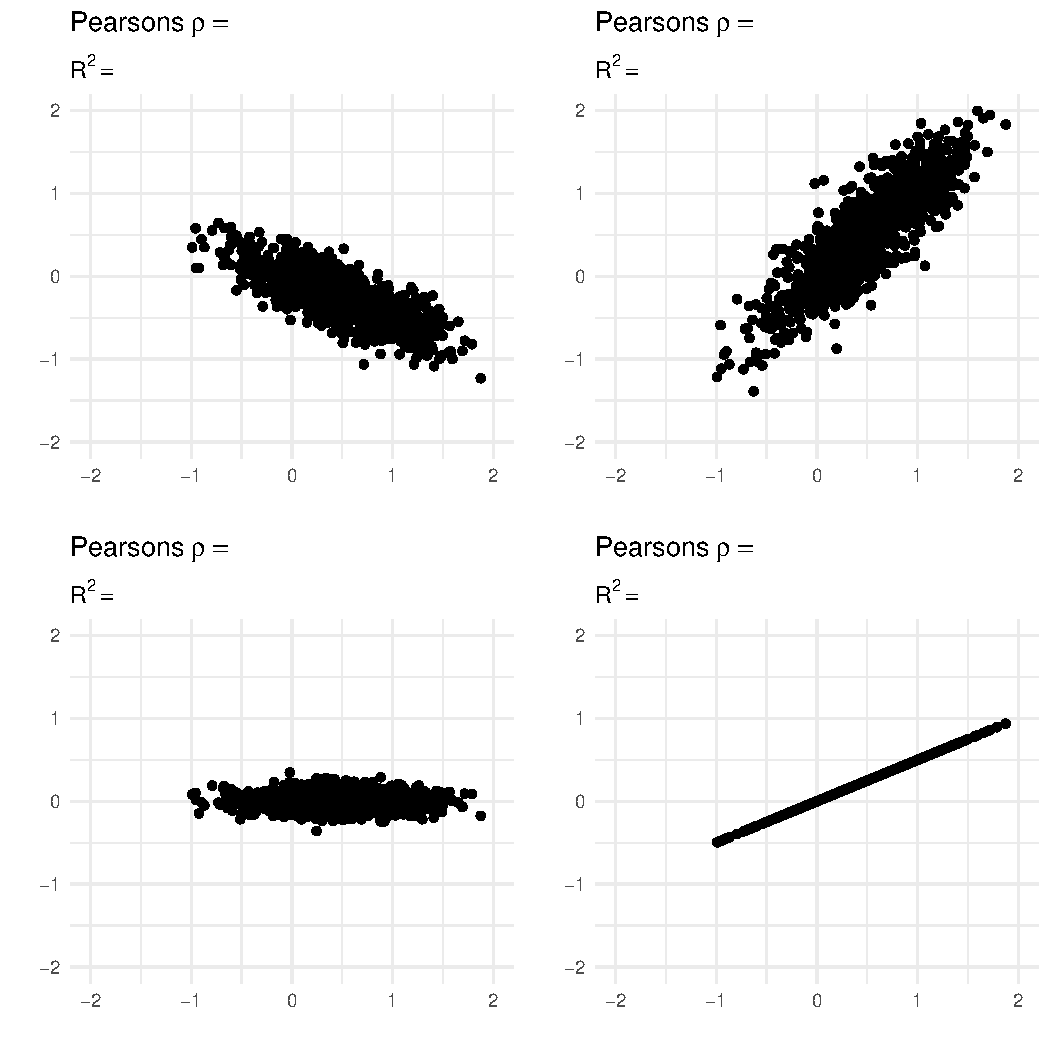
\includegraphics[width=\maxwidth]{img/correlation-02-1} 

}



 
\clearpage
% -----------------------------------------------------------------------

\section{Aufgabe \hfill (8 Punkte)}

Sie haben folgende Zahlenreihe $y$ vorliegen
$y = \{16, 15, 12, 15, 13, 13\}$.

\begin{enumerate}
\item Visualisieren Sie den Mittelwert von $y$ in der untenstehenden
  Abbildung! \textbf{(4 Punkte)}
\item Beschriften Sie die $Y$ und $X$-Achse entsprechend! \textbf{(2 Punkte)}
\item F{\"u}r die Berechnung der Varianz wird der Abstand der einzelnen Werte $x_i$
  zum Mittelwert $\bar{x}$ quadriert. Warum muss der Abstand, $x_i -
  \bar{x}$, in der Varianzformel quadriert werden?
  Erkl{\"a}ren Sie den Zusammenhang unter Ber{\"u}cksichtigung der Abbildung!
  \textbf{(2 Punkte)}  
\end{enumerate}



{\centering 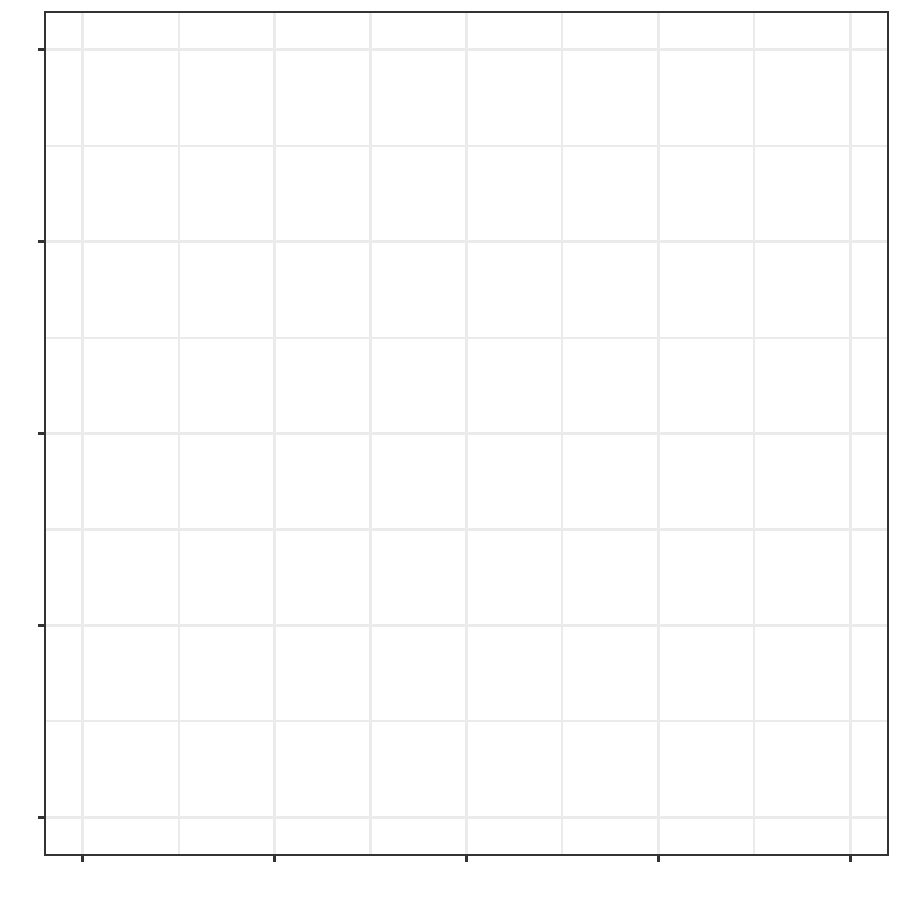
\includegraphics[width=\maxwidth]{img/desc-01-1} 

}


 
\clearpage
% -----------------------------------------------------------------------

\section{Aufgabe \hfill (10 Punkte)}

Sie haben folgende Zahlenreihe $y$ vorliegen
$y = \{12, 17, 19, 15, 14, 23, 16\}$. Berechnen Sie folgende
deskriptive Ma{\ss}zahlen. Geben Sie Formeln und Rechenwege mit an!



\begin{enumerate}
\item Das 3rd Quartile \textbf{(2 Punkte)}
\item Die Range oder Spannweite \textbf{(2 Punkte)}
\item Das 1st Quartile \textbf{(2 Punkte)}
\item Die Standardabweichung \textbf{(2 Punkte)}
\item Den Mittelwert \textbf{(2 Punkte)}
\end{enumerate}
 
\clearpage
% -----------------------------------------------------------------------

\section{Aufgabe \hfill (11 Punkte)}

Die Pr{\"a}valenz von Klauenseuche bei Wollschweinen wird mit
3\% angenommen. In 85\% der F{\"a}lle ist ein Test positiv, wenn das Wollschwein erkrankt
ist. In 7.5\% der F{\"a}lle ist ein Test positiv,
wenn das Wollschwein \textit{nicht} erkrankt ist und somit gesund ist. Sie
werten 1000 Wollschweine mit einem
diagnostischen Test auf Klauenseuche aus.



\begin{enumerate}
\item F{\"u}llen und beschriften Sie den untenstehenden Doppelbaum! Beschriften
  Sie auch die {\"A}ste des Doppelbaumes, mit denen Ihnen bekannten
  Informationen!  \textbf{(8 Punkte)}
\item Berechnen Sie die Wahrscheinlichkeit $Pr(K^+|T^+)$! \textbf{(2 Punkte)}
\item Was sagt Ihnen die Wahrscheinlichkeit $Pr(K^+|T^+)$ aus? \textbf{(1 Punkt)}
\end{enumerate}

\vspace{1cm}

\begin{center}
  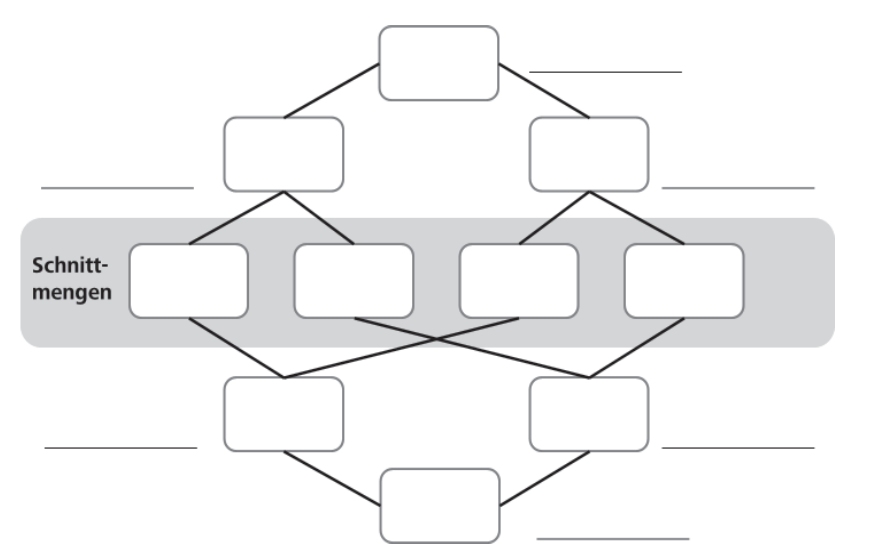
\includegraphics[width=17cm]{/Users/kruppajo/Documents/GitHub/exam/question/img/diag-doppelbaum}
\end{center}



 
\clearpage
% -----------------------------------------------------------------------

\section{Aufgabe \hfill (9 Punkte)}

Beim diagnostischen Testen erhalten Sie \textit{True Positives (TP)},
\textit{True Negatives (TN)}, \textit{False Positives (FP)} und
\textit{False Negatives (FN)}. Erkl{\"a}ren Sie den Zusammenhang wir folgt.

\begin{enumerate}
\item Visualisieren Sie \textit{TP}, \textit{TN}, \textit{FP} und
  \textit{FN} in einer Abbildung. Beschriften Sie die Abbildung und die
  Achsen entsprechend! \textbf{(6 Punkte)}
\item Tragen Sie \textit{TP}, \textit{TN}, \textit{FP} und \textit{FN} in
  eine 2x2 Kreuztablle ein. Beschriften Sie die Tabelle entsprechend!
  \textbf{(3 Punkte)}
\end{enumerate}





 
\clearpage
% -----------------------------------------------------------------------

\section{Aufgabe \hfill (12 Punkte)}



Folgender diagnostischer Doppelbaum nach der Testung auf Klauenseuche bei
Fleckvieh ist gegeben.

\begin{enumerate}
\item F{\"u}llen und beschriften Sie den untenstehenden Doppelbaum! \textbf{(4
    Punkte)}
\item Berechnen Sie die Wahrscheinlichkeit $Pr(K^+|T^+)$! \textbf{(2 Punkte)}
\item Berechnen Sie die Pr{\"a}valenz f{\"u}r Klauenseuche! \textbf{(2 Punkte)}
\item Berechnen Sie die Sensifit{\"a}t und Spezifit{\"a}t des diagnostischen Tests
  f{\"u}r Klauenseuche! Erstellen Sie daf{\"u}r zun{\"a}chst eine 2x2 Kreuztabelle aus
  dem ausgef{\"u}llten Doppelbaum!
  \textbf{(4 Punkte)}
\end{enumerate}

\vspace{1cm}
 
\begin{tikzpicture}
  \node (image) at (0,0) {
    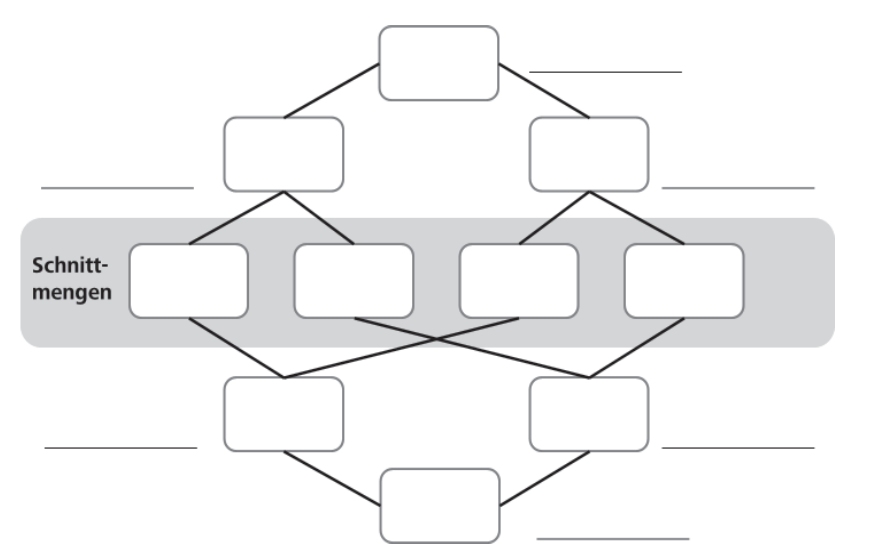
\includegraphics[width=\textwidth]{/Users/kruppajo/Documents/GitHub/exam/question/img/diag-doppelbaum}
  };
  \node[] at (-4.8,0) {\huge 180};
  \node[] at (-1.7,0) {\huge 40};
  \node[] at (1.7,0) {\huge 750};
  \node[] at (4.75,0) {\huge 1800};
\end{tikzpicture}




 
\clearpage
% -----------------------------------------------------------------------

\section{Aufgabe \hfill (6 Punkte)}

Nach einer Bonitur von Schnittlauch mit einer Kontrolle und drei Pestiziden (ctrl, pestKill, roundUp, zeroX) ergibt sich die folgende Datentabelle mit den Boniturnoten (\textit{grade}). 

\begin{table}[!h]
\centering
\begin{tabular}{cc}
\toprule
pesticide & grade\\
\midrule
pestKill & 4\\
ctrl & 8\\
ctrl & 5\\
pestKill & 4\\
pestKill & 4\\
\addlinespace
roundUp & 5\\
zeroX & 3\\
ctrl & 5\\
roundUp & 5\\
zeroX & 1\\
\addlinespace
roundUp & 6\\
zeroX & 2\\
pestKill & 1\\
roundUp & 6\\
\bottomrule
\end{tabular}
\end{table}



\begin{enumerate}
\item Zeichnen Sie in \textit{einer} Abbildung die Dotplots f{\"u}r die
  vier Pestizidlevel! Beschriften Sie die Achsen entsprechend!
  \textbf{(3 Punkte)}
\item Erg{\"a}nzen Sie die Dotplots mit den g{\"a}ngigen
  statistischen Ma{\ss}zahlen. \textbf{(2 Punkte)}
\item Wenn Sie \textit{keinen Effekt} zwischen den Pestizidlevel erwarten
  w{\"u}rden, wie sehen dann die Dotplots aus? \textbf{(1 Punkt)}
\end{enumerate} 
\clearpage
% -----------------------------------------------------------------------

\section{Aufgabe \hfill (6 Punkte)}



\begin{enumerate}
\item Skizieren Sie in die unten stehenden, freien Abbildungen die
  Verteilungen, die sich nach der Abbilungs{\"u}berschrift ergeben! \textbf{(4
    Punkte)}
\item Achten Sie auf die entsprechende Skalierung der beiden Verteilungen
  in der ersten Abbildung! \textbf{(2 Punkte)}
\end{enumerate}



{\centering 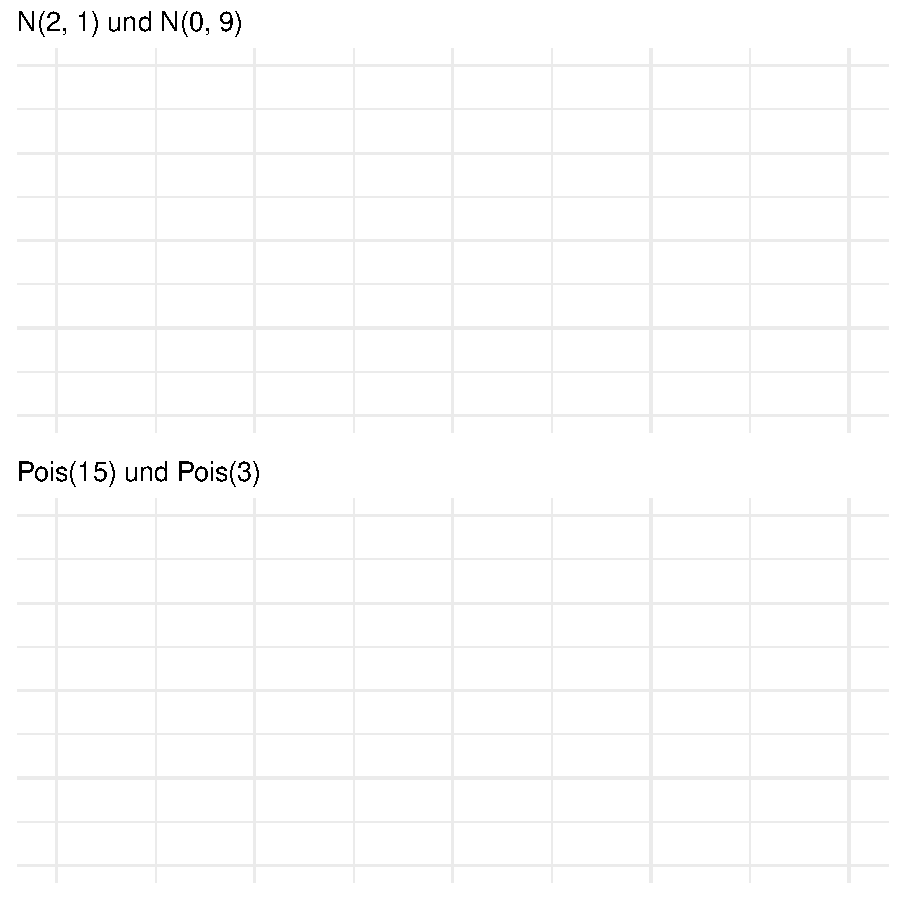
\includegraphics[width=\maxwidth]{img/histogram-01-1} 

}



 
\clearpage
% -----------------------------------------------------------------------

\section{Aufgabe \hfill (6 Punkte)}



\begin{enumerate}
\item Skizieren Sie $4$ Normalverteilungen \textit{in einer
    Abbildung} mit $\mu_1 \neq \mu_2 \neq \mu_3 \neq \mu_4$ und $s_1 = s_2 = s_3 = s_4$! \textbf{(2 Punkte)}
\item Beschriften Sie die Normalverteilungen mit den entsprechenden
  Parametern! \textbf{(2 Punkte)}
\item Liegt Varianzhomogenit{\"a}t oder Varianzheterogenit{\"a}t vor? Begr{\"u}nden Sie
  Ihre Antwort! \textbf{(2 Punkte)}
\end{enumerate}

 
\clearpage
% -----------------------------------------------------------------------

\section{Aufgabe \hfill (6 Punkte)}



Nach einem Experiment z{\"a}hlen Sie folgende Anzahl an L{\"a}sionen auf den
Bl{\"a}ttern von Sonnenblumen nach einer durchgestandenen Infektion. 

\begin{center}
$3, 4, 4, 1, 9, 1, 2, 5, 2, 7, 7, 3$
\end{center}

\begin{enumerate}
\item Zeichen Sie ein Histogramm um die Verteilung der Daten zu visualiseren. (\textbf{3 Punkte})
\item Beschriften Sie die Achsen der Abbildung! (\textbf{2 Punkte})
\item Erg{\"a}nzen Sie die relativen H{\"a}ufigkeiten in der Abbildung! \textbf{1 Punkt}
\end{enumerate}

 
\clearpage
% -----------------------------------------------------------------------

\section{Aufgabe \hfill (6 Punkte)}



\begin{enumerate}
\item Skizieren Sie in die unten stehenden, freien Abbildungen ein kausales
  und ein pr{\"a}diktives Modell mit $n = 9$
  Beobachtungen! \textbf{(4 Punkte)}
\item Beachten Sie bei der Erstellung der Skizze, ob ein Effekt von X
  vorliegt oder nicht! \textbf{(2 Punkte)}
\end{enumerate}



{\centering 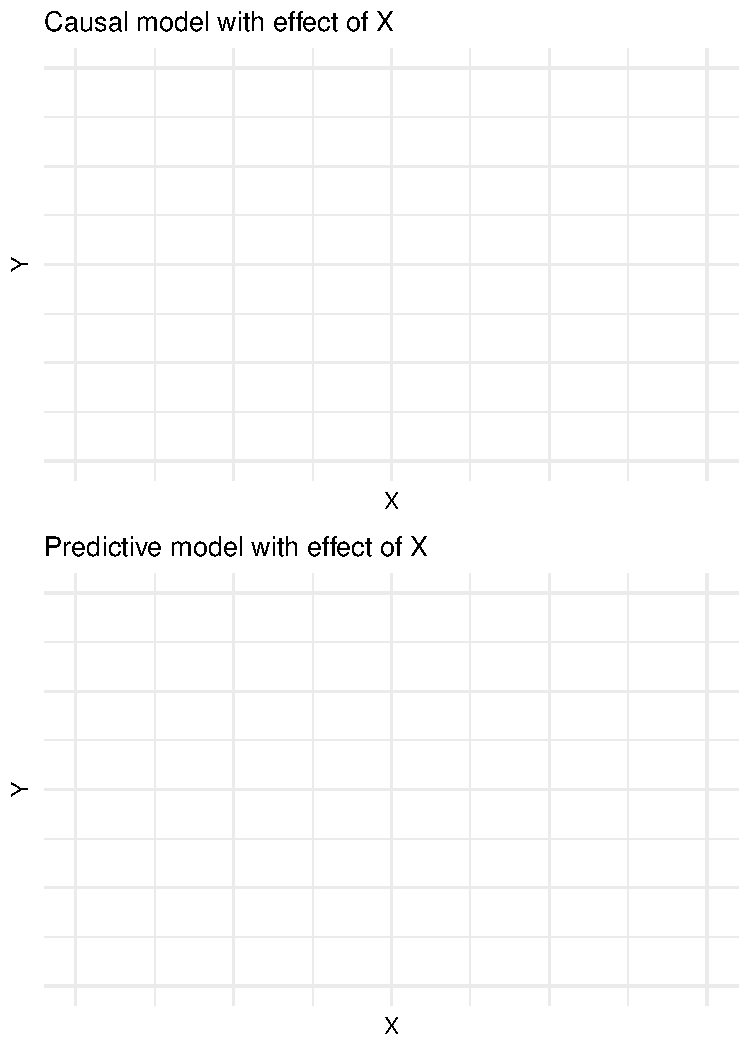
\includegraphics[width=\maxwidth]{img/modeling-01-1} 

}



 
\clearpage
% -----------------------------------------------------------------------

\section{Aufgabe \hfill (9 Punkte)}



Ein Feldexperiment wurde mit $n = 200$ Pflanzen durchgef{\"u}hrt. Folgende
Einflussvariablen ($x$) wurden erhoben: rainfall, S und N. Als m{\"o}gliche Outcomevariablen stehen Ihnen nun
folgende gemessene Endpunkte zu Verf{\"u}gung: drymatter, yield, count, quality\_score und dead.

\begin{enumerate}
\item W{\"a}hlen Sie ein Outcome was zu der Verteilungsfamilie
  \textit{Gaussian} geh{\"o}rt! \textbf{(1 Punkt)}
\item Schreiben Sie das Modell in der Form $y \sim x$ wie es in \Rlogo
  {\"u}blich ist \textit{ohne Interaktionsterm}! \textbf{(2 Punkte)}
\item Schreiben Sie das Modell in der Form $y \sim x$ wie es in \Rlogo
  {\"u}blich ist und erg{\"a}nzen Sie \textit{einen} Interaktionsterm nach Wahl! \textbf{(2 Punkte)} 
\item Zeichen Sie eine \textit{schwache}
  Interaktion in die Abbildung unten f{\"u}r den Endpunkt
  \textit{yield}. Erg{\"a}nzen Sie eine aussagekr{\"a}ftige Legende. Wie erkennen
  Sie eine Interaktion? Begr{\"u}nden Sie Ihre Antwort! \textbf{(4 Punkte)}
\end{enumerate}



{\centering 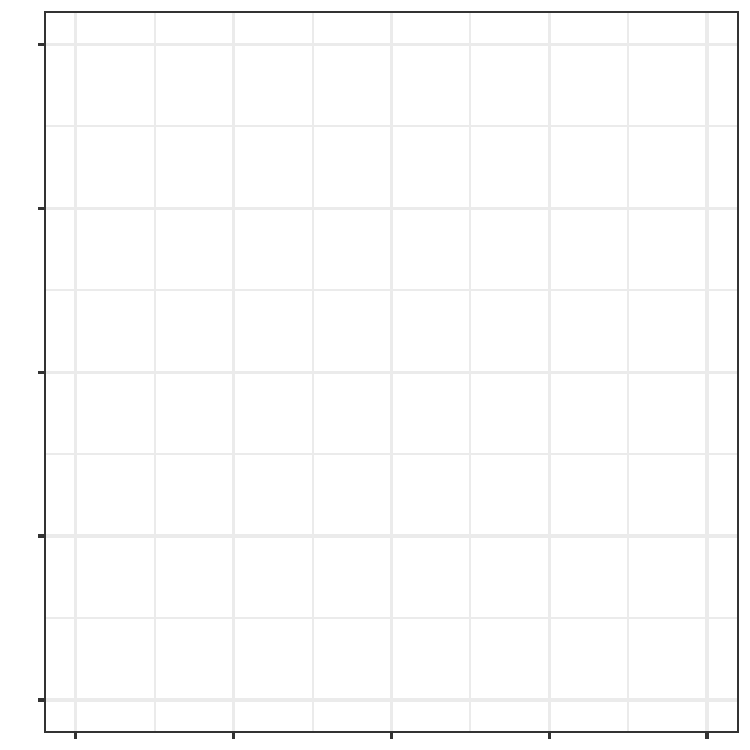
\includegraphics[width=\maxwidth]{img/modeling-R-01-1} 

}


 
\clearpage
% -----------------------------------------------------------------------

\section{Aufgabe \hfill (6 Punkte)}

Nach einem Feldexperiment mit zwei Pestiziden (\textit{RoundUp} und
\textit{OutEx}) ergibt sich die folgende Datentabelle mit dem jeweiligen
beobachteten Infektionsstatus.

\begin{table}[!h]
\centering
\begin{tabular}{cc}
\toprule
pesticide & infected\\
\midrule
OutEx & no\\
OutEx & no\\
OutEx & no\\
RoundUp & no\\
RoundUp & no\\
\addlinespace
RoundUp & no\\
OutEx & no\\
OutEx & no\\
RoundUp & yes\\
RoundUp & no\\
\addlinespace
OutEx & no\\
OutEx & no\\
OutEx & no\\
RoundUp & yes\\
RoundUp & no\\
\addlinespace
RoundUp & no\\
RoundUp & yes\\
OutEx & yes\\
RoundUp & yes\\
OutEx & no\\
\addlinespace
RoundUp & no\\
OutEx & yes\\
\bottomrule
\end{tabular}
\end{table}



\begin{enumerate}
\item Stellen Sie in einer 2x2 Tafel den Zusammenhang zwischen dem
  Pesizid und dem Infektionsstatus dar! \textbf{(2 Punkte)}
\item Zeichnen Sie den zugeh{\"o}rigen Mosaic-Plot. Berechnen Sie das
  Verh{\"a}ltnis pro Spalte! \textbf{(2 Punkte)}
\item Wenn das Pesizid keine Auswirkung auf den Infektionsstatus h{\"a}tte, wie
  sehe dann der Mosaic-Plot aus? \textbf{(2 Punkte)}
\end{enumerate} 
\clearpage
% -----------------------------------------------------------------------

\section{Aufgabe \hfill (6 Punkte)}

In einem Experiment zur Dosiswirkung wurden verschiedene Dosisstufen mit
einer Kontrollgruppe vergleichen. Es wurden vier t-Test f{\"u}r den
Mittelwertsvergleich gerechnet und es ergab sich folgende Tabelle mit den
rohen p-Werten.



\begin{center}
  \Large
  \begin{tabular}{c|c|c|c}
    \textbf{Vergleich} & \textbf{Raw p-val} & \textbf{Adjusted p-val} &
                                                                        \textbf{Reject $\boldsymbol{H_0}$} \strut\\
    \hline
    dose 10 - ctrl  & 0.020 &  &\strut\\
    \hline
    dose 15 - ctrl  & 0.060 & &\strut\\
    \hline
    dose 20 - ctrl  & 0.001 & &\strut\\
    \hline
    dose 40 - ctrl  & 0.012 & &\strut\\
  \end{tabular}
\end{center}

\begin{enumerate}
\item F{\"u}llen Sie die Spalte "`adjustierte p-Werte"' mit den adjustierten
  p-Werten nach Bonferoni aus! \textbf{(2 Punkte)}
\item Entscheiden Sie, ob nach der Adjustierung die Nullhypothese weiter
  abglehnt werden kann. Tragen Sie Ihre Entscheidung in die obige Tabelle
  ein. Begr{\"u}nden Sie Ihre Antwort! \textbf{(2 Punkte)}
\item Erkl{\"a}ren Sie warum die p-Werte bei multiplen Vergleichen
  adjustiert werden m{\"u}ssen? \textbf{(2 Punkte)}
\end{enumerate}

\vspace{1Ex}

 
\clearpage
% -----------------------------------------------------------------------

\section{Aufgabe \hfill (10 Punkte)}



\begin{enumerate}
\item Zeichen Sie in die drei untenstehenden, leeren Abbilungen die Zeile des
  Regressionskreuzes der Binomialverteilung. W{\"a}hlen Sie die Beschriftung der
  y-Achse sowie der x-Achse entsprechend aus! \textbf{(6 Punkte)}
\item Welchen Effektsch{\"a}tzer erhalten Sie aus der entsprechend linearen
  Regression? Geben Sie ein Beispiel! \textbf{(2 Punkte)}
\item Wenn Sie keinen Effekt erwarten, welchen \textit{Zahlenraum} nimmt dann
  der Effektsch{\"a}tzer ein? Geben Sie ein Beispiel! \textbf{(2 Punkte)}
\end{enumerate}



{\centering 
\includegraphics[width=\maxwidth]{img/regression-01-1} 

}



 
\clearpage
% -----------------------------------------------------------------------

\section{Aufgabe \hfill (10 Punkte)}



In einem Stallexperiment mit $n = 92$ Ferkeln wurde der
Gewichtszuwachs unter bestimmten Lichtverh{\"a}ltnissen gemessen. Sie erhalten
den \Rlogo Output der Funktion \texttt{tidy()} einer simplen Gaussian linearen
Regression sieben Wochen nach der ersten Messung.

\begin{table}[!h]
\centering\begingroup\fontsize{14}{16}\selectfont

\begin{tabular}{ccccc}
\toprule
term & estimate & std.error & t statistic & p-value\\
\midrule
(Intercept) & 23.58 & 1.25 &  & \\
light & 1.66 & 0.12 &  & \\
\bottomrule
\end{tabular}
\endgroup{}
\end{table}



\begin{enumerate}
\item Berechnen Sie die t Statistik f{\"u}r \textit{(Intercept)} und
  \textit{light}! \textbf{(2 Punkte)}
\item Sch{\"a}tzen Sie den p-Wert f{\"u}r \textit{(Intercept)} und
  \textit{light} mit $T_k = 1.96$ ab. Was sagt Ihnen der p-Wert aus?
  Begr{\"u}nden Sie Ihre Antwort! \textbf{(3 Punkte)}
\item Zeichnen Sie die Gerade aus der obigen Tabelle in die untenstehende
  Abbildung! \textbf{(1 Punkt)}
\item Beschriften Sie die Abbildung und die Gerade mit den statistischen
  Kenngr{\"o}{\ss}en! \textbf{(2 Punkte)}
\item Formulieren Sie die Regressionsgleichung! \textbf{(2 Punkte)}
\end{enumerate}



{\centering 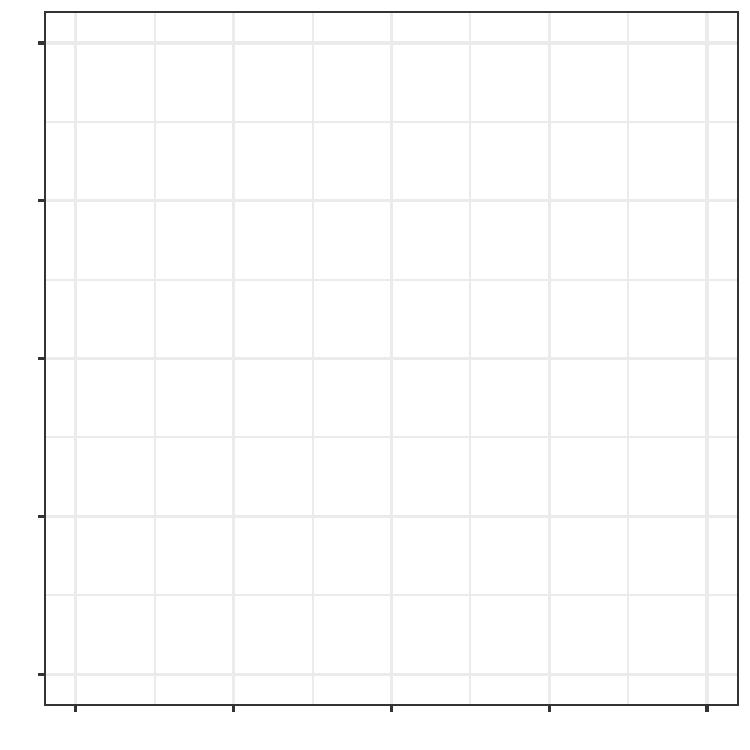
\includegraphics[width=\maxwidth]{img/regression-02-b-1} 

}


 
\clearpage
% -----------------------------------------------------------------------

\section{Aufgabe \hfill (4 Punkte)}



\begin{enumerate}
\item Skizieren Sie in die unten stehende, freie Abbildung die
  Abbildung, die sich nach der {\"U}berschrift ergibt! \textbf{(2 Punkte)}
\item Beschriften Sie die Achsen entsprechend! \textbf{(2 Punkte)}
\end{enumerate}



{\centering 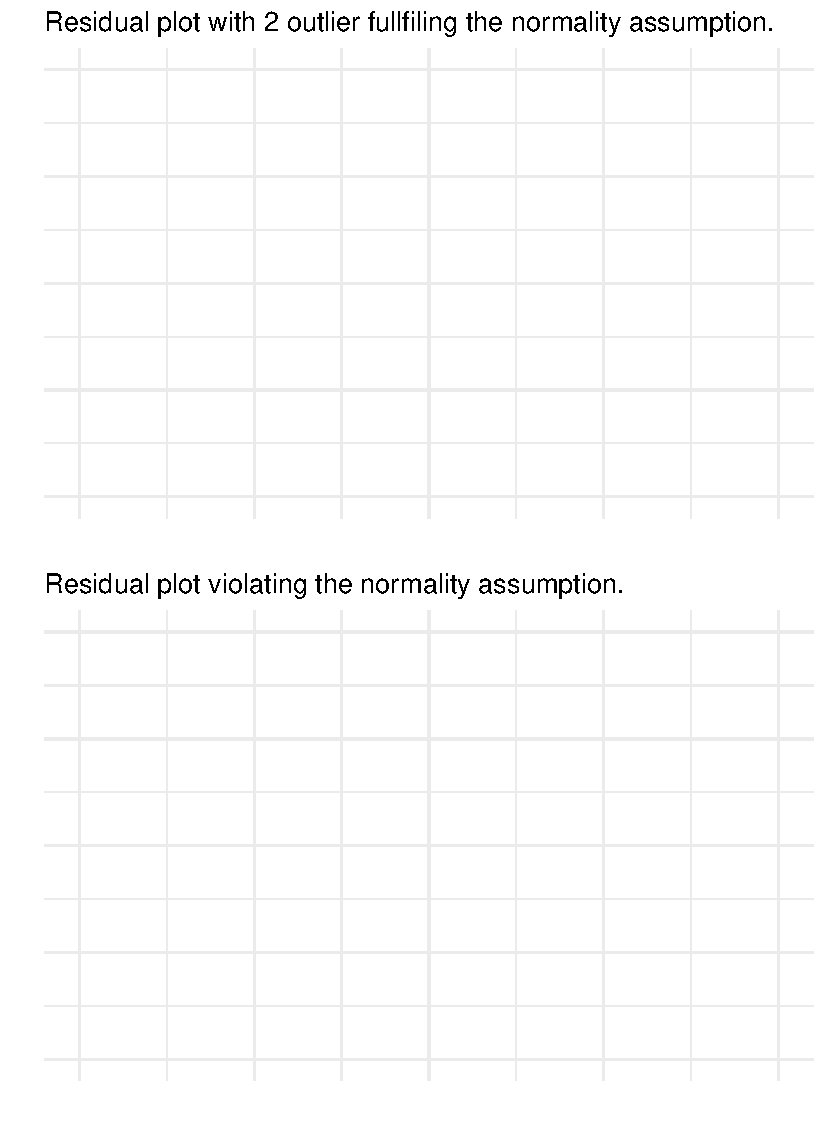
\includegraphics[width=\maxwidth]{img/regression-03-1} 

}



 
\clearpage
% -----------------------------------------------------------------------

\section{Aufgabe \hfill (4 Punkte)}



\begin{enumerate}
\item Skizieren Sie in die unten stehende, freie Abbildung die
  Abbildung, die sich nach der {\"U}berschrift ergibt! \textbf{(2 Punkte)}
\item Beschriften Sie die Achsen entsprechend! \textbf{(2 Punkte)}
\end{enumerate}



{\centering 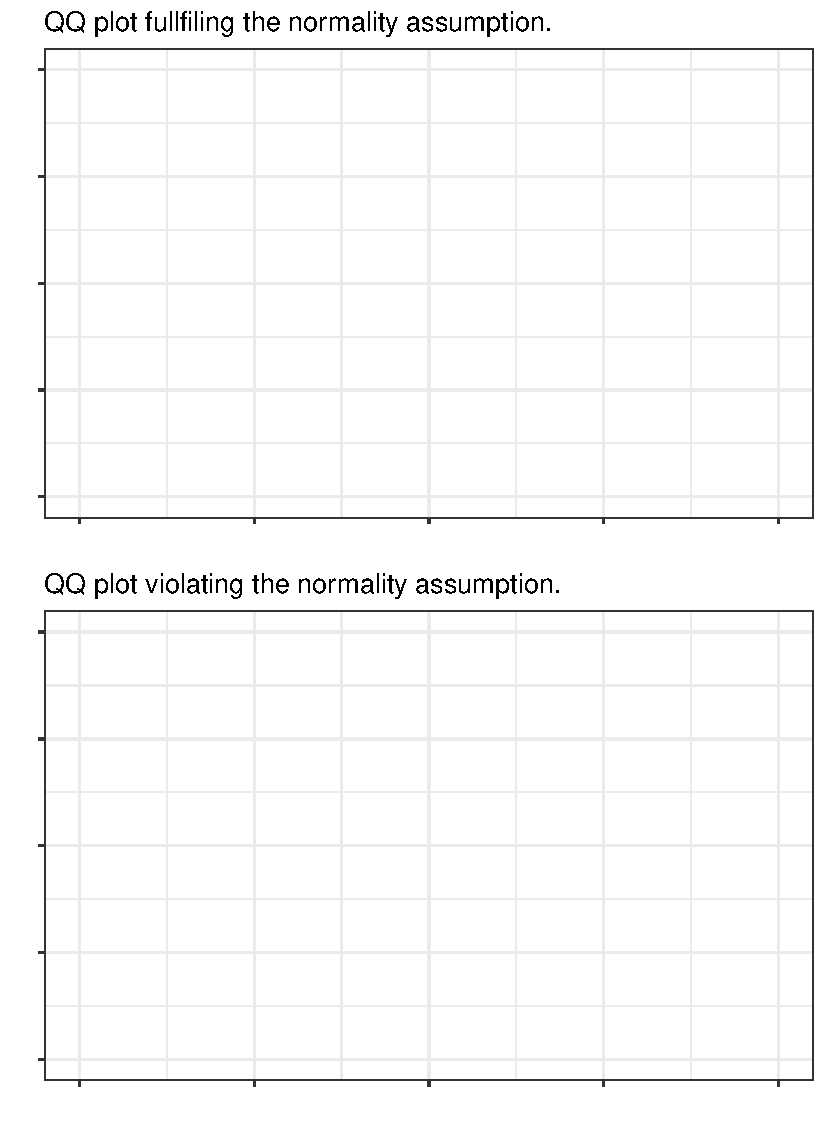
\includegraphics[width=\maxwidth]{img/regression-04-1} 

}



 
\clearpage
% -----------------------------------------------------------------------

\section{Aufgabe \hfill (10 Punkte)}

Sie rechnen eine lineare Regression um nach einem Feldexperiment den
Zusammenhang zwischen Trockengewicht kg/m$^2$ (\textit{drymatter}) und
Wassergabe l/m$^2$ (\textit{water}) bei Spargel zu bestimmen. Sie erhalten
folgende Datentabelle.

\begin{knitrout}
\definecolor{shadecolor}{rgb}{0.969, 0.969, 0.969}\color{fgcolor}\begin{table}[!h]
\centering\begingroup\fontsize{12}{14}\selectfont

\begin{tabular}{ccccc}
\toprule
.id & drymatter & water & .fitted & .resid\\
\midrule
1 & 31.3 & 13.8 & 30.3 & \\
2 & 34.5 & 17.8 & 37.3 & \\
3 & 18.2 & 8.9 & 21.7 & \\
4 & 39.3 & 17.7 & 37.3 & \\
5 & 28.3 & 12.9 & 28.8 & \\
\addlinespace
6 & 26.3 & 10.6 & 24.7 & \\
7 & 22.0 & 8.2 & 20.5 & \\
8 & 20.9 & 8.8 & 21.5 & \\
9 & 27.2 & 11.3 & 25.9 & \\
\bottomrule
\end{tabular}
\endgroup{}
\end{table}

\end{knitrout}

\begin{enumerate}
\item Erg{\"a}nzen Sie die Werte in der Spalte \texttt{.resid} in der obigen
  Tabelle. Geben Sie den Rechenweg und Formel mit an! \textbf{(4 Punkte)}
\item Zeichnen Sie den sich aus der obigen Tabelle ergebenden
  Residualplot. Beschriften Sie die Abbildung! \textbf{(4 Punkte)}
\item Gibt es auff{\"a}llige Werte anhand des Residualplots? Begr{\"u}nden Sie Ihre
  Antwort! \textbf{(2 Punkte)}
\end{enumerate}
 
\clearpage
% -----------------------------------------------------------------------

\section{Aufgabe \hfill (8 Punkte)}



In verschiedenen Fl{\"u}{\ss}en (\textit{stream}) wurde die Anzahl an
Knochenhechten (\textit{longnose}) gez{\"a}hlt. Daneben wurden noch andere
Eigenschaften der entspechenden Fl{\"u}sse gemessen. Es ergibt sich folgender
Auszug aus den Daten. 


\begin{knitrout}
\definecolor{shadecolor}{rgb}{0.969, 0.969, 0.969}\color{fgcolor}\begin{table}[!h]
\centering
\begin{tabular}{lrrrrr}
\toprule
stream & longnose & maxdepth & so4 & acerage & no3\\
\midrule
BUFFALO\_RUN & 16 & 37 & 18.87 & 12620 & 0.61\\
MORGAN\_RUN & 76 & 130 & 5.74 & 9765 & 4.38\\
NORTH\_BR & 23 & 121 & 7.36 & 3836 & 1.32\\
DORSEY\_RUN & 8 & 160 & 20.24 & 7814 & 0.44\\
\bottomrule
\end{tabular}
\end{table}

\end{knitrout}


Sie rechnen nun eine Poisson lineare Regression auf den Daten und erhalten
folgenden \Rlogo Output.

{\small
\begin{knitrout}
\definecolor{shadecolor}{rgb}{0.969, 0.969, 0.969}\color{fgcolor}\begin{kframe}
\begin{verbatim}
## 
## Call:
## glm(formula = reformulate(response = "longnose", termlabels = wanted_vec), 
##     family = quasipoisson, data = data_tbl)
## 
## Deviance Residuals: 
##     Min       1Q   Median       3Q      Max  
## -9.2130  -3.5726  -2.4167   2.1412  11.4841  
## 
## Coefficients:
##                 Estimate   Std. Error t value   Pr(>|t|)    
## (Intercept)  1.739019358  0.429434489  4.0496  0.0001823 ***
## maxdepth     0.012324209  0.003371190  3.6557  0.0006250 ***
## so4         -0.009368754  0.018216990 -0.5143  0.6093635    
## acerage      0.000047873  0.000010487  4.5651 0.00003375 ***
## no3          0.206574195  0.054026896  3.8235  0.0003722 ***
## ---
## Signif. codes:  0 '***' 0.001 '**' 0.01 '*' 0.05 '.' 0.1 ' ' 1
## 
## (Dispersion parameter for quasipoisson family taken to be 23.001355)
## 
##     Null deviance: 2104.28  on 53  degrees of freedom
## Residual deviance: 1067.13  on 49  degrees of freedom
## AIC: NA
## 
## Number of Fisher Scoring iterations: 5
\end{verbatim}
\end{kframe}
\end{knitrout}
}

\begin{enumerate}
\item Warum wurde hier eine Poisson bzw. Quasipoisson-Verteilung gew{\"a}hlt?
  Begr{\"u}nden Sie Ihre Antwort mit dem \Rlogo Output! \textbf{(2 Punkte)}
\item K{\"o}nnen Sie die \textit{Estimate} der einzelnen Einflussvariablen
  direkt interpretieren? Begr{\"u}nden Sie Ihre Antwort! \textbf{(2 Punkte)}
\item Interpretieren Sie die \textit{nicht
      signifikanten} Effekte auf die Anzahl an Knochenhechten! \textbf{(2 Punkte)}
\item Erkl{\"a}ren Sie am \Rlogo Output wie sich die \textit{t value} Spalte
  errechnet! \textbf{(2 Punkte)}
\end{enumerate}
 
\clearpage
% -----------------------------------------------------------------------

\section{Aufgabe \hfill (10 Punkte)}



Auf einer Erdbeerplantage treten unerwartet h{\"a}ufig infizierte
Erdbeerpflanzen auf. In einem Versuch sollen verschiedende Einflussfaktoren
auf den Infektionsstatus betrachtet werden. Daf{\"u}r wurde f{\"u}r jede
Erdbeerpflanze gemessen, wieviel Wasser die Pflanze erhalten hat oder ob
die Pflanze ein neuartiges Lichtregime erhalten hatte. Zus{\"a}tzlich wurde die
Anzahl an Nematoden im Boden bestimmt. Es ergibt sich folgender Auszug aus
den Daten.

\begin{knitrout}
\definecolor{shadecolor}{rgb}{0.969, 0.969, 0.969}\color{fgcolor}\begin{table}[!h]
\centering
\begin{tabular}{lrrr}
\toprule
infected & water & light & nematodes\\
\midrule
1 & 8.75 & 1 & 0\\
1 & 10.71 & 1 & 2\\
1 & 11.91 & 1 & 2\\
1 & 9.04 & 0 & 0\\
\bottomrule
\end{tabular}
\end{table}

\end{knitrout}

Sie rechnen nun eine logistische lineare Regression auf den Daten und erhalten
folgenden \Rlogo Output.

\begin{knitrout}
\definecolor{shadecolor}{rgb}{0.969, 0.969, 0.969}\color{fgcolor}\begin{kframe}
\begin{verbatim}
## # A tibble: 3 x 4
##   term        std.error statistic p.value
##   <chr>           <dbl>     <dbl>   <dbl>
## 1 (Intercept)     1.62     2.46    0.0139
## 2 water           0.153   -2.55    0.0109
## 3 nematodes       0.138   -0.0499  0.960
\end{verbatim}
\end{kframe}
\end{knitrout}


\begin{enumerate}
\item Die Spalte \textit{estimate} wurde gel{\"o}scht. Berechnen Sie die Werte
  der Spalte \textit{estimate} aus den \Rlogo Output! \textbf{(2 Punkte)}
\item Welche Einflussfaktoren sind protektiv, welche ein Risiko? Berechnen
  Sie hierf{\"u}r zun{\"a}chst das OR aus der Spalte \textit{estimate}! \textbf{(4 Punkte)}
\item Interpretieren Sie die Spalte \textit{estimate} im Bezug auf den
  Infektionsstatus der Erdbeerpflanzen! \textbf{(2 Punkte)}
\item Was ist der Unterschied zwischen einem OR und einem RR? Geben Sie ein
  numerisches Beispiel! \textbf{(2 Punkte)}
\end{enumerate}
 
\clearpage
% -----------------------------------------------------------------------

\section{Aufgabe \hfill (7 Punkte)}



Maispflanzen sollen auf die ertragssteigerende Wirkung von verschiedenen
Einflussfaktoren untersucht werden. Gemessen wurde als Outcome die
Trockenmasse in kg/m$^2$. Daf{\"u}r wurde f{\"u}r jede Maispflanze gemessen wieviel
Wasser (l/m$^2$) die Pflanze erhalten hat oder ob die Pflanze ein
neuartiges Lichtregime (0 = alt, 1 = neu) erhalten hatte. Zus{\"a}tzlich wurde
die Anzahl an Nematoden im Boden bestimmt sowie der Eisen- und
Phosphorgehalt ($\mu$g/kg) des Bodens. Es ergibt sich folgender Auszug aus
den Daten.

\begin{knitrout}
\definecolor{shadecolor}{rgb}{0.969, 0.969, 0.969}\color{fgcolor}\begin{table}[!h]
\centering
\begin{tabular}{lrrrrr}
\toprule
water & light & P & Fe & drymatter & nematodes\\
\midrule
8.92 & 0 & 8.34 & 94.05 & 71.46 & 10\\
9.09 & 0 & 10.75 & 98.68 & 68.05 & 13\\
9.61 & 0 & 9.38 & 99.46 & 68.39 & 11\\
10.45 & 0 & 10.31 & 101.84 & 69.94 & 9\\
\bottomrule
\end{tabular}
\end{table}

\end{knitrout}

Sie rechnen nun eine Gaussian lineare Regression auf den Daten und erhalten
folgenden \Rlogo Output.

{\small
\begin{knitrout}
\definecolor{shadecolor}{rgb}{0.969, 0.969, 0.969}\color{fgcolor}\begin{kframe}
\begin{verbatim}
## 
## Call:
## lm(formula = reformulate(response = "drymatter", termlabels = wanted_vec), 
##     data = data_tbl)
## 
## Residuals:
##      Min       1Q   Median       3Q      Max 
## -7.21028 -1.82350 -0.41054  2.39584  8.33807 
## 
## Coefficients:
##             Estimate Std. Error t value            Pr(>|t|)    
## (Intercept) 67.26431    2.66346 25.2544 <0.0000000000000002 ***
## water        0.31987    0.24181  1.3228              0.1887    
## light        1.03332    0.64658  1.5981              0.1130    
## nematodes   -0.10577    0.09711 -1.0892              0.2785    
## ---
## Signif. codes:  0 '***' 0.001 '**' 0.01 '*' 0.05 '.' 0.1 ' ' 1
## 
## Residual standard error: 3.1548 on 106 degrees of freedom
## Multiple R-squared:  0.058299,	Adjusted R-squared:  0.031647 
## F-statistic: 2.1874 on 3 and 106 DF,  p-value: 0.093818
\end{verbatim}
\end{kframe}
\end{knitrout}
}


\begin{enumerate}
\item Welche der Einflussfaktoren sind signifikant? Begr{\"u}nden Sie Ihre
  Antwort! \textbf{(3 Punkte)}
\item Interpretieren Sie die Spalte \textit{estimate} im Bezug auf den
  Ertrag in Trockenmasse der Maispflanzen! \textbf{(2 Punkte)}
\item Sind die Residuals approximativ Normalverteilt? Begr{\"u}nden Sie Ihre Antwort! \textbf{(2 Punkte)}
\end{enumerate}
 
\clearpage
% -----------------------------------------------------------------------

\section{Aufgabe \hfill (6 Punkte)}

Sie erhalten folgende R Ausgabe der Funktion lm().

\begin{knitrout}
\definecolor{shadecolor}{rgb}{0.969, 0.969, 0.969}\color{fgcolor}\begin{kframe}
\begin{verbatim}
## 
## Call:
## lm(formula = rsp ~ trt, data = data_tbl)
## 
## Residuals:
##      Min       1Q   Median       3Q      Max 
## -3.00000 -1.14286  0.42857  1.10714  2.00000 
## 
## Coefficients:
##             Estimate Std. Error t value         Pr(>|t|)    
## (Intercept) 16.57143    0.60609 27.3415 0.00000000009918 ***
## trtB         1.42857    0.93895  1.5215           0.1591    
## ---
## Signif. codes:  0 '***' 0.001 '**' 0.01 '*' 0.05 '.' 0.1 ' ' 1
## 
## Residual standard error: 1.6036 on 10 degrees of freedom
## Multiple R-squared:  0.18797,	Adjusted R-squared:  0.10677 
## F-statistic: 2.3148 on 1 and 10 DF,  p-value: 0.15912
\end{verbatim}
\end{kframe}
\end{knitrout}


\begin{enumerate}
\item Ist die Annahme der Normalverteilung an das Outcome \textit{rsp} erf{\"u}llt?
  Begr{\"u}nden Sie die Antwort! \textbf{(2 Punkte)}
\item Wie gro{\ss} ist der Effekt des \textit{Trt}? Liegt ein signifikanter
  Effekt vor? Geben Sie die Formel und den Rechenweg mit an! \textbf{(2 Punkte)}
\item Schreiben Sie das Ergebnis der \Rlogo Ausgabe in einen Satz nieder, der die
  Information zum Effekt und der Signifikanz enth{\"a}lt! \textbf{(2 Punkte)} 
\end{enumerate}
 
\clearpage
% -----------------------------------------------------------------------

\section{Aufgabe \hfill (11 Punkte)}

In einem Experiment zur Steigerung der Milchleistung (\textit{gain}) von
K{\"u}hen wurden zwei Arten von Musik in den St{\"a}llen gespielt. Zum einen ruhige
Musik (\textit{calm}) und eher flotte Musik (\textit{pop}). Die Messungen
wurden an jeder Kuh (\textit{subject}) wiederholt durchgef{\"u}hrt. Dar{\"u}ber
hinaus wurden verschiedene St{\"a}lle (\textit{barn}) mit der Musik bespielt.

\begin{knitrout}
\definecolor{shadecolor}{rgb}{0.969, 0.969, 0.969}\color{fgcolor}\begin{kframe}
\begin{verbatim}
## Linear mixed model fit by REML ['lmerMod']
## Formula: gain ~ attitude + (1 | subject) + (1 | barn)
##    Data: data_tbl
## 
## REML criterion at convergence: 799.4
## 
## Scaled residuals: 
##      Min       1Q   Median       3Q      Max 
## -1.97569 -0.54806 -0.10067  0.54766  3.49556 
## 
## Random effects:
##  Groups   Name        Variance Std.Dev.
##  barn     (Intercept)  233.05  15.266  
##  subject  (Intercept) 4107.89  64.093  
##  Residual              698.53  26.430  
## Number of obs: 83, groups:  barn, 7; subject, 6
## 
## Fixed effects:
##             Estimate Std. Error t value
## (Intercept) 201.7777    27.1030  7.4448
## attitudepop -18.6662     5.8072 -3.2143
## 
## Correlation of Fixed Effects:
##             (Intr)
## attitudepop -0.106
\end{verbatim}
\end{kframe}
\end{knitrout}


\begin{enumerate}
\item Ist die Annahme der Normalverteilung an das Outcome \textit{gain} erf{\"u}llt?
  Begr{\"u}nden Sie Ihre Antwort! \textbf{(2 Punkte)}
\item Wie gro{\ss} ist der Effekt der Musikart \textit{attitude}? Liegt ein signifikanter
  Effekt vor? Sch{\"a}tzen Sie den p-Wert mit einem kritischen t-Wert von $T_k
  = 1.96$ ab. Begr{\"u}nden und visualisieren Sie Ihre Antwort und
  Entscheidung! \textbf{(3 Punkte)}
\item Was ist der Unterschied zwischen einem "`random"' und "`fixed"'
  Effekt. Gehen Sie in der Begr{\"u}ndung Ihrer Antwort auf dieses konkrete
  Beispiel ein! \textbf{(3 Punkte)}
\item Wie gro{\ss} ist die Varianz, die durch die zuf{\"a}lligen Effekte erkl{\"a}rt wird? \textbf{(1 Punkt)}
\item Schreiben Sie das Ergebnis der \Rlogo Ausgabe in einen Satz nieder, der die
  Information zum Effekt und der Signifikanz enth{\"a}lt! \textbf{(2 Punkte)}
\end{enumerate}
 
\clearpage
% -----------------------------------------------------------------------

\section{Aufgabe \hfill (9 Punkte)}

Nach einem Pilotversuch k{\"o}nnen Sie f{\"u}r vier D{\"u}ngestufen die jeweiligen
Ertr{\"a}ge ermitteln. F{\"u}r den Hauptversuch wollen Sie nun die ben{\"o}tigte
Fallzahl absch{\"a}tzen. 



\begin{enumerate}
\item Skizzieren Sie den zugeh{\"o}rigen Boxplot f{\"u}r die vier D{\"u}ngestufen mit
  folgenden Informationen.
\begin{knitrout}
\definecolor{shadecolor}{rgb}{0.969, 0.969, 0.969}\color{fgcolor}\begin{table}[!h]
\centering
\begin{tabular}{cccccccc}
\toprule
treatment & mean & median & min & max & quartile\_1st & quartile\_3rd & var\\
\midrule
A & 12.67 & 13 & 7 & 16 & 11.75 & 14.25 & 5.70\\
B & 19.83 & 19 & 17 & 24 & 18.75 & 21.00 & 4.33\\
C & 14.75 & 15 & 4 & 20 & 13.50 & 17.00 & 17.48\\
D & 17.08 & 15 & 13 & 25 & 14.00 & 19.00 & 16.99\\
\bottomrule
\end{tabular}
\end{table}

\end{knitrout}
Beschriften Sie die Achsen entsprechend! \textbf{(4 Punkte)}
\item Berechnen Sie die ben{\"o}tigten Fallzahlen f{\"u}r die Gruppenvergleiche mit
\begin{equation*}
  n_{Gruppe} = \cfrac{2 \cdot (1.96 + 0.77)^2}{\left(\cfrac{\Delta}{s_{pool}}\right)^2}
\end{equation*}
Nutzen Sie hierf{\"u}r das gepoolte $s_{pool}$ mit $s_{pool} = (s_1 + s_2)/2$! \textbf{(4 Punkte)}
\item Was ist die Fallzahl, die Sie f{\"u}r den Versuch ben{\"o}tigen? \textbf{(1 Punkte)}
\end{enumerate} 
\clearpage
% -----------------------------------------------------------------------

\section{Aufgabe \hfill (10 Punkte)}

In einem Feldexperiment f{\"u}r die Bodendurchl{\"a}ssigkeit wurde der Niederschlag
pro Parzelle sowie der durchschnittliche Ertrag gemessen. Es ergibt sich
folgende Datentabelle. 

\begin{table}[!h]
\centering
\begin{tabular}{cc}
\toprule
water & drymatter\\
\midrule
20 & 12\\
21 & 17\\
24 & 13\\
21 & 19\\
17 & 15\\
\bottomrule
\end{tabular}
\end{table}



\begin{enumerate}
\item Erstellen Sie den Scatter-Plot f{\"u}r die Datentabelle. Beschriften Sie
  die Achsen entsprechend! \textbf{(4 Punkte)}
\item Zeichnen Sie eine Gerade durch die Punkte! \textbf{(1 Punkt)}
\item Beschriften Sie die Gerade mit den g{\"a}ngigen statistischen Ma{\ss}zahlen! \textbf{(3 Punkte)}
\item Wenn kein Effekt von dem Niederschlag auf das Trockengewicht
  vorhanden w{\"a}re, wie w{\"u}rde die Gerade verlaufen und welche Werte w{\"u}rden die
  statistischen Ma{\ss}zahlen annehmen? \textbf{(2 Punkt)}
\end{enumerate} 
\clearpage
% -----------------------------------------------------------------------

\section{Aufgabe \hfill (7 Punkte)}

In einer Studie zur "`Arbeitssicherheit auf dem Feld"' wurde gemessen wie viele
Stunden auf einem Feld gefahren wurden und wie oft der Fahrer dabei drohte
einzunicken. Es ergab sich folgende Abbildung. 



{\centering 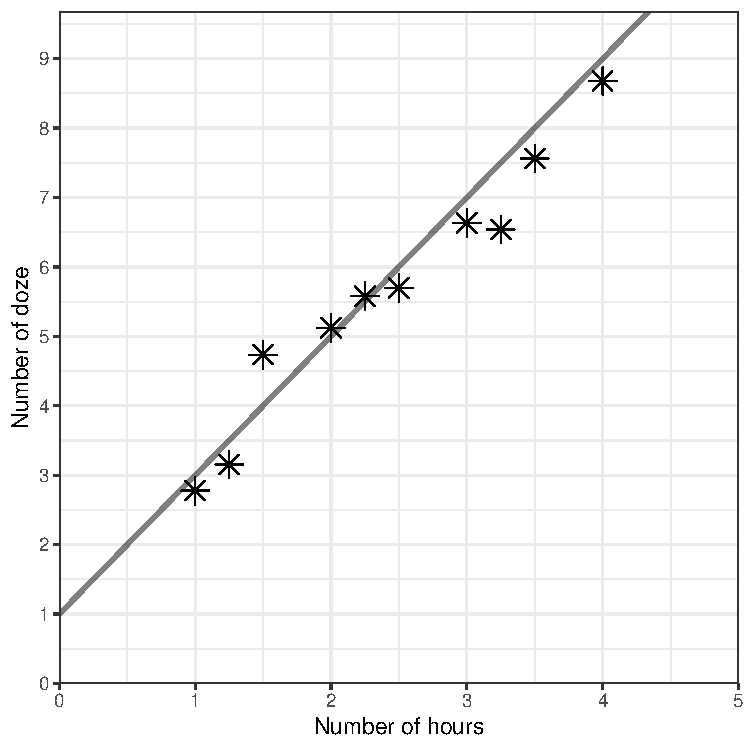
\includegraphics[width=\maxwidth]{img/scatter-02-1} 

}




\begin{enumerate}
\item Erstellen Sie die Regressionsgleichung aus der obigen Abbildung in
  der Form $y \sim \beta_0 + \beta_1 \cdot x$! \textbf{(2 Punkte)}
\item Beschriften Sie die Gerade mit den Parametern der linearen
  Regressionsgleichung! \textbf{(2 Punkte)}
\item Liegt ein Zusammenhang zwischen der Anzahl an gefahrenen Runden und
  der M{\"u}digkeit vor? Begr{\"u}nden Sie Ihre Antwort! \textbf{(2 Punkte)}
\item Wenn kein Zusammenhang zu beobachten w{\"a}re, wie w{\"u}rde die Gerade aussehen? \textbf{(1 Punkt)}
\end{enumerate} 
\clearpage
% -----------------------------------------------------------------------

\section{Aufgabe \hfill (6 Punkte)}

\begin{enumerate}
\item Erkl{\"a}ren Sie den Zusammenhang zwischen Stichprobe und Grundgesamtheit
  an einem Schaubild! \textbf{(3 Punkte)}
\item Was ist der Unterschied zwischen $\mu$ und $\sigma$ und $\bar{x}$ und
  $s$ im Kontext der Stichprobe und Grundgesamtheit? \textbf{(2 Punkte)}
\item Warum m{\"u}ssen wir {\"u}berhaupt zwischen einer Stichprobe und einer
  Grundgesamtheit unterscheiden? \textbf{(1 Punkt)}
\end{enumerate} 
\clearpage
% -----------------------------------------------------------------------

\section{Aufgabe \hfill (6 Punkte)}



Geben ist folgende 2x2 Kreuztabelle. 

\begin{center}
  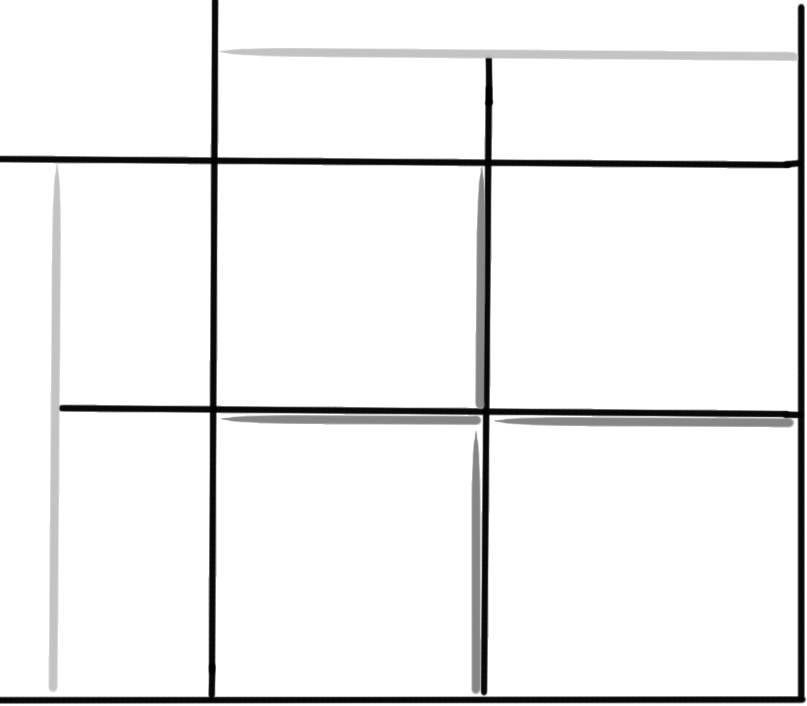
\includegraphics[width = 14cm]{/Users/kruppajo/Documents/GitHub/exam/question/img/text-error-cross-table}
\end{center}

\begin{enumerate}
\item Tragen Sie folgende Fachbegriffe korrekt in die 2x2 Kreuztabelle ein! \textbf{(6 Punkte)}
  \begin{itemize}
  \item (Unbekannte) Wahrheit	
  \item H$_0$ wahr
  \item H$_0$ falsch
  \item H$_0$ abgelehnt
  \item H$_0$ beibehalten
  \item Testentscheidung
  \item $\alpha$-Fehler
  \item $\beta$-Fehler
  \item Richtige Entscheidung
  \item 5\%
  \item 20\%
  \end{itemize}
\end{enumerate}



 
\clearpage
% -----------------------------------------------------------------------

\section{Aufgabe \hfill (4 Punkte)}



Im folgenden ist eine t-Verteilung abgebildet. Erg{\"a}nzen Sie die Abbidlung wie folgt.

\begin{enumerate}
\item Zeichnen Sie das Signifikanzniveau $\alpha$ in die Abbildung! \textbf{(1 Punkte)} 
\item Zeichnen Sie einen nicht signifikant p-Wert in die Abbildung! \textbf{(1 Punkt)} 
\item Erg{\"a}nzen Sie "`$\bar{y}_1 = \bar{y}_2$"'! \textbf{(1 Punkt)} 
\item Erg{\"a}nzen Sie "`$A = 0.95$"'! \textbf{(1 Punkt)} 
\end{enumerate}



{\centering 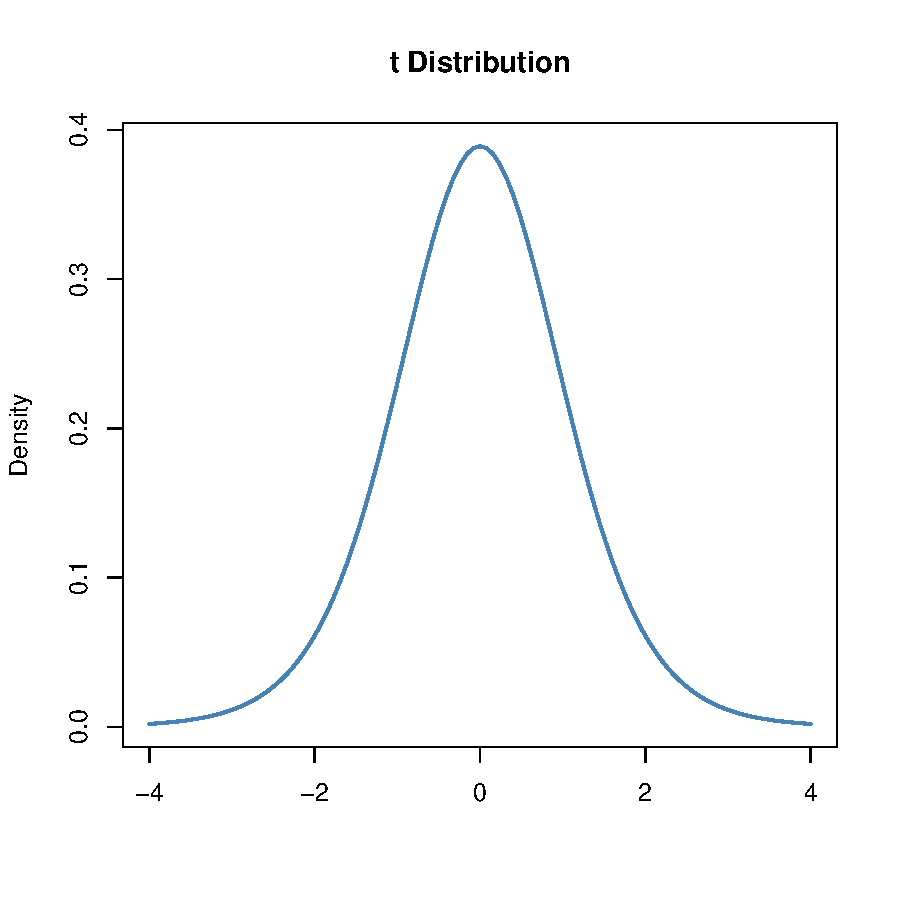
\includegraphics[width=\maxwidth]{img/statistisches-testen-3-1} 

}


 
\clearpage
% -----------------------------------------------------------------------

\section{Aufgabe \hfill (8 Punkte)}



Sie rechnen einen t-Test. Sie sch{\"a}tzen einen Mittelwertsunterschied. 

\begin{enumerate}
\item Beschriften Sie die untenstehende Abbildung mit der
  Signifikanzschwelle! \textbf{(1 Punkt)}
\item Erg{\"a}nzen Sie eine Relevanzschwelle! \textbf{(1 Punkt)} 
\item Skizieren Sie in die
  untenstehende Abbildung f{\"u}nf einzelne Konfidenzintervalle (a-e) mit den
  jeweiligen Eigenschaften! \textbf{(6 Punkte)}
  \begin{itemize}
  \item[(a)] Ein signifikantes, nicht relevantes Konfidenzintervall 	
  \item[(b)] Ein Konfidenzintervall mit h{"o}hererVarianz $s_p$ in der Stichprobe als der Rest der Konfidenzintervalle 	
  \item[(c)] Ein nicht signifikantes, relevantes Konfidenzintervall 	
  \item[(d)] Ein Konfidenzintervall mit niedriger Varianz $s_p$ in der Stichprobe als der Rest der Konfidenzintervalle 
  \item[(e)] Ein signifikantes, relevantes Konfidenzintervall
  \end{itemize}
\end{enumerate}

\begin{center}
  
\includegraphics[height = 8cm]{/Users/kruppajo/Documents/GitHub/exam/question/img/statistisches-testen-04}
\end{center}


 
\clearpage
% -----------------------------------------------------------------------

\section{Aufgabe \hfill (6 Punkte)}

Gegeben ist die vereinfachte Formel f{\"u}r den Zweistichproben t-Test mit der
gepoolten Standardabweichung $s_p$ und gleicher Gruppengr{\"o}sse $n_g$ der
beiden Sample.

\begin{equation*}
  \label{eq:1}
  T = \cfrac{\bar{y}_1 - \bar{y}_2}{s_p \cdot \sqrt{\tfrac{2}{n_g}}}
\end{equation*}

Welche Auswirkung hat die {\"A}nderungen der jeweiligen statistischen Masszahl
auf den T-Wert und damit auf die \textit{vermutliche} Signifikanz? F{\"u}llen
Sie hierzu die untenstehende Tabelle aus! \textbf{(6 Punkte)}

\begin{center}
  \large
  \begin{tabular}[c]{l|l|l|l|l|l|l|l}
    & T Statistik & $Pr(D|H_0)$ & $KI_{1-\alpha}$ & & T Statistik & $Pr(D|H_0)$ & $KI_{1-\alpha}$\strut\\ 
    \hline
    \textbf{$\Delta\; \uparrow$} & \hspace{2cm} & \hspace{2cm}  & \hspace{2cm} & \textbf{
                                                          $\Delta\; \downarrow$} &
                                                                          \hspace{2cm} & \hspace{2cm}  & \hspace{2cm}\strut\\
    \hline
        \textbf{$s\; \uparrow$} & \hspace{2cm} & \hspace{2cm}  & \hspace{2cm} & \textbf{
                                                          $s\; \downarrow$} &
                                                                          \hspace{2cm}
                                                & \hspace{2cm}  & \hspace{2cm}\strut\\
    \hline
        \textbf{$n\; \uparrow$} & \hspace{2cm} & \hspace{2cm}  & \hspace{2cm} & \textbf{
                                                          $n\; \downarrow$} &
                                                                          \hspace{2cm}
                                                & \hspace{2cm}  & \hspace{2cm}\strut\\
    \hline
  \end{tabular}
\end{center}
 
\clearpage
% -----------------------------------------------------------------------

\section{Aufgabe \hfill (8 Punkte)}



Sie haben folgende Aussage gegeben.

\begin{center}
  \Large\textbf{Bin ich im Fr{"u}hling?}
\end{center}

\begin{enumerate}
\item Erkl{\"a}ren Sie den Gedankengang der Testtheorie sowie des Falsifikationsprinzips an der Aussage! \textbf{(4 Punkte)}
\item Erkl{\"a}ren Sie Ihre Entscheidung zu der Aussage! \textbf{(3 Punkte)}
\item Sch{\"a}tzen Sie den p-Wert zu der Aussage ab! \textbf{(1 Punkt)}
\end{enumerate}

 
\clearpage
% -----------------------------------------------------------------------

\section{Aufgabe \hfill (8 Punkte)}



\begin{quote}
  >>Ohne ausreichende Zufuhr von Vitamin C stellen sich nach 68 Tagen die
  ersten Symptome ein; die ersten Toten sind nach 98 Tagen zu beklagen;
  nach 123 Tagen rafft die Skorbut eine ganze Schiffsbesatzung dahin.<<
\end{quote}


\begin{enumerate}
\item Stellen Sie den Verlauf der Skorbuterkrankung auf einem Schiff mit
  einer typischen Anzahl an Matrosen dar. Welche Annahmen haben
  Sie getroffen? Beschriften Sie die Achsen entsprechend!
  \textbf{(4 Punkte)}
\item Schiffarzt James Lind (1716-1794) ist dem Ph{\"a}nomen Skorbut
  systematisch nachgegangen. Wie w{\"u}rden Sie solch ein Experiment planen und
  welche (ethischen) Probleme sehen Sie? \textbf{(4 Punkte)}
\end{enumerate} 
\clearpage
% -----------------------------------------------------------------------

\section{Aufgabe \hfill (11 Punkte)}

Der Wissenschaftler Pettenkofer arbeitete streng naturwissenschaftlich-experimentell und gilt
als Begr{\"u}nder der experimentellen Hygiene (``Konditionalhygiene''). Auch
seine Untersuchungen zu Kleidung, Heizung, L{\"u}ftung, Kanalisation und
Wasserversorgung trugen experimentelle Z{\"u}ge. Pettenkofer war ein Positivist, das hei{\ss}t, er erkannte ausschlie{\ss}lich
sichtbare, zum Beispiel in Experimenten gewonnene Tatsachen als
Erkenntnisquelle an.

\begin{shaded}
  Pettenkofer unterlief ein Irrtum, der bis heute
  nachwirkt, indem viele Menschen glauben, es gebe eine ``Atmende Wand'':
  Er stellte bei fr{\"u}hen Luftwechsel-Messungen in einem Zimmer fest, dass
  sich nach dem vermeintlichen Abdichten s{\"a}mtlicher Fugen die
  Luftwechselrate weniger als erwartet verminderte. Daraus schlussfolgerte
  er einen erheblichen Luftaustausch durch die Ziegelw{\"a}nde
  hindurch. Vermutlich kam er nicht darauf, den Kamin eines im Raum
  befindlichen Ofens abzudichten. Luftaustausch durch die Zimmerw{\"a}nde
  hindurch sei, so Pettenkofer, ein wesentlicher Beitrag zur Reinigung der
  Raumluft.
\end{shaded}

\begin{enumerate}
\item Bestimmen Sie das $y$ bzw. den Endpunkt/Outcome f{\"u}r das Experiment ``Atmende Wand''. Wie
  messen Sie den Endpunkt? \textbf{(1 Punkt)}
\item Bestimmen Sie m{\"o}gliche Einflussfaktoren auf den Endpunkt! Begründen Sie Ihre Entscheidung! \textbf{(2 Punkt)}
\item Beschreiben Sie das Modell in der Form $y \sim x$! \textbf{(1 Punkt)}
\item Wie realisieren Sie Wiederholung in
  dem Experiment? Skizieren Sie das Experiment! \textbf{(2 Punkte)}
\item Wie k{\"o}nnten Sie das Experiment graphisch darstellen? Was befindet
  sich auf der x-Achse und was auf der y-Achse? Beschriften Sie die Achsen entsprechend!
  \textbf{(2 Punkte)}
\item Basiert die heutige Wissenschaft auch auf dem Positivismus? Begründen Sie Ihre Antwort! \textbf{(2 Punkte)}
\end{enumerate}
 
\clearpage
% -----------------------------------------------------------------------

\section{Aufgabe \hfill (12 Punkte)}

Nach einem Experiment mit zwei Pestiziden (\textit{RoundUp} und
\textit{GoneEx}) ergibt sich die folgende Datentabelle mit dem gemessenen
Trockengewicht (\textit{drymatter}) von Weizen.

\begin{table}[!h]
\centering
\begin{tabular}{cc}
\toprule
pesticide & drymatter\\
\midrule
RoundUp & 17\\
RoundUp & 15\\
RoundUp & 18\\
GoneEx & 15\\
GoneEx & 16\\
\addlinespace
RoundUp & 14\\
GoneEx & 14\\
GoneEx & 15\\
RoundUp & 18\\
GoneEx & 16\\
\addlinespace
GoneEx & 16\\
RoundUp & 16\\
RoundUp & 18\\
\bottomrule
\end{tabular}
\end{table}



\begin{enumerate}
  \item Formulieren Sie die wissenschaftliche Fragestellung! \textbf{(1 Punkt)}
  \item Formulieren Sie das statistische Hypothesenpaar! \textbf{(2
      Punkte)}
  \item Bestimmen Sie die Teststatistik $T_{calc}$ eines Student t-Tests f{\"u}r den
  Vergleich der beiden Pestizide. Geben Sie den Rechenweg und die Formeln
  mit an! \textbf{(5 Punkte)}
\item Treffen Sie mit $T_{\alpha = 5\%} = 2.04$ und dem berechneten $T_{calc}$ eine Aussage
  zur Nullhypothese! \textbf{(2 Punkte)}
\item Wenn Sie keinen Unterschied zwischen den beiden Pestiziden erwarten
  w{\"u}rden, wie gro{\ss}e w{\"a}re dann die Teststatistik $T_{calc}$? Begr{\"u}nden Sie Ihre
  Antwort! \textbf{(2 Punkte)}
\end{enumerate} 
\clearpage
% -----------------------------------------------------------------------

\section{Aufgabe \hfill (13 Punkte)}

Das Gewicht von K{\"u}ken wurde \textit{vor} der Behandlung mit STARTex und 1
Woche \textit{nach} der Behandlung gemessen. Es ergibt sich die folgende
Datentabelle.

\begin{table}[!h]
\centering
\begin{tabular}{ccc}
\toprule
animal\_id & before & after\\
\midrule
1 & 14 & 18\\
2 & 9 & 16\\
3 & 17 & 16\\
4 & 13 & 16\\
5 & 20 & 15\\
\addlinespace
6 & 15 & 14\\
7 & 10 & 16\\
\bottomrule
\end{tabular}
\end{table}



\begin{enumerate}
\item Formulieren Sie die Fragestellung! \textbf{(1 Punkt)}
\item Formulieren Sie das statistische Hypothesenpaar! \textbf{(2
    Punkte)}
\item Bestimmen Sie die Teststatistik $T_{calc}$ eines gepaarten t-Tests f{\"u}r den
  Vergleich der beiden Zeitpunkte. Geben Sie den Rechenweg und die Formeln
  mit an! \textbf{(4 Punkte)}
\item Treffen Sie mit $T_{\alpha = 5\%} = 2.04$ und dem berechneten $T_{calc}$ eine Aussage
  zur Nullhypothese! \textbf{(2 Punkte)}
\item Wenn Sie keinen Unterschied zwischen den beiden Zeitpunkten erwarten
  w{\"u}rden, wie gro{\ss}e w{\"a}re dann die Teststatistik $T_{calc}$? Begr{\"u}nden Sie Ihre
  Antwort! \textbf{(2 Punkte)}
\item Sch{\"a}tzen Sie $Pr(D|H_0)$ ab. Begr{\"u}nden Sie Ihre Antwort! \textbf{(2
    Punkte)}
\end{enumerate} 
\clearpage
% -----------------------------------------------------------------------

\section{Aufgabe \hfill (10 Punkte)}

Sie erhalten folgende \Rlogo Ausgabe der Funktion \texttt{t.test()}.

\begin{knitrout}
\definecolor{shadecolor}{rgb}{0.969, 0.969, 0.969}\color{fgcolor}\begin{kframe}
\begin{verbatim}
## 
## 	Two Sample t-test
## 
## data:  drymatter by Fe
## t = 3.0302, df = 10, p-value = 0.012673
## alternative hypothesis: true difference in means between group high and group low is not equal to 0
## 95 percent confidence interval:
##  1.4973874 9.8168983
## sample estimates:
## mean in group ctrl mean in group trt2 
##          18.800000          13.142857
\end{verbatim}
\end{kframe}
\end{knitrout}


\begin{enumerate}
  \item Formulieren Sie das statistische Hypothesenpaar! \textbf{(2
Punkte)}
\item Liegt ein signifikanter Unterschied zwischen den Gruppen vor?
  Begr{\"u}nden Sie Ihre Antwort! \textbf{(2 Punkte)}
\item Skizieren Sie eine Abbildung in der Sie $T_{calc}$, $Pr(D|H_0)$, $A=0.95$,
  sowie $T_{\alpha=5\%} = |2.23|$ einzeichnen! \textbf{(4 Punkte)}
\item Beschriften Sie die Abbildung entsprechend! \textbf{(2 Punkte)}  
\end{enumerate} 
\clearpage
% -----------------------------------------------------------------------

\section{Aufgabe \hfill (8 Punkte)}

Sie erhalten folgende \Rlogo Ausgabe der Funktion \texttt{t.test()}.

\begin{knitrout}
\definecolor{shadecolor}{rgb}{0.969, 0.969, 0.969}\color{fgcolor}\begin{kframe}
\begin{verbatim}
## 
## 	Two Sample t-test
## 
## data:  freshmatter by N
## t = -1.33069, df = 12, p-value = 0.20802
## alternative hypothesis: true difference in means between group high and group low is not equal to 0
## 95 percent confidence interval:
##  -4.1444191  1.0015620
## sample estimates:
## mean in group mid mean in group low 
##         13.857143         15.428571
\end{verbatim}
\end{kframe}
\end{knitrout}


\begin{enumerate}
  \item Formulieren Sie die wissenschaftliche Fragestellung! \textbf{(2
Punkte)}
\item Liegt ein signifikanter Unterschied zwischen den Gruppen vor?
  Begr{\"u}nden Sie Ihre Antwort! \textbf{(2 Punkte)}
\item Skizieren Sie das sich ergebende 95\% Konifidenzintervall! \textbf{(2 Punkte)}
\item Beschriften Sie die Abbildung und
  das 95\% Konfidenzintervall entsprechend! \textbf{(2 Punkte)}  
\end{enumerate} 
\clearpage
% -----------------------------------------------------------------------

\section{Aufgabe \hfill (8 Punkte)}

Sie erhalten folgende \Rlogo Ausgabe der Funktion \texttt{t.test()}.

\begin{knitrout}
\definecolor{shadecolor}{rgb}{0.969, 0.969, 0.969}\color{fgcolor}\begin{kframe}
\begin{verbatim}
## 
## 	Two Sample t-test
## 
## data:  drymatter by Fe
## t = -5.04207, df = 10, p-value = 0.00050509
## alternative hypothesis: true difference in means between group high and group low is not equal to 0
## 95 percent confidence interval:
##  -12.1944350  -4.7198507
## sample estimates:
## mean in group high  mean in group low 
##          13.400000          21.857143
\end{verbatim}
\end{kframe}
\end{knitrout}


\begin{enumerate}
  \item Formulieren Sie das statistische Hypothesenpaar! \textbf{(2
Punkte)}
\item Liegt ein signifikanter Unterschied zwischen den Gruppen vor?
  Begr{\"u}nden Sie Ihre Antwort! \textbf{(2 Punkte)}
\item Skizieren Sie die sich ergebenden Boxplots! Welche Annahmen an die Daten haben Sie getroffen? Begr{\"u}nden Sie Ihre Antwort! \textbf{(4 Punkte)} 
\end{enumerate}
 
\clearpage
% -----------------------------------------------------------------------

\section{Aufgabe \hfill (8 Punkte)}

Sie erhalten folgende \Rlogo Ausgabe der Funktion \texttt{t.test()}.

\begin{knitrout}
\definecolor{shadecolor}{rgb}{0.969, 0.969, 0.969}\color{fgcolor}\begin{kframe}
\begin{verbatim}
## 
## 	Paired t-test
## 
## data:  drymatter by Fe
## t = 0, df = 8, p-value = 1
## alternative hypothesis: true mean difference is not equal to 0
## 95 percent confidence interval:
##  -1.9597267  1.9597267
## sample estimates:
## mean difference 
##               0
\end{verbatim}
\end{kframe}
\end{knitrout}


\begin{enumerate}
  \item Formulieren Sie das statistische Hypothesenpaar! \textbf{(2
Punkte)}
\item Liegt ein signifikanter Unterschied zwischen den Gruppen vor?
  Begr{\"u}nden Sie Ihre Antwort! \textbf{(2 Punkte)}
\item Skizzieren Sie den sich ergebenden Datensatz mit $n = 4$! Beobachtungen! \textbf{(2 Punkte)} 
\item Skizieren Sie die sich ergebenden Boxplots! Welche Annahmen an die Daten haben Sie getroffen? Begr{\"u}nden Sie Ihre Antwort! \textbf{(2 Punkte)} 
\end{enumerate}
 
\clearpage
% ----------------------------------------------------------------------- 

\section{Aufgabe \hfill (12 Punkte)}

Die Anzahl an Nematoden wurde vor und nach einer Behandlung mit einem
bioaktiven D{\"u}nger gez{\"a}hlt. Es ergibt sich folgende Datentabelle.

\begin{table}[!h]
\centering
\begin{tabular}{ccccccc}
\toprule
Vorher & Nachher & Differenz & Vorzeichen & Rang & Positiv Rang & Negativ Rang\\
\midrule
9 & 12 &  &  &  &  & \\
7 & 12 &  &  &  &  & \\
11 & 13 &  &  &  &  & \\
10 & 12 &  &  &  &  & \\
8 & 14 &  &  &  &  & \\
\addlinespace
8 & 12 &  &  &  &  & \\
10 & 12 &  &  &  &  & \\
6 & 12 &  &  &  &  & \\
14 & 9 &  &  &  &  & \\
13 & 13 &  &  &  &  & \\
\addlinespace
11 & 11 &  &  &  &  & \\
6 & 12 &  &  &  &  & \\
9 & 13 &  &  &  &  & \\
10 & 10 &  &  &  &  & \\
11 & 11 &  &  &  &  & \\
\bottomrule
\end{tabular}
\end{table}



\begin{enumerate}
\item Erg{\"a}nzen Sie die obige Tabelle mit den notwendigen Informationen, die
  Sie ben{\"o}tigen um einen Wilcoxon-Vorzeichen-Rang-Test zu rechnen!
  \textbf{(4 Punkte)}
\item Bestimmen Sie die Teststatistik $W$ mit $W = \min(T_{-}; T_{+})$ und
  berechnen Sie den erwarteten Wert $\mu_W = \cfrac{n \cdot (n + 1)}{4}$!
  \textbf{(2 Punkte)}
\item Berechnen Sie anschlie{\ss}end den $z$-Wert mit $z = \cfrac{W -
    \mu_W}{0}$! \textbf{(2 Punkte)}
\item Liegt mit einer Signifikanzschwelle von $z =
  1.96$ ein Unterschied zwischen den beiden Zeitpunkten vor? Begr{\"u}nden Sie
  Ihre Antwort! \textbf{(2 Punkte)} 
\item Berechnen Sie die Effektst{\"a}rke mit $r = |\frac{z}{\sqrt{n}}| $ und
  interpretieren Sie die Effektst{\"a}rke! \textbf{(2 Punkte)} 
\end{enumerate} 
\clearpage
% -----------------------------------------------------------------------  

\section{Aufgabe \hfill (8 Punkte)}



Nach einer Behandlung mit RootsGoneX wurde die mittelere Anzahl an Wurzeln
an der invasiven Lupine (\textit{Lupinus polyphyllus}) gez{\"a}hlt. Es ergab sich
folgender Datensatz an mittleren Wurzelanzahl.

\begin{knitrout}
\definecolor{shadecolor}{rgb}{0.969, 0.969, 0.969}\color{fgcolor}\begin{table}[!h]
\centering
\begin{tabular}{cc}
\toprule
Treatment & Count\\
\midrule
RootsGoneX & 8.3\\
RootsGoneX & 10.9\\
RootsGoneX & 12.4\\
RootsGoneX & 8.0\\
RootsGoneX & 9.8\\
\addlinespace
RootsGoneX & 9.0\\
RootsGoneX & 8.0\\
Kontrolle & 20.1\\
Kontrolle & 13.6\\
Kontrolle & 9.0\\
\addlinespace
Kontrolle & 12.0\\
Kontrolle & 10.5\\
Kontrolle & 14.2\\
Kontrolle & 10.6\\
\bottomrule
\end{tabular}
\end{table}

\end{knitrout}

Rechnen Sie einen Mann-Whitney-U-Test auf den obigen Daten.

\begin{enumerate}
\item Bestimmen Sie hierf{\"u}r $U_c$ mit $U_c = n_1n_2 +
  \cfrac{n_1(n_1+1)}{2}-R_1$! \textbf{(4 Punkte)} 
\item Geben Sie eine Aussage {\"u}ber die Signifikanz von $U_c$ durch $z =
  \cfrac{U_c - \cfrac{n_1n_2}{2}}{\sqrt{\cfrac{n_1n_2(n_1+n_2+1)}{12}}}$ und
  dem kritischen Wert von $z = 1.96$. Begr{\"u}nden Sie Ihre Antwort! \textbf{(2 Punkte)} 
\item Berechnen Sie die Effektst{\"a}rke mit $r = |\frac{z}{\sqrt{n}}| $ und
  interpretieren Sie die Effektst{\"a}rke! \textbf{(2 Punkte)} 
\end{enumerate} 
\clearpage
% ----------------------------------------------------------------------- 

\section{Aufgabe \hfill (9 Punkte)}



Die Anzahl an Bl{\"u}ten der Vanilleplanze pro Box wurde nach der Gabe von
zus{\"a}tzlichen Phosporl{\"o}sung (Kontrolle, Dosis 20 und Dosis 40) bestimmt. Es
ergeben sich folgende nach der Anzahl der Bl{\"u}ten geordnete Daten.

\begin{knitrout}
\definecolor{shadecolor}{rgb}{0.969, 0.969, 0.969}\color{fgcolor}\begin{table}[!h]
\centering
\begin{tabular}{ccccc}
\toprule
Treatment & Count & Rang Kontrolle & Rang Dosis 20 & Rang Dosis 40\\
\midrule
Kontrolle & 5.0 &  &  & \\
Dosis 20 & 5.7 &  &  & \\
Kontrolle & 7.8 &  &  & \\
Kontrolle & 7.8 &  &  & \\
Kontrolle & 8.8 &  &  & \\
\addlinespace
Dosis 20 & 9.7 &  &  & \\
Dosis 40 & 9.7 &  &  & \\
Kontrolle & 10.0 &  &  & \\
Dosis 40 & 10.2 &  &  & \\
Dosis 20 & 11.3 &  &  & \\
\addlinespace
Kontrolle & 11.4 &  &  & \\
Dosis 20 & 11.7 &  &  & \\
Dosis 40 & 12.2 &  &  & \\
Dosis 20 & 12.5 &  &  & \\
Dosis 20 & 13.5 &  &  & \\
\addlinespace
Dosis 40 & 14.0 &  &  & \\
Kontrolle & 16.5 &  &  & \\
Dosis 40 & 17.3 &  &  & \\
\bottomrule
\end{tabular}
\end{table}

\end{knitrout}

Rechnen Sie einen Kruskal-Wallis-Test auf den obigen Daten.

\begin{enumerate}
\item Bestimmen Sie hierf{\"u}r $H_c$ mit $H_c =
  \cfrac{12}{n(n+1)}\left(\cfrac{R_1^2}{n_1}+\cfrac{R_2^2}{n_2}
    + \cfrac{R_3^2}{n_3}\right)
  - 3(n+1)$! \textbf{(6 Punkte)} 
\item Geben Sie eine Aussage {\"u}ber die Signifikanz von $H_c$ durch
  den kritischen Wert von $H = 5.99$! \textbf{(1 Punkt)}
\item Wie lautet die Nullhypothese die Sie mit dem Kruskal-Wallis-Test
  {\"u}berpr{\"u}fen? \textbf{(1 Punkt)}
\item Was sagt ein signifikantes Ergebnis des Kruskal-Wallis-Test in Bezug
  auf die einzelnen Gruppenvergleiche aus? \textbf{(1 Punkt)}
\end{enumerate} 
\clearpage
% ----------------------------------------------------------------------- 
\end{document}
% -----------------------------------------------------------------------
